%!TEX root = these.tex

\chapter[Taxinomie des environnements de sélection]{Taxinomie des environnements de sélection}
\minitoc
\label{chap3}
\cleardoublepage

\section{Introduction}
	Au cours du premier chapitre de ce manuscrit, nous avons identifié un certain nombre de besoins associés à des applications précises. Nous nous sommes également attachés à caractériser la nature des cibles mobiles que l'on rencontre dans ces applications, afin de permettre au lecteur d'apprécier d'une part l'ensemble des difficultés inhérentes aux tâches de sélection dans ces applications, et d'autre part la nécessité d'une assistance à la sélection.
	
	Si nous avons jusqu'ici énuméré et caractérisé ces types de cibles, avec une attention toute particulière à leur contexte applicatif, nous n'avons pas procédé à une classification systématique des cibles selon la nature de leur mouvement, définie selon des critères objectifs et des mesures quantitatives. Or, il nous apparaît que pour réellement comprendre les enjeux et défis liés à la sélection de cibles mobiles, une telle classification est nécessaire.
	
	L'objectif de ce chapitre est donc d'établir une taxinomie des cibles mobiles selon des critères objectifs et, dans la mesure du possible, permettant une quantification des valeurs auxquelles ils se rapportent. Nous commencerons par exposer nos réflexions sur les critères à retenir pour établir cette taxinomie, puis nous confronterons les cibles et leurs environnements à ces critères. Nous présenterons ensuite un modèle que nous avons développé pour décrire et générer du mouvement pseudo-aléatoire, régi par des paramètres finement contrôlés. Nous nous appuierons sur ce modèle pour compléter notre taxinomie par des mesures quantitatives et objectives.
	
	
	\section{Critères de discrimination et nature du mouvement}
	Bien qu'une \og simple \fg{} taxinomie des cibles mobiles en fonction de la nature de leur mouvement ait beaucoup d'intérêt, elle ne saurait fournir suffisamment d'informations pour guider la conception de techniques de sélection sans tenir compte de l'\emph{environnement} de sélection. En effet, la cible la plus petite, la plus rapide et la plus imprévisible imaginable est triviale à sélectionner s'il s'agit du seul objet d'intérêt dans l'environnement : il n'y a qu'une sélection possible, donc la technique de sélection optimale --- ou du moins suffisante --- consiste à permettre la sélection de la cible par la simple pression d'un bouton, ou activation d'un quelconque périphérique de saisie.
	
	En effet, du point de vue de la théorie de l'information de Shannon~\cite{shannon2001mathematical}, un seul bit d'information est à transmettre de l'utilisateur au système, correspondant à la réponse à la question suivante : \og la cible doit-elle être sélectionnée ? \fg{}. Si la réponse est négative, l'utilisateur ne fait rien et le système non plus ; si elle est positive, une seule action est nécessaire de la part de l'utilisateur, et le système, qui connaît la position de la cible, n'a qu'à la sélectionner sans requérir de précision de la part de l'utilisateur.
	
	Même dans un cas où il y aurait plusieurs objets de ce type, mais en petit nombre, la sélection demeurerait relativement aisée avec une technique telle que le \emph{Bubble Cursor}, analysée au cours du deuxième chapitre. En effet, cette technique illustrée par la figure~\ref{fig:bubble} partage l'espace en plusieurs cellules, selon un diagramme de Voronoï (voir la figure~\ref{fig:voronoi}). De fait, avec par exemple quatre cibles (éventuellement très petites, rapides et imprévisibles) l'espace virtuel serait partagé en quatre parties qui, la plupart du temps, seraient très grandes. La loi de Fitts ne s'appliquerait pas directement, car ces zones de sélection seraient mobiles, mais l'on voit bien que la sélection ne serait pas très difficile.
	
	À l'inverse, avec des cibles aussi petites, rapides et imprévisibles, mais extrêmement nombreuses, l'on comprend aisément que l'intérêt du \emph{Bubble Cursor} serait très fortement diminué car les cellules de Voronoï de chaque cible deviendraient fort petites, et pas nécessairement significativement plus grandes que les cibles elles-mêmes.
	
	Il apparaît donc clairement que la difficulté d'une tâche de sélection ne peut être évaluée qu'en tenant compte de l'environnement dans lequel l'objet ciblé est sélectionné. De fait, les besoins et contraintes devant orienter la conception d'une technique d'assistance doivent également en tenir compte. Aussi notre taxinomie tiendra-t-elle compte de l'environnement global, et non seulement de la cible à sélectionner et de la nature de ses mouvements.


	L'établissement de notre taxinomie passe par le choix des critères qui nous permettront d'établir des distinctions entre les types de mouvements des cibles et les environnements de sélection. Dans les sous-sections suivantes, nous allons détailler les critères que nous avons retenus.
	
	\subsection{Dimensionnalité}
	Les cibles et leurs environnements se caractérisent notamment par leur nombre de dimensions spatiales. En soi, ce nombre peut varier de un à trois, mais les applications à une seule dimension sont trop rares et trop spécifiques pour entrer dans le cadre de nos travaux.
	
	Demeurent donc les objets évoluant dans des espaces à deux et trois dimensions\ldots{} ou presque. En pratique, la dimensionnalité de l'environnement \og écologique \fg{} des cibles ne correspond pas forcément à la dimensionnalité du dispositif d'affichage ou d'interaction. Les avions, par exemple, évoluent dans un espace tridimensionnel, mais sont généralement affichés sur un plan en 2D sur lequel ils sont projetés ; les périphériques de saisie permettant de les sélectionner sont aussi, généralement, limités à deux degrés de liberté.
	
	\subsubsection{Environnements purement 2D}
	Le contrôle de la circulation routière et des espaces maritimes (exception faite des sous-marins) sont des exemples d'environnements purement bidimensionnels, si l'on néglige les variations d'altitude sur les routes, les ponts et échangeurs, etc. La surveillance des signaux électromagnétiques entre également dans cette catégorie.
	
	Les jeux vidéos tels qu'\emph{Agar.io} (voir figure~\ref{fig:agario}) peuvent aussi présenter des environnements de ce type.
	
	\subsubsection{Environnements 3D projetés sur un plan}
	De nombreux types d'objets évoluent dans des environnements tridimensionnels mais sont couramment visualisés et sélectionnés à l'aide de systèmes bidimensionnels. Notez que c'est un choix, qu'il est généralement possible d'utiliser des systèmes 3D, et que pour certaines applications, c'est occasionnellement le cas.
	
	Nous nous contentons ici de faire l'inventaire des applications pouvant entrer dans la catégorie \og 3D projetée en 2D \fg{}. Citons donc les simulations moléculaires, le contrôle de l'espace aérien ou extra-atmosphérique, le contrôle de l'espace maritime quand les sous-marins sont pris en compte, la vidéo-surveillance quand les environnements présentent de forts écarts d'altitude (comme dans un simple bâtiment à plusieurs étages), les retransmissions d'événements sportifs (généralement réduits à une vidéo 2D), et enfin la plupart des jeux vidéo dits \og en 3D \fg{} --- à ne pas confondre avec la 3D au sens de \emph{stéréoscopie}.
	
	\subsubsection{Environnements 3D}
	Parfois, l'on peut interagir avec un environnement 3D à l'aide d'un dispositif de visualisation immersif et un périphérique de saisie adapté, ayant généralement au moins trois degrés de liberté.
	
	C'est occasionnellement le cas des simulations moléculaires et autres applications scientifiques, de certains jeux vidéo, et potentiellement de toutes les applications mentionnées dans la catégorie \og 3D projetée en 2D \fg{}, même si nous n'avons pas connaissance, par exemple, de tels systèmes actuellement utilisés pour le contrôle de l'espace aérien.

	\subsection{Autocorrélation}
	Nous considérerons ici qu'un mouvement est autocorrélé si un \emph{changement de direction} opéré à l'instant $t$ dépend du \emph{changement} (éventuellement nul) opéré à l'instant $t-1$. Si, au contraire, un changement peut avoir lieu à l'instant $t$ quelle que fût la situation à l'instant précédent, nous appellerons ce mouvement \emph{markovien}~\cite{markov1960theory} en admettant qu'il s'agit d'un abus de langage, puisqu'un processus respectant la propriété de Markov est totalement indépendant de l'état du système à l'instant précédent ; or, ici, le vecteur direction d'un objet à l'instant $t$ peut dépendre de son orientation à l'instant $t-1$ même si le changement d'orientation n'en dépend pas.
	
	En effet, si ledit changement se fait selon un angle borné (entre -45\textdegree{} et +45\textdegree{}, par exemple) alors l'orientation du vecteur direction à l'instant $t$ dépendra de son orientation à $t-1$. Tant que le changement de direction à l'instant $t$, lui, est bien indépendant du changement à l'instant $t-1$ nous admettrons cet abus de langage et parlerons de mouvement markovien ; sinon, le mouvement sera dit autocorrélé. Par commodité, un objet dont les mouvements sont autocorrélés sera dit autocorrélé, et un objet dont les mouvements sont markoviens sera dit markovien.

	Parmi les objets dont les mouvements sont autocorrélés figurent tous les véhicules que nous avons évoqués au cours du chapitre~\ref{chap1} : les automobiles, navires, aéronefs, engins spatiaux, mais aussi les deux-roues, patins à roulettes, etc. Au sens strict, tout objet de masse non nulle et macroscopique devrait être autocorrélé, mais nous pouvons considérer que certains peuvent changer de direction de manière si vive et imprévisible qu'ils sont subjectivement markoviens. En règle générale, nous admettrons qu'un projectile (par exemple utilisé dans un sport) est autocorrélé, tout en gardant à l'esprit que dans certains cas il peut avoir un comportement subjectivement markovien.
	
	Le cas des jeux vidéo est quelque peu délicat en ce qu'il s'agit d'un domaine extrêmement vaste dans lequel il est possible de trouver des cibles de toutes natures. Néanmoins, quand ils sont modélisés de manière (subjectivement) réaliste, les objets qui sont autocorrélés dans le monde réel le sont également dans les environnements virtuels des jeux. Aussi pouvons-nous classer les aéronefs du jeu \emph{Digital Combat Simulator}\footnotemark{} dans la catégorie des objets autocorrélés, par exemple.
	
	\footnotetext{Développé par Eagle Dynamics et édité par The Fighter Collection.
	
	\url{https://www.digitalcombatsimulator.com}}
	
	Enfin, il est possible de rencontrer dans un jeu vidéo n'importe quel type d'objet, réel ou imaginaire. Ceux de la seconde catégorie peuvent être autocorrélés comme markoviens ; il est impossible d'en dresser un inventaire exhaustif, mais disons simplement qu'ils existent --- comme les disques du jeu \emph{Agar.io}, mentionné dans le premier chapitre, qui sont markoviens. On trouvera aussi, parmi les objets imaginaires, diverses créatures fictives, généralement autocorrélées.

	\subsubsection{Uniformité}
	Le mouvement autocorrélé le plus simple est le mouvement uniforme, c'est-à-dire celui pour lequel le vecteur direction ne change jamais. Les objets de mouvement uniforme se déplacent donc en ligne droite. Inversement, un mouvement n'est pas uniforme si, à un instant quelconque, le vecteur direction de l'objet concerné change.
	
	Du fait du focus de ce manuscrit sur les cibles mobiles de sélection difficile, nous n'avons pas réellement abordé d'objets aux mouvements uniformes au cours du premier chapitre. Il va sans dire qu'ils existent pourtant. Remarquons néanmoins que si l'on restreint suffisamment la fenêtre temporelle au travers de laquelle on analyse le mouvement d'un objet, l'on peut généralement aboutir à un mouvement localement uniforme.
	
	Les exemples les plus évidents de ce type de situation sont fournis par les véhicules, et particulièrement par ceux qui couvrent de longues distances. Ainsi, les avions et les navires suivent généralement des géodésiques\footnotemark{}, et même une automobile sur une autoroute tend à suivre une trajectoire rectiligne si l'on n'en observe que quelques centaines de mètres, voire quelques kilomètres.
	
	\footnotetext{Une géodésique est une ligne droite sur une surface de géométrie quelconque. Sur une sphère, une géodésique est un \emph{grand cercle}, c'est-à-dire un cercle tracé sur la sphère et de même rayon qu'elle --- ou, de manière équivalente, de même centre. Projeté sur un plan, un grand cercle n'est généralement pas droit, sauf pour certains types de projection bien spécifiques, comme la projection gnomonique~\cite{snyder1987map}.}
	
	Même un piéton sur un trottoir ou un athlète sur une piste de course peuvent avoir une trajectoire localement uniforme. Les projectiles ayant des trajectoires balistiques, ils ne sont pas de mouvement uniforme, mais peuvent l'être si ce mouvement est projeté sur un plan horizontal, masquant les variations d'altitude (quoique des variations de vitesse puissent demeurer perceptibles). Pour être tout à fait exact, un projectile tournant sur lui-même dans l'air (ou un autre fluide) est soumis à l'effet Magnus~\cite{magnus1853ueber, briggs1959effect} et n'a donc pas une trajectoire balistique ; selon l'axe de sa rotation, il peut donc ne pas avoir un mouvement rectiligne une fois sa trajectoire projetée sur un plan horizontal. C'est par exemple le cas d'un ballon de football suite à une \og frappe enroulée \fg{}.

	\subsubsection{Périodicité}
	Un mouvement sera dit périodique si les changements de directions sont tels que l'objet effectuera une trajectoire qu'il répétera à intervalles réguliers. Plus formellement, un mouvement est périodique s'il admet une période $T$ telle que :
	
	$\forall t,~Pos_{t}~=~Pos_{t+T}$ où $Pos_{t}$ désigne la position de l'objet à l'instant $t$.
	
	Là encore, du fait du focus de ce manuscrit, les objets de mouvement périodique ont peu été abordés au cours du premier chapitre. On les trouve cependant dans certains jeux vidéo, ainsi que dans des applications astronomiques, les objets célestes étant généralement en orbite autour d'un point de l'espace. Les débris spatiaux sont donc des exemples d'objets de mouvement périodique, même s'ils sont susceptibles d'être examinés sur des échelles temporelles trop courtes pour que cette périodicité soit perceptible.
	
	Ce n'est cependant pas nécessairement le cas, par exemple si l'on souhaite étudier ces objets dans leur ensemble et sur un temps relativement long, afin d'examiner les dangers qu'ils représentent. La densité de ces objets rend par ailleurs ce cas particulièrement intéressant ; en ceci, nous pouvons le rapprocher de l'étude des anneaux de certaines planètes, au premier rang desquelles figure Saturne\footnotemark{}.
	
	\footnotetext{Le cas de Saturne est d'autant plus intéressant qu'en plus d'être nombreux et très riches, ses anneaux ont été étudiés de très près et longuement par la sonde \emph{Cassini}, de sorte que nous avons des informations détaillées dessus.
	
	\url{https://saturn.jpl.nasa.gov/mission/grand-finale/grand-finale-orbit-guide}}
	
	\paragraph{Pseudo-périodicité.}
	Nous appellerons pseudo-périodique un mouvement caractérisé par une trajectoire répétée à intervalles \emph{irréguliers}. Un tel mouvement ne satisfait pas la condition formalisée ci-dessus, mais admet un ensemble de positions limitées à une trajectoire donnée, et revisitées continuellement dans le même ordre --- simplement, à des vitesses pouvant varier.
	
	Les objets de mouvement pseudo-périodique sont très proches (subjectivement) de ceux de mouvement périodique. Ils sont également assez rares dans les applications impliquant une tâche de sélection de cible mobile. Nous pouvons néanmoins citer les véhicules de course sur circuit, du moins lorsque leur trajectoire est sensiblement la même à chaque tour de piste (mais pas forcément effectuée à la même vitesse).
	
	Compte tenu des durées des pseudo-périodes concernées, il est cependant peu probable que la pseudo-périodicité soit perceptible par un utilisateur, à moins bien sûr qu'il ne visionne un enregistrement (ou une animation) de la course en accéléré. Nous supposons néanmoins qu'une telle activité pourrait avoir de l'intérêt, par exemple pour une écurie de Formule~1 cherchant à analyser une course terminée pour en tirer des enseignements permettant d'améliorer ses performances.

	\paragraph{Circularité.}
	Le mouvement circulaire est un cas particulier du mouvement périodique. Comme son nom l'indique assez clairement, il s'agit d'un mouvement suivant une trajectoire circulaire. Il peut également être pseudo-périodique.
	
	Peu de corps réels ont des mouvements strictement circulaires, à l'exception d'appareils et machines présentant --- à notre connaissance --- trop peu d'intérêt pour faire l'objet de tâches de sélection : tourniquets, moulins et éoliennes, ventilateurs, toupies, roues, outils de chantier, mixeurs de cuisine, horloges, robinets, verrous, etc.
	
	Tout étant possible dans un jeu vidéo, l'on pourrait y rencontrer des objets en mouvement circulaire, et ceux-ci pourraient même présenter suffisamment d'intérêt pour être ciblés ; néanmoins, ce n'est que très rarement le cas.
	
	\paragraph{Ellipticité et pseudo-ellipticité.}
	À défaut d'être exactement circulaire, un mouvement (pseudo-)périodique peut être elliptique. Nous considérerons en pratique que les implications pour la tâche de sélection sont presque identiques.
	
	Nous avons déjà examiné le cas des objets célestes dans la catégorie des objets de mouvement périodique, aussi n'est-il pas utile d'y revenir ici, si ce n'est pour préciser qu'ils appartiennent évidemment à la catégorie des objets de mouvement elliptique lorsqu'ils sont en orbite~\cite{kepler1953epitome}. Ajoutons que bien rares sont les objets non célestes suivant de telles trajectoires, exception faite de certains véhicules, comme les voitures de course de type NASCAR, mais leurs trajectoires sont ovales et non strictement elliptiques. Les courses hippiques entrent dans la même catégorie.
	
	\subsection{Vitesse}
	La vitesse des cibles est un critère essentiel de notre taxinomie, car cette valeur a une très forte influence sur la difficulté de sélection, comme le montrent notamment les résultats empiriques obtenus par Ortega~\cite{ortega2013hook} et présentés sur les figures~\ref{fig:hookRes2d} et~\ref{fig:hookRes3d}, ainsi que les travaux de Jagacinksi \emph{et al.}~\cite{jagacinski1980test} (résumés par l'équation~\ref{eq:jagacinski}) et ceux d'Al Harji \emph{et al.}~\cite{hajri2011moving} (résumés par les équations~\ref{eq:hajriC2} et~\ref{eq:hajriVW}). Comme on l'imagine aisément, plus une cible est rapide, plus elle est difficile à sélectionner. Nos propres mesures, sur lesquelles nous reviendrons en détail plus loin, le confirment.
	
	Il est important de noter que la vitesse \emph{réelle} de la cible n'est pas très importante, seule sa vitesse \emph{apparente} compte. Par exemple, la Terre effectue sa rotation autour du Soleil à près de 30~km/s, soit 108~000~km/h. Cette vitesse réelle a pourtant peu de chances d'être un problème dans une application réelle car une telle application présenterait probablement la Terre à une échelle permettant d'observer toute son orbite (ou une grande partie de celle-ci). Or, la Terre mettant environ 365 jours à compléter son orbite, sa vitesse apparente à l'écran serait très faible, donc parfaitement gérable dans une tâche de sélection.
	
	À l'inverse, une balle de tennis est comparativement lente ($\approx$~200~km/h), mais étant observée à l'échelle d'un court de tennis (environ 24~m) sa vitesse apparente est considérable. De même, un objet dans un jeu vidéo peut se déplacer très lentement, à quelques cm/s seulement ; mais si ce mouvement est observé à l'échelle 1, alors l'objet traversera un écran standard en seulement quelques secondes, voire moins.
	
	Or, notre taxinomie vise à classifier les cibles et leurs environnements selon les difficultés de sélection qu'ils présentent et non selon leurs caractéristiques absolues ; de fait, nous nous intéresserons aux vitesses apparentes des objets examinés. Ce choix (au demeurant inévitable) est lourd de conséquences car la vitesse apparente d'un objet d'une vitesse réelle donnée dépend évidemment des conditions dans lesquelles il est affiché, en particulier de l'échelle relative à la taille du dispositif d'affichage, et de ladite taille. Elle dépend également, pour tout ce qui n'est pas joué à vitesse réelle, de la vitesse choisie pour l'animation ou la simulation (avec dans ce dernier cas une contrainte supplémentaire imposée par les performances du système). Par exemple, une vidéo peut être jouée en accéléré.
	
	La taxinomie que nous proposons implique de faire des choix. La vitesse des objets est un critère de discrimination essentiel, qui impose de discrétiser un espace continu. Dans un souci de simplicité, nous avons choisi de le réduire à deux catégories : les objets rapides et les objets lents.
	
	Cette décision a nécessairement quelque chose d'arbitraire et de subjectif, mais elle est nécessaire et nous semble d'autant plus justifiée que c'est justement l'impression subjective des utilisateurs face à un certain type de mouvement qui nous intéresse, car nous faisons l'hypothèse (sur laquelle nous reviendrons plus loin) que cette impression subjective prédit les performances de sélection.
	
	\subsubsection{Variabilité}
	Il serait pratique de pouvoir résumer la vitesse à une variable scalaire, mais ce n'est malheureusement pas toujours possible. En effet, dans les applications identifiées le long du chapitre~\ref{chap1}, la vitesse des objets est généralement variable. L'on ne saurait donc la résumer par un simple nombre. Dans l'idéal, il serait bon de connaître toutes les vitesses atteintes par les objets de la scène, avec leurs fréquences d'occurrence ; cela nous permettrait d'en dresser un histogramme. Connaissant toutes ces valeurs, l'on pourrait les représenter de façon plus concise par une moyenne et un écart-type ; il serait sans doute opportun d'ajouter à cette représentation la vitesse maximale possible, afin de pouvoir caractériser le cas (potentiellement) le plus difficile.
	
	Pour certaines applications, il sera difficile voire impossible d'avoir des informations aussi précises. Dans ce cas, nous devrons nous contenter d'une estimation aussi précise que possible des valeurs sus-citées, par exemple d'une vitesse \og typique \fg{} et d'une vitesse maximale. Ce sera généralement suffisant pour caractériser des cibles.
				
	\subsubsection{Objets lents}
	Selon le mode de visualisation, de nombreux véhicules peuvent apparaître comme lents, voire très lents. C'est généralement le cas des navires mais, à certaines échelles, également des avions, ou des automobiles. En règle générale, les piétons observés dans des enregistrements de manifestations et autres mouvements de foule sont également assez lents, exception faite des émeutes, où les mouvements se font plus vifs (et imprévisibles).
	
	Observés à grande échelle, les véhicules et objets spatiaux peuvent également apparaître comme lents, en dépit de leur très grande vitesse réelle. Certains objets tirés de contextes vidéoludiques sont également lents, mais il est impossible de généraliser, tant la diversité est grande dans ce domaine.
	
	Si la lenteur d'une cible mobile rend sa sélection plus aisée, n'oublions pas que des objets lents peuvent néanmoins être petits, distants, présents dans des environnements très denses, partiellement ou totalement occultés, et caractérisés par des mouvements imprévisibles. Il serait donc imprudent de considérer qu'ils sont \og faciles \fg{} à sélectionner sur la seule base de leur lenteur, ou qu'ils sont indignes de notre intérêt.
	
	\subsubsection{Objets rapides}
	Selon le mode de visualisation, des véhicules peuvent apparaître comme lents\ldots{} ou rapides. En particulier, les aéronefs, les automobiles, les deux-roues et autres petits véhicules (motorisés ou non) ainsi que les missiles seront généralement rapides tels que visualisés.
	
	Dans la grande majorité des cas, les particules des simulations moléculaires sont rapides à l'écran, voire très rapides. Les athlètes peuvent également être assez rapides (les skieurs ou patineurs de vitesse, par exemple) mais c'est encore plus vrai des projectiles qu'ils utilisent (les balles de tennis, par exemple).
	
	Enfin, les jeux vidéo regorgent d'objets rapides, voire extrêmement rapides. Comme pour les simulations moléculaires (pouvant être animées à n'importe quelle vitesse apparente) il n'y a pas de borne maximale pratique à la vitesse des objets vidéoludiques, si ce n'est la volonté des développeurs.
	
	\subsubsection{Accélération}
	Au-delà des valeurs moyennes/typiques ou maximales de la vitesse, il peut être judicieux d'examiner dans quelle mesure la vitesse peut varier en un court laps de temps, c'est-à-dire de détailler la façon dont les objets sont susceptibles d'accélérer. En effet, un objet se déplaçant relativement lentement peut paraître aisé à sélectionner, mais s'avérer fort difficile s'il accélère brutalement, surtout si cette accélération a lieu précisément au moment où l'utilisateur effectue son mouvement de sélection.
	
	Là encore, l'idéal serait d'avoir un histogramme, ainsi qu'une moyenne, un écart-type et une valeur maximale. L'on devra plus souvent se contenter d'une valeur typique et d'une valeur maximale estimées. Ce sera généralement suffisant pour répondre à la question primordiale concernant l'accélération : \og la cible est-elle susceptible d'accélérer brusquement ? \fg{}. Sans nous répandre en détails ici, précisons simplement que les objets accélèrent généralement d'autant plus facilement qu'ils sont légers, et que les atomes peuvent le faire brusquement, y compris dans les simulations de dynamique moléculaire.

	
	\subsubsection{Objets de vitesse constante}
	Les objets de vitesse \emph{strictement} constante sont rares, mais pas inexistants. La table~\ref{tab:dotamoves}, par exemple, fournit les vitesses des personnages les plus vifs d'un jeu vidéo, et ces vitesses sont constantes (sauf effets magiques ou autres perturbations exogènes). Certains des objets mentionnés dans la catégorie du mouvement circulaire ont également une vitesse constante, mais comme nous le précisions, ils n'ont que peu d'intérêt dans le contexte de ces travaux de thèse.
	
	Cependant, si l'on assouplit quelque peu notre critère pour inclure, d'une part, les objets de vitesse \emph{approximativement} constante et, d'autre part, les objets de vitesse constante sur une partie (significative) de leur trajectoire, alors nous pouvons en ajouter un nombre important.
	
	En effet, de nombreux véhicules tombent alors dans cette catégorie, en particulier les avions de ligne et les navires, voire les automobiles, quand une vitesse dite de croisière est maintenue pendant un temps relativement long. De même, nous pouvons inclure les objets célestes, pour peu que l'excentricité de leur orbite ne soit pas trop élevée --- car de celle-ci dépendent les variations de vitesse.
	
	La Terre, dans son orbite autour du Soleil, peut donc être considérée comme un objet de vitesse constante, en tolérant cette approximation. Nous pouvons également ajouter les piétons en marche, ou les athlètes pendant une course d'endurance.
	
	\subsubsection{Objets susceptibles d'accélérer vivement}
	Comme la vitesse, l'accélération est une quantité réelle. De fait, son utilisation comme critère de discrimination implique de la discrétiser. Ici nous ferons simplement la différence entre les objets dont l'accélération est négligeable et ceux dont elle est clairement perceptible. Si elle est particulièrement élevée, nous le préciserons. Ajoutons que nous définissons ici l'accélération comme la dérivée de la \emph{vitesse} et non de la \emph{vélocité}. Nous partons donc du principe qu'un objet changeant brusquement de direction tout en maintenant une vitesse constante a une \og accélération \fg{} nulle.
	
	Nous avons vu que beaucoup d'objets sont susceptibles d'avoir une vitesse constante, au moins pendant un certain temps. Pour la plupart, ils sont également susceptibles d'accélérer de façon plus ou moins vive, selon les circonstances. À vrai dire, c'est même le cas des personnages de jeux vidéo cités plus haut, car ils peuvent passer d'une vitesse nulle à leur vitesse maximale de façon presque instantanée, et dans bien des jeux, cette accélération se fait en l'espace d'une \emph{frame}, c'est-à-dire (grossièrement) d'une itération de la boucle de jeu, soit un peu moins de 17~ms dans la plupart des cas.
	
	Les véhicules, par définition, sont également capables d'accélérer, dans des mesures diverses : bien en dessous d'un $g$ pour une automobile ordinaire ou un gros navire, environ $1~g$ pour un avion de chasse (ou Usain Bolt\footnotemark{}), ou plusieurs dizaines de $g$ pour certains missiles\footnotemark{}.
	
	\addtocounter{footnote}{-1}
	\footnotetext{\url{http://io9.gizmodo.com/the-physics-of-usain-bolts-world-record-100-meter-dash-924744818}}
	\addtocounter{footnote}{1}
	\footnotetext{\url{http://www.designation-systems.net/dusrm/app4/sprint.html}}
	
	Les objets nanoscopiques tels que les atomes peuvent accélérer si vivement qu'une tentative de quantifier cette accélération en $g$ n'aurait que peu de sens, surtout du point de vue d'une interface homme-machine nécessairement limitée par la fréquence de rafraîchissement de son dispositif d'affichage, probablement située autour de 60~Hz, voire 240~Hz au mieux\footnotemark{}.
	
	\footnotetext{\url{https://www.blurbusters.com/faq/120hz-monitors}}
	
	Quand bien même cette limite technique n'existerait pas, il est douteux qu'un humain puisse percevoir une différence à l'œil nu entre les quelque 10~000~$g$ d'un coup de squille (ou crevette-mante)~\cite{patek2004biomechanics} et les 100~000~$g$ d'une morsure de fourmi \emph{Odontomachus}~\cite{patek2006multifunctionality}. Contentons-nous donc d'observer que ces objets peuvent accélérer de manière extrêmement vive.
   
	\subsection{Fréquence des changements de direction}
	Pour les objets macroscopiques réels, la direction est généralement soit constante, soit en changement continu. Par exemple, une automobile peut rouler droit devant elle pendant un certain temps, puis, pendant une durée généralement plus courte, suivre une trajectoire courbe caractérisée par une rotation continue de son vecteur direction. Dans ce cas, il est difficile de parler de \emph{fréquence} des changements de direction, comme s'ils étaient des événements ponctuels et discrets, à moins de considérer cette fréquence comme étant soit nulle (car il n'y a jamais de changement brusque), soit infinie (car il y a un changement constant). Dans les deux cas, ce n'est guère utile pour caractériser le mouvement.
	
	Parfois, cependant, il peut être pertinent de considérer un changement de direction relativement court et rapide comme un évènement instantané se produisant à un instant bien défini. Pour reprendre l'exemple de l'automobile, il est clair que cette approximation posera généralement des problèmes pour les trajets à grande vitesse, par exemple sur les autoroutes --- les courbes y sont très douces et, de fait, les changements de direction sont lents et continus. À plus basse vitesse, cependant, et notamment pendant la circulation urbaine, il est possible d'effectuer un virage à 90\textdegree{} sur un temps beaucoup plus court. Dans ces conditions, assimiler ce virage à une rotation instantanée du vecteur direction est plus raisonnable, compte tenu de la perception subjective d'un utilisateur.
	
	Les objets nanoscopiques, du moins tels qu'ils sont généralement simulés, tendant à changer de direction de manière abrupte, et la notion de fréquence de changement de direction a généralement du sens. Précisions tout de même que cette fréquence ne saurait être mesurée en temps véritable mais dans le temps de l'animation : en clair, si un atome peut changer de direction de très nombreuses fois par nanoseconde (d'où une fréquence extrêmement élevée) ce qui nous intéresse ici est la fréquence des changements de direction dans l'animation présentée à un utilisateur, car nous ne nous préoccupons que de ce qu'un utilisateur perçoit et de la mesure dans laquelle cela influe sur ses performances de sélection.
	
	Il en résulte que dans les simulations moléculaires, par exemple, cette fréquence dépend de la vitesse à laquelle on décide de jouer une animation, ou d'afficher une simulation, comme pour la vitesse des cibles.
	
	Les objets virtuels tels que ceux rencontrés dans les jeux vidéo ne sont soumis à aucune contrainte physique, et leurs directions peuvent changer de manière instantanée ou continue, selon les choix des développeurs ; dans certains cas, cette notion de fréquence aura donc du sens, et dans d'autres non.
	
	\subsubsection{Cinématique discrète ou continue}
	Afin de les différencier, nous dirons que les objets dont les changements de direction sont instantanés sont de cinématique discrète, tandis que les autres sont de cinématique continue. Par souci de concision, nous appellerons les premiers ciné-discrets et les seconds ciné-continus. Notons que dans la plupart des cas, les objets markoviens seront ciné-discrets et les objets autocorrélés seront ciné-continus, de telle sorte que ces termes sont presque interchangeables.
	
	\subsubsection{Variabilité}
	Comme pour la vitesse, il est bien entendu que la fréquence des changements de direction d'une cible ne sera pas nécessairement (ou même généralement) constante. Il n'est pas forcément évident de déterminer comment comptabiliser les différentes fréquences au cours de la trajectoire d'un objet. Nous proposons de compter les périodes $T_{i}$ entre chaque changement de direction, et de calculer l'ensemble des $F_{i} = 1/T_{i}$. De même que pour la vitesse, on tâchera donc d'obtenir un histogramme des valeurs, une moyenne, un écart-type, et un maximum.
	
	Dans l'impossibilité de le faire, nous opterons pour une estimation des valeurs \og typique \fg{} et maximale. Illustrons simplement ce propos par l'exemple d'une automobile : sur autoroute, sa fréquence de changements de direction sera presque nulle ; en ville, elle sera bien plus élevée.
	
	\subsubsection{Objets ciné-continus}
	En règle générale, les objets auto-corrélés sont ciné-continus. C'est donc le cas de la plupart des objets macroscopiques : véhicules, projectiles, objets célestes, etc. Certains objets vidéoludiques sont également ciné-continus.
	
	\subsubsection{Objets ciné-discrets}
	Les objets markoviens sont généralement ciné-discrets. Nous trouvons donc dans cette catégorie les atomes des simulations moléculaires, divers objets de jeux vidéo\ldots{} Mais précisons que bien qu'ils soient, au sens strict, incapables de changer de direction \emph{instantanément}, certains objets peuvent le faire de façon suffisamment subjectivement soudaine pour que nous les considérions comme ciné-discrets.
	
	C'est par exemple le cas des êtres humains en mouvement, et \emph{a fortiori} de plus petits animaux plus vifs, dont l'exemple le plus emblématique est peut-être la mouche, connue pour ses trajectoires saccadées, avec des changements de direction d'environ 90\textdegree{} en moins de 100~ms~\cite{tammero2002influence, collett1975visual, wagner1986flight, schilstra1999blowfly} --- nous reviendrons plus loin sur cette classe de mouvement.
	
	\subsubsection{Objets changeant de direction à basse fréquence}
	Considérons qu'un objet ciné-discret change de direction à basse fréquence si celle-ci est inférieure ou égale à 1~Hz. Si l'objet est ciné-continu, nous dirons que sa fréquence est basse (par un abus de langage) si, sur la durée de son mouvement, la proportion du temps qu'il passe à changer de direction est faible.
	
	Il va sans dire qu'il y a là encore quelque chose d'arbitraire, voire de subjectif, mais c'est probablement inévitable pour dresser une taxinomie pertinente.
	
	Quoi qu'il en soit, nous pouvons classer dans cette catégorie les véhicules (ou les missiles) \og en croisière \fg{}, c'est-à-dire les avions de ligne, les gros navires et automobiles sur autoroute, ainsi que la plupart des gros véhicules même lors de déplacements plus courts. En effet, une automobile, par exemple, satisfera généralement les critères définissant cette catégorie, exception faite des déplacements particulièrement rapides ou irréguliers, par exemple sur des routes sinueuses ou dans des environnements urbains exigus mais avec peu de circulation.
	
	Les piétons et les plus petits véhicules pourront éventuellement entrer dans cette catégorie, selon la nature précise de leurs déplacements. Les athlètes, eux, n'en feront partie que pour certaines disciplines bien précises --- courses d'endurance ou cyclisme dans certains cas, notamment.
	
	Comme d'habitude avec les jeux vidéo, certains objets qui les peuplent feront partie de cette catégorie, et d'autres non.
	
	\subsubsection{Objets changeant de direction à haute fréquence}
	Un objet ciné-discret change de direction à haute fréquence si celle-ci est supérieure à 1~Hz. Si l'objet est ciné-continu, sa fréquence sera dite haute si, sur la durée de son mouvement, la proportion du temps qu'il passe à changer de direction est élevée.
	
	Les objets de haute fréquence par excellence sont les atomes des simulations moléculaires. Ils peuvent changer de direction à chaque itération de la simulation, ce qui peut aisément atteindre --- voire dépasser --- 60~Hz, selon la vitesse à laquelle une simulation interactive est exécutée, ou une trajectoire est jouée après avoir été déterminée par simulation.
	
	Parmi les objets ciné-continus, de nombreux véhicules peuvent également entrer dans cette catégorie, notamment les petits bateaux, les automobiles et surtout les aéronefs de combat, en particulier pendant les phases de combat, justement. En effet, dans ces situations, ils tendent à changer de direction en permanence, de préférence de manière imprévisible pour les ennemis. Les missiles, hors de leur éventuelle phase de croisière (ou balistique), présentent des caractéristiques similaires.
	
	Même un piéton se frayant un chemin à travers une foule ou sur un trottoir à une heure de grande affluence peut avoir des changements de direction très fréquents\ldots{} en particulier s'il cherche à échapper aux forces de l'ordre le poursuivant ou l'observant à travers des caméras de surveillance.
	
	Dans la plupart des cas, les athlètes auront des changements de direction fréquents, en particulier dans les sports \og vifs \fg{} tels que le basket-ball, le handball, etc.	Les projectiles, notamment ceux utilisés dans ces sports, ont en principe des trajectoires balistiques (donc courbées) et souvent plus irrégulières du fait de rebonds ; ils sont donc dans cette catégorie également.
	
	Enfin, les jeux vidéo regorgent d'objets de ce type, notamment de créatures (humaines ou non) jouant le rôle d'antagonistes dans des titres contenant des tâches de visée ou de sélection. Les exemples sont extrêmement nombreux et présents dans bien des genres différents.
	
	\subsection{Amplitude des changements de direction}
	Outre leur fréquence, les changements de direction doivent être examinés selon leur amplitude. Concrètement, quand une cible change de direction, son vecteur direction subit une rotation. C'est l'angle de cette rotation que nous appelons \emph{l'amplitude} du changement de direction.
	
	Pour une fréquence donnée, si cette valeur est faible, la direction de l'objet changera relativement peu et sa trajectoire sera relativement \og lisse \fg{}, comme sur la plupart des exemples de la figure~\ref{fig:motion1530}, exception faite de ceux dont la fréquence est élevée ($\geq$~16~Hz). Si elle est élevée, en revanche, la trajectoire sera très \og irrégulière \fg{}, comme on l'observe notamment sur la figure~\ref{fig:motion165180}, même à basse fréquence (notez que les amplitudes données dans ces figures sont des valeurs maximales --- nous y reviendrons).
	
	\subsubsection{Nature discrète ou continue}
	Comme mentionné plus haut, un changement de direction peut être considéré comme un événement instantané et discret, ou continu. Dans le premier cas, il aura une valeur en degrés : l'angle entre la direction avant et après le changement ; dans le second, il aura une valeur en degrés/seconde : le taux de changement de direction en fonction du temps. Comme nous y faisions brièvement référence au cours du chapitre~\ref{chap1}, cette mesure est couramment fournie pour les avions de combat.
	
	En règle générale, les objets ciné-discrets peuvent avoir des amplitudes de changements de direction très élevées (comme les atomes des simulations moléculaires, qui peuvent faire demi-tour d'une itération de la simulation à l'autre) tandis que les objets ciné-continus tendent à avoir des taux de changement de direction assez faibles, et ce d'autant plus qu'ils sont massifs. Pour un gros navire, par exemple, le rayon de giration minimal peut dépasser les 3~km\footnotemark{}.
	
	\footnotetext{Le rayon de giration est le rayon du cercle parcouru par un objet en mouvement circulaire uniforme. Pour l'exemple cité :
	\url{http://www.container-transportation.com/world-largest-ship.html}}
	
	\subsubsection{Variabilité}
	Ici, la question de la variabilité est peut-être plus importante encore que pour la vitesse d'une cible ou la fréquence de ses changements de direction. En effet, bien rares sont les cibles dont les changements de direction se font toujours selon (approximativement) le même angle, à l'exception des cibles aux mouvements circulaires (ou elliptiques) ; encore s'agit-il ici de changements continus.
	
	Là encore, il y a plusieurs façons de considérer la distribution de ces valeurs d'angles (après discrétisation en cas de mouvement continu) : un histogramme complet peut être retenu, une moyenne, un écart-type et une valeur maximale peuvent également servir de référence. Comme pour les autres variables, s'il est impossible d'obtenir ces mesures, une estimation des valeurs moyenne et maximale devra nous contenter.
	
	\subsubsection{Changements de faible amplitude}
	Les objets ciné-discrets dont les changements de direction sont de faible amplitude sont rares ; les jeux vidéo peuvent en produire, mais on en rencontrera raraement hors de telles applications.
	
	Les objets ciné-continus, en revanche, ont souvent des changements de direction de faible amplitude. C'est notamment le cas de nombreux véhicules, surtout lourds, d'engins spatiaux et d'objets célestes, ou encore des piétons, dans certains cas. Les athlètes de certaines disciplines peuvent également entrer dans cette catégorie, comme les skieurs, par exemple.
	
	Les projectiles suivant des trajectoires (approximativement) balistiques ont également des changements de direction de faible amplitude. Et bien sûr, on trouvera des objets de ce type dans les jeux vidéo, à commencer par les versions virtuelles des objets réels sus-cités.
	
	\subsubsection{Changements de forte amplitude}
	Les objets ciné-discrets dont les changements de direction sont de forte amplitude incluent en premier lieu les atomes des simulations moléculaires, qui peuvent changer de direction de manière totalement libre à chaque itération de la simulation.
	
	On trouvera également de tels objets dans les jeux vidéo, naturellement, ainsi que dans des jeux \og mécaniques \fg{}  comme le billard électrique (ou \emph{flipper}) mais surtout le billard (\emph{pool}, \emph{snooker}\ldots{}) qui, outre sa plus grande densité d'objets, est couramment retransmis à la télévision.
	
	Parmi les objets ciné-continus, l'on peut trouver la plupart des petits véhicules agiles, mais aussi les piétons, les athlètes de nombreuses disciplines (basket-ball, handball, etc.) et bien sûr les objets de certains jeux vidéo.


	\subsection{Densité de l'environnement}
	Une caractérisation précise d'un environnement de sélection doit inclure une estimation de sa densité. Celle-ci peut se calculer en nombre d'objets pouvant être sélectionnés par unité de surface (pour un espace en 2D, ou un plan sur lequel un espace 3D serait projeté) ou par unité de volume. L'espace des densités est continu mais, pour les besoins de la taxinomie, on peut le discrétiser en un nombre fini de niveaux, définis par des intervalles de densité mutuellement disjoints.
	
	\subsubsection{Occultation}
	Le niveau d'occultation visuelle d'un environnement est également crucial, et notre taxinomie ne saurait l'ignorer. S'il dépend fortement de la densité de l'environnement, on ne peut établir de lien d'équivalence entre celle-ci et celui-là. En effet, pour une densité donnée, le niveau d'occultation peut être très élevé si les cibles sont très grosses et opaques ; si, en revanche, elles sont relativement petites, voire semi-transparentes, l'occultation peut être assez faible. Rappelons par exemple au lecteur que la même molécule est représentée sur la figure~\ref{fig:4awn_VdW} et sur la figure~\ref{fig:4awn_points}, mais que le niveau d'occultation est bien plus élevé dans le premier cas que dans le second.
	
	En outre, la \og taille \fg{} des cibles ne peut pas forcément s'exprimer de façon adéquate avec une valeur scalaire. En effet, si la taille d'une cible sphérique est correctement exprimée par son seul rayon, il en va autrement d'un objet d'une forme quelconque, et \emph{a fortiori} complexe.
	
	Pour ces raisons et d'autres, l'estimation du niveau d'occultation est difficile, et mériterait peut-être à elle seule de faire l'objet d'une thèse de doctorat. Peut-être serait-il opportun de la quantifier par une estimation de la probabilité qu'un objet quelconque soit totalement occulté, ou suffisamment occulté pour qu'un utilisateur manque de le remarquer avec une certaine probabilité donnée.
	
	C'est à regret que nous sommes contraints d'écarter cette proposition pour le moment et de nous contenter d'une estimation subjective de l'occultation, que nous exprimerons par un ensemble fini de niveaux. Quoi qu'il en soit, attendu qu'il est généralement nécessaire de voir ou d'avoir vu un objet pour le sélectionner, il s'agit d'un critère extrêmement important.
	
	L'utilisation de la densité d'un environnement (et du niveau l'occultation, qui en résulte) implique là encore de discrétiser l'espace d'une variable réelle non bornée. Il y a donc encore une fois quelque chose de subjectif et d'arbitraire dans cette opération. Nous choisissons de définir (grossièrement) la limite entre un environnement de faible densité et un environnement de forte densité comme le nombre de cibles mobiles à partir duquel il devient difficile voire impossible pour l'utilisateur de les compter. Notez que le mouvement des cibles rend le comptage nettement plus difficile, et qu'il serait techniquement possible de compter n'importe quel nombre de cibles statiques, ce serait simplement très long.
	
	Précisons avant d'aller plus loin qu'une application donnée peut, selon les circonstances, présenter des niveaux de densité et d'occultation parfois très variables ; certaines d'entre elles pourront donc entrer dans les deux catégories à la fois.
	
	\subsubsection{Faibles densité et occultation}
	Selon les cas (et notamment le niveau de zoom) les environnements routier, maritime, aérien ou extra-atmosphérique peuvent présenter une faible densité, donc peu ou pas d'occultation. Cela peut également être le cas de la vidéosurveillance urbaine, par exemple la nuit ou dans les lieux peu fréquentés.
	
	De nombreux sports entrent également dans cette catégorie, ainsi que d'innombrables jeux vidéo.
	
	Notons tout de même qu'un environnement de relativement faible densité peut présenter un niveau d'occultation élevé, selon le point de vue. Cela peut par exemple être le cas d'une retransmission d'événement sportif filmé depuis le côté, comme sur la figure~\ref{fig:basketball}.
	
	\subsubsection{Fortes densité et occultation}
	Le meilleur exemple d'environnement très dense avec beaucoup d'occultation est peut-être fourni par les simulations moléculaires (à divers degrés, selon le mode de visualisation), mais d'autres applications peuvent aussi atteindre de très hauts niveaux. Citons notamment la vidéosurveillance en cas de forte affluence ou manifestation/émeute, ainsi que le contrôle des espaces fluides, voire de la circulation routière.
	
	La surveillance des signaux électromagnétiques implique généralement une très forte densité, de même que certains sports et, bien sûr, bon nombre de jeux vidéo.
	
	Précisons tout de même que malgré la très forte corrélation entre densité et occultation, certains environnements très denses, s'ils sont strictement bidimensionnels et observés selon une direction orthogonale à leur plan, peuvent n'avoir aucune occultation. Ce serait par exemple le cas d'une foule observée depuis le ciel, directement au-dessus.
	
\section{Modèle de génération de mouvement}
	\subsection{Générer du mouvement pour mener des évaluations}
	Afin d'étudier rigoureusement la sélection de cibles mobiles en fonction de la nature du mouvement, il est nécessaire de pouvoir générer différents types de mouvements avec le plus petit nombre de paramètres possible. Dans l'idéal, le modèle choisi pour la génération de mouvement devrait être capable d'en générer une très grande variété. Les objectifs de variétés et de petitesse du nombre de paramètres étant contradictoires, un compromis doit être atteint.
	
	Sans doute de nombreux modèles pourraient-ils être conçus, et sans doute pourraient-ils correspondre à des compromis ayant divers avantages et inconvénients. Dans le but d'obtenir un modèle relativement simple (donc utilisable dans des évaluations d'une durée raisonnable pour les sujets) nous avons choisi de nous limiter aux mouvements markoviens ; ce choix fut également motivé par le fait que ces mouvements sont intrinsèquement moins prévisibles et, par conséquent, plus difficiles à anticiper --- ils rendent de fait la sélection plus difficile.
	
	\subsection{Trois paramètres pour le mouvement synthétique}
	Nous avons opté pour un modèle limité à trois paramètres pour définir le mouvement d'un objet de vecteur direction $\vec{dir}$ :
	\begin{enumerate}
		\item La vitesse $V$ à laquelle l'objet se déplace ;
		\item La fréquence $F$ des changements de $\vec{dir}$ ;
		\item L'angle maximal $A$ de ces changements de direction : à chaque période $T = \frac{1}{F}$, $\vec{dir}$ subit une rotation d'un angle $\alpha$ échantillonné uniformément dans l'intervalle $[-A, +A]$.
	\end{enumerate}
	
	\subsection{Examen des trajectoires obtenues}
	Des exemples de trajectoires obtenues avec ce modèle sont fournis dans la figure~\ref{fig:motion1530} avec $A=15$ et $A=30$, dans la figure~\ref{fig:motion4560} avec $A=45$ et $A=60$, dans la figure~\ref{fig:motion7590} avec $A=75$ et $A=90$, dans la figure~\ref{fig:motion105120} avec $A=105$ et $A=120$, dans la figure~\ref{fig:motion135150} avec $A=135$ et $A=150$, et dans la figure~\ref{fig:motion165180} avec $A=165$ et $A=180$. Dans tous les cas, $S=2,19$, $F$ prend les valeurs 1, 4, 8, 16, 32 et 60, et le mouvement généré dure 20 secondes.
	
	Naturellement, si la vitesse était plus élevée, les trajectoires seraient plus \og dilatées \fg{}, tandis que si elle était plus faible, elles seraient plus \og comprimées \fg{} (voir la figure~\ref{fig:spEffect}). De plus, si $A=0$ ou $F=0$, alors il n'y a aucun changement de direction, et le mouvement est uniforme (rectiligne). Si nous avons échantillonné tout l'espace des valeurs de $A$ possibles --- de 0 à 180\textdegree{} --- nous nous sommes limités à 60~Hz pour la fréquence, d'une part parce qu'il devient difficile de percevoir une différence marquée dès qu'elle atteint une trentaine de hertz, et d'autre part parce que la plupart des dispositifs d'affichage du commerce sont limités à 60~Hz.	
	
	\newcommand{\subImgWarea}{0.42\textwidth}
	\newcommand{\subImgWmo}{0.32\textwidth}
	\begin{figure}[htb]
		\begin{subfigure}[t]{\subImgWmo}
			\centering
			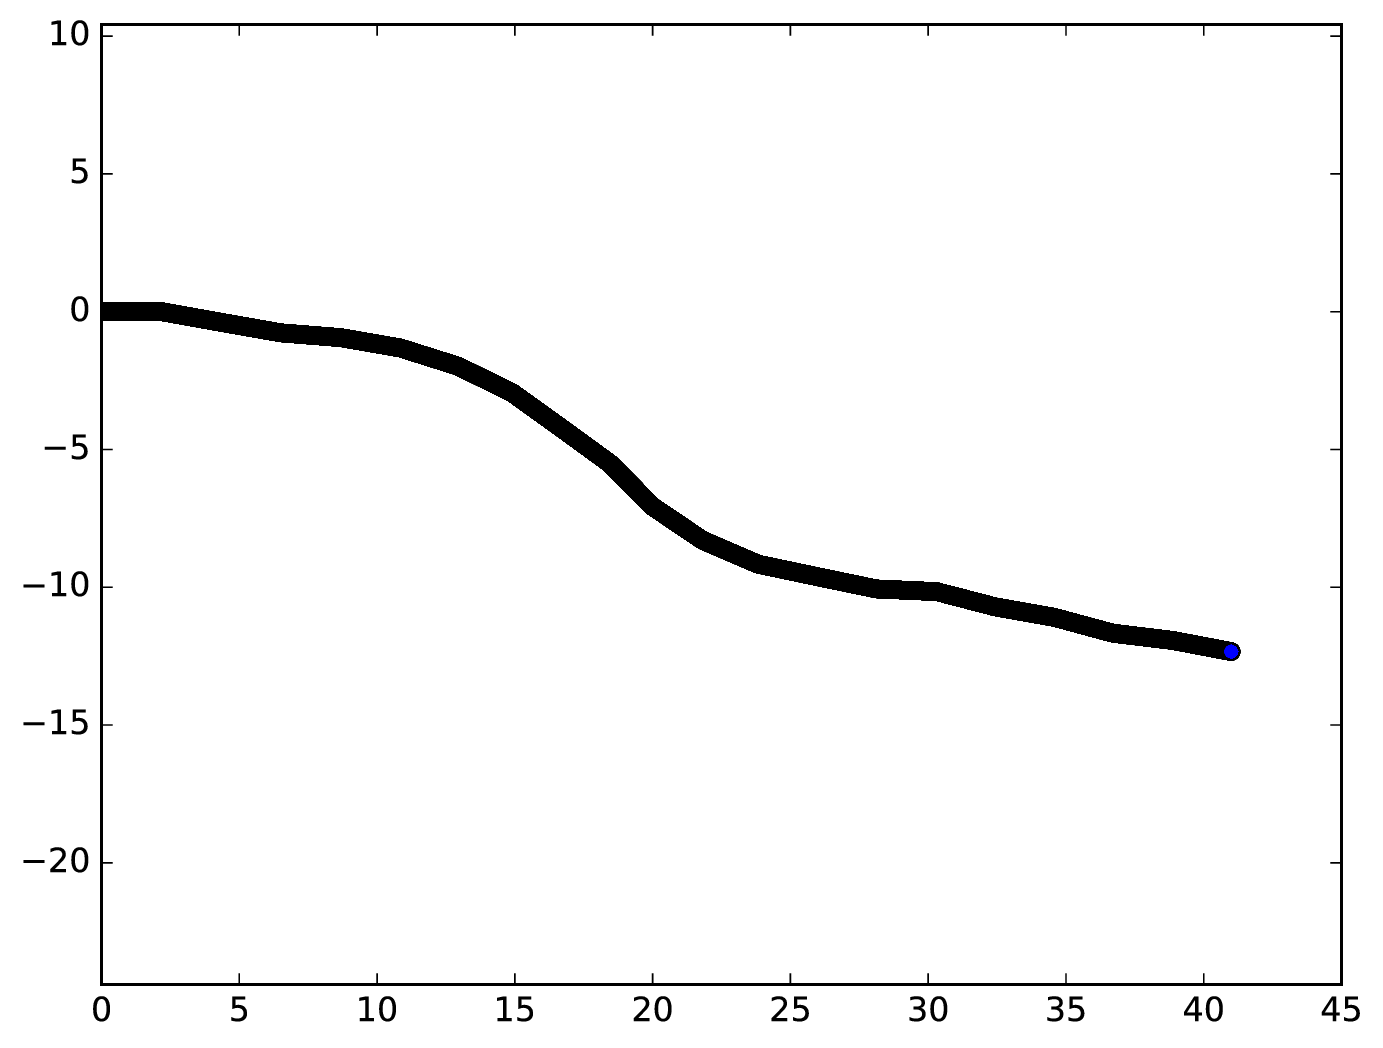
\includegraphics[width=\textwidth]{figures/ch3/synTraj_219_15_1}
			\caption[$A = 15$, $F=1$]{$A = 15$, $F=1$}
			\label{fig:synTraj_219_15_1}
		\end{subfigure}
		~
		\begin{subfigure}[t]{\subImgWmo}
			\centering
			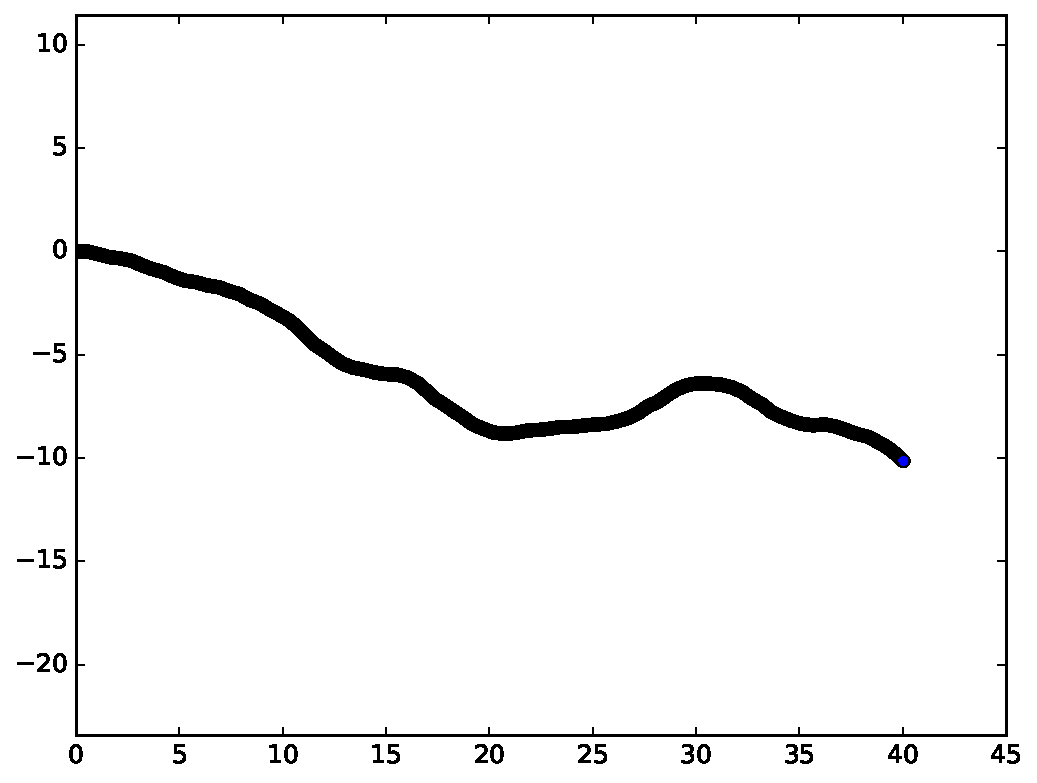
\includegraphics[width=\textwidth]{figures/ch3/synTraj_219_15_4}
			\caption[$A = 15$, $F=4$]{$A = 15$, $F=4$}
			\label{fig:synTraj_219_15_4}
		\end{subfigure}
		~
		\begin{subfigure}[t]{\subImgWmo}
			\centering
			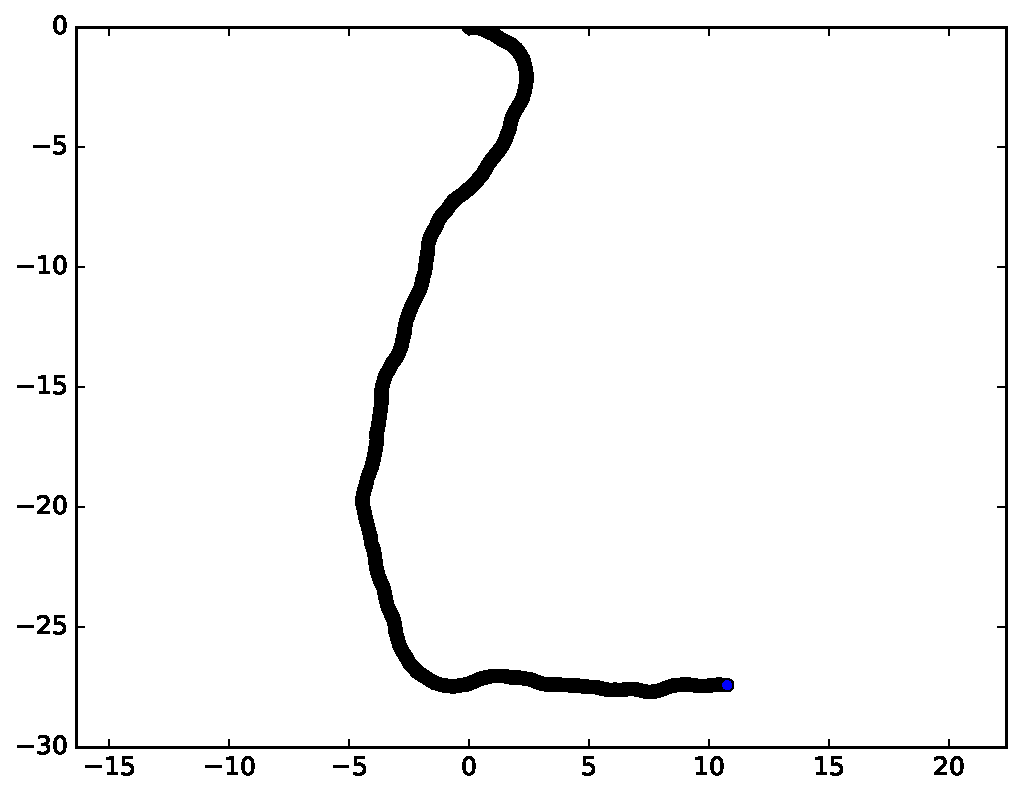
\includegraphics[width=\textwidth]{figures/ch3/synTraj_219_15_8}
			\caption[$A = 15$, $F=8$]{$A = 15$, $F=8$}
			\label{fig:synTraj_219_15_8}
		\end{subfigure}
		~
		\begin{subfigure}[t]{\subImgWmo}
			\centering
			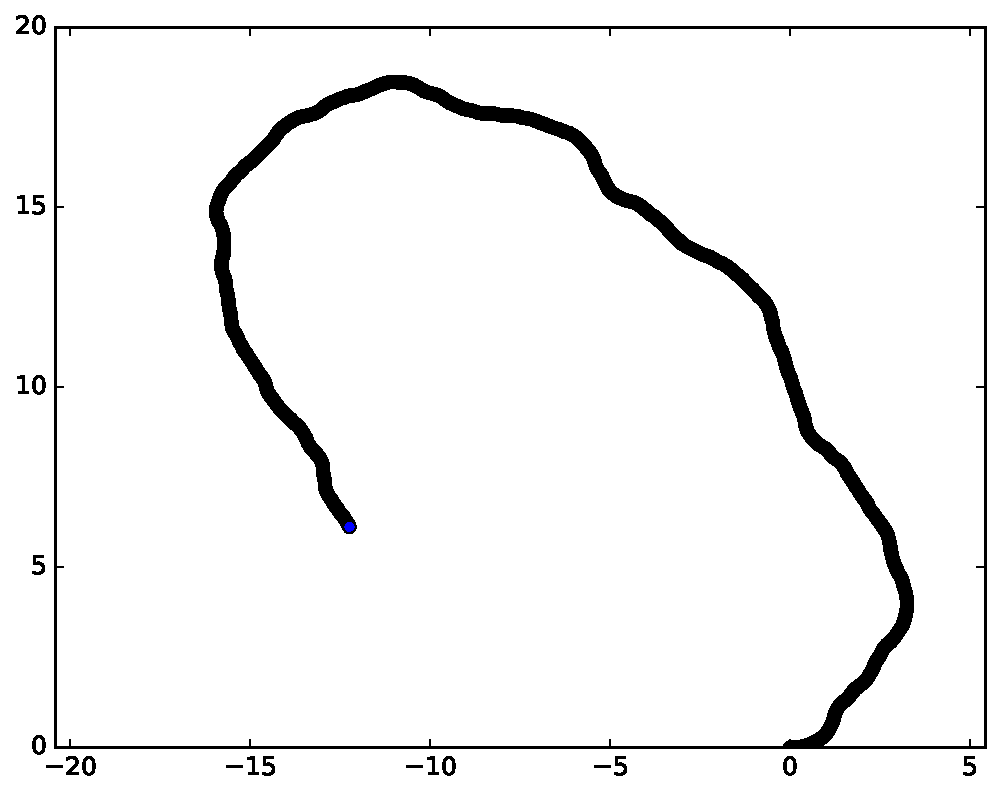
\includegraphics[width=\textwidth]{figures/ch3/synTraj_219_15_16}
			\caption[$A = 15$, $F=16$]{$A = 15$, $F=16$}
			\label{fig:synTraj_219_15_16}
		\end{subfigure}
		~
		\begin{subfigure}[t]{\subImgWmo}
			\centering
			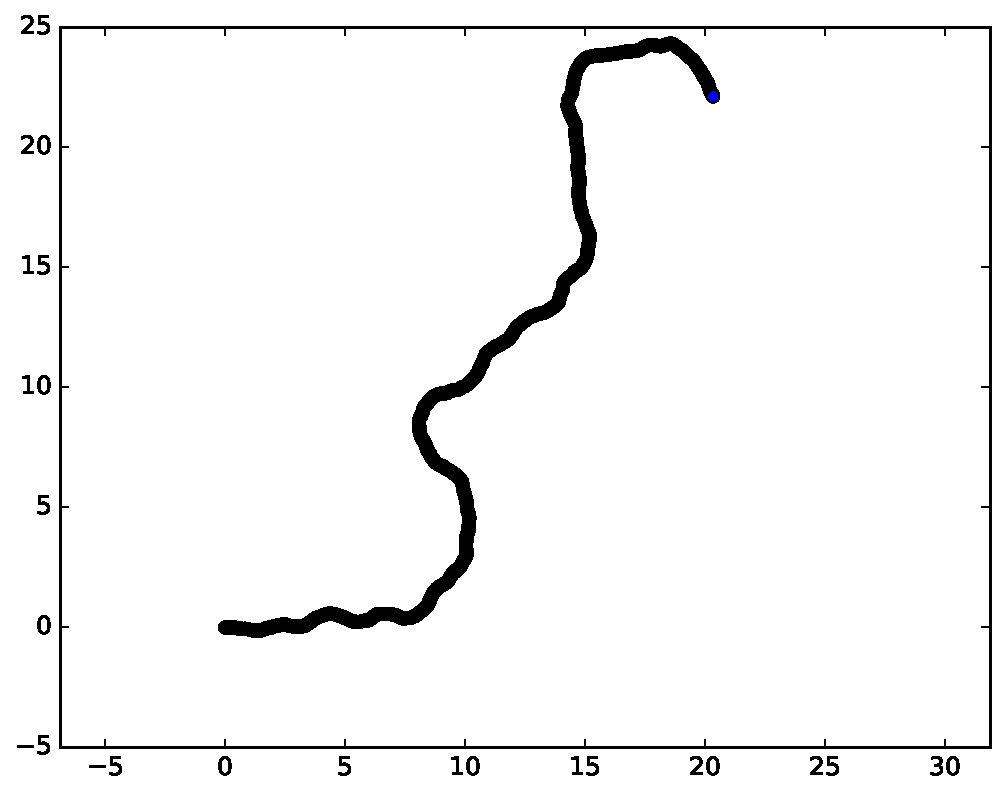
\includegraphics[width=\textwidth]{figures/ch3/synTraj_219_15_32}
			\caption[$A = 15$, $F=32$]{$A = 15$, $F=32$}
			\label{fig:synTraj_219_15_32}
		\end{subfigure}
		~
		\begin{subfigure}[t]{\subImgWmo}
			\centering
			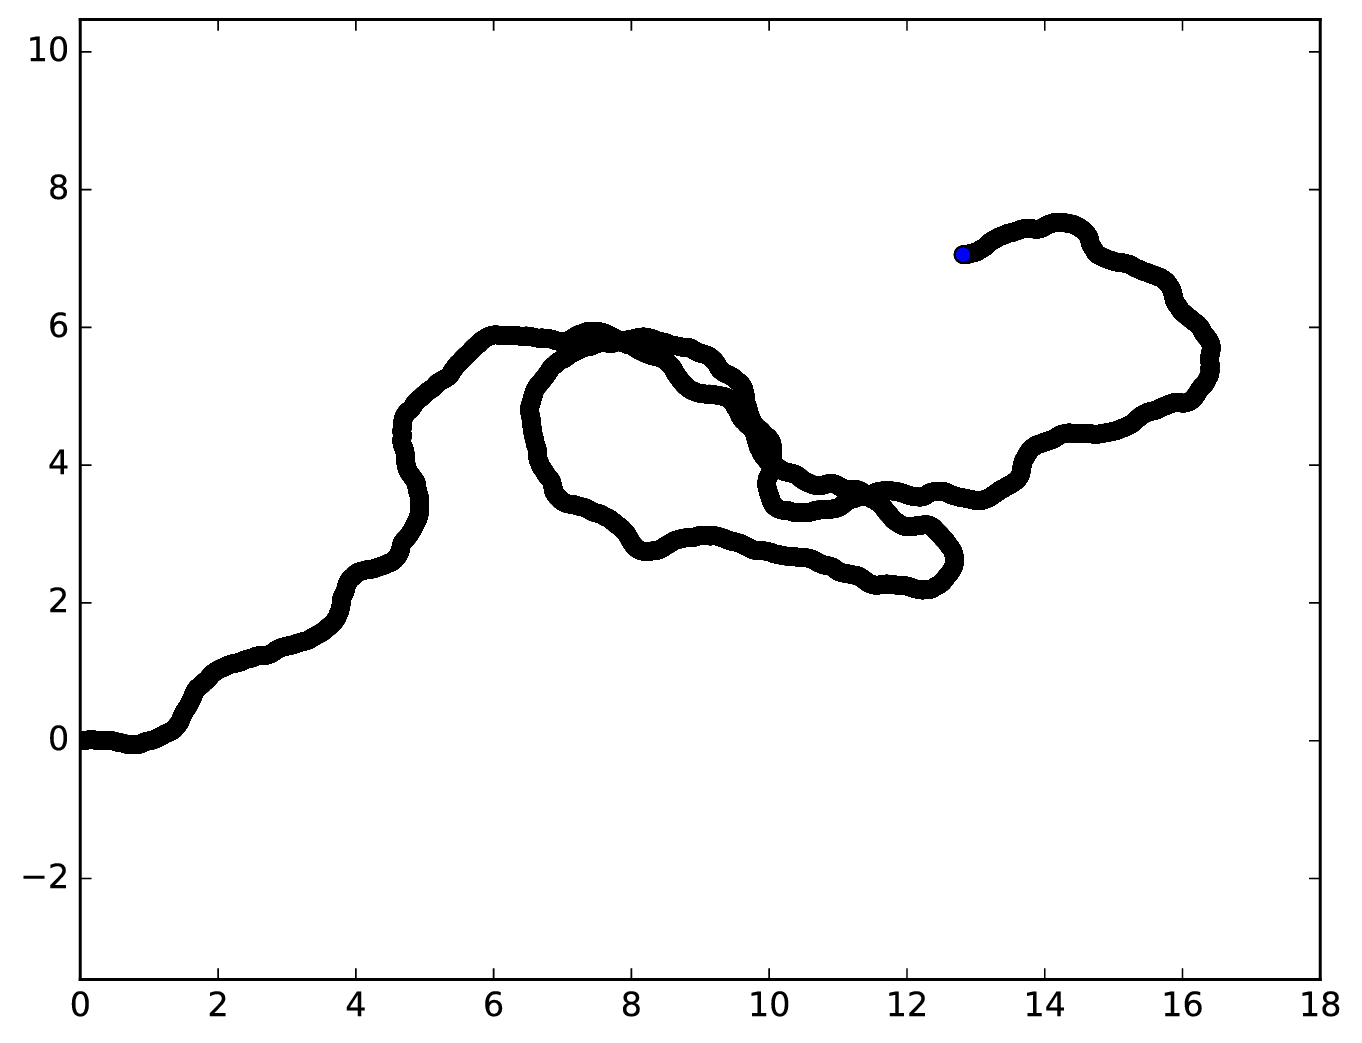
\includegraphics[width=\textwidth]{figures/ch3/synTraj_219_15_60}
			\caption[$A = 15$, $F=60$]{$A = 15$, $F=60$}
			\label{fig:synTraj_219_15_60}
		\end{subfigure}
		~
		\begin{subfigure}[t]{\subImgWmo}
			\centering
			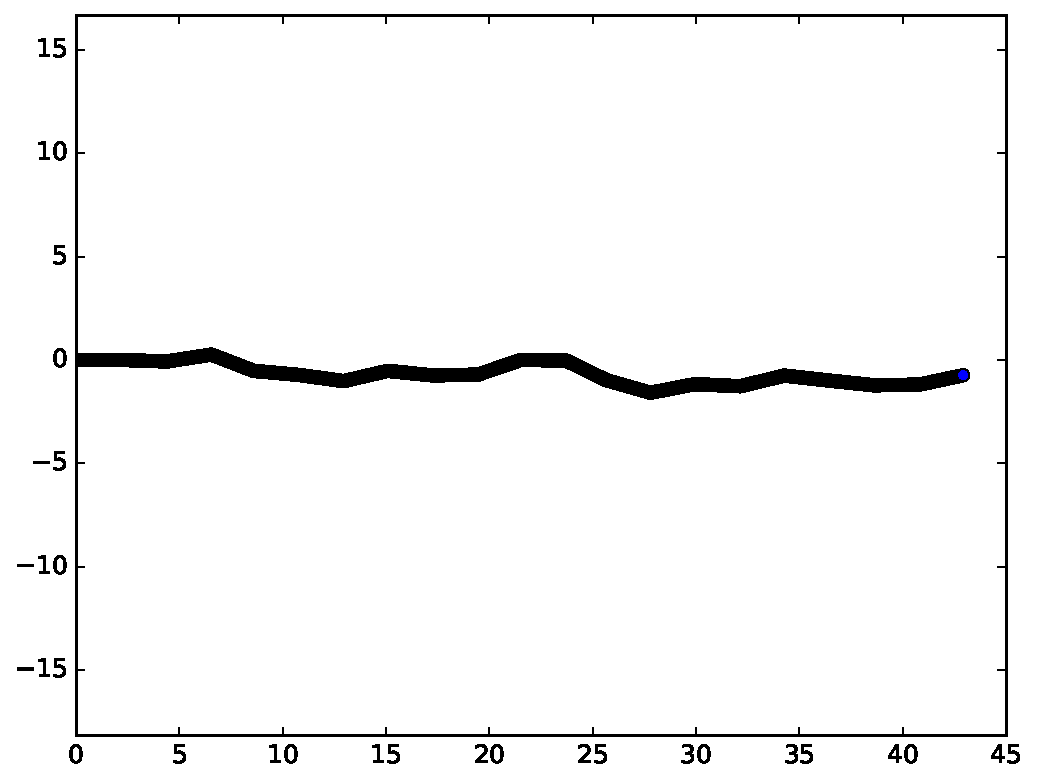
\includegraphics[width=\textwidth]{figures/ch3/synTraj_219_30_1}
			\caption[$A = 30$, $F=1$]{$A = 30$, $F=1$}
			\label{fig:synTraj_219_30_1}
		\end{subfigure}
		~
		\begin{subfigure}[t]{\subImgWmo}
			\centering
			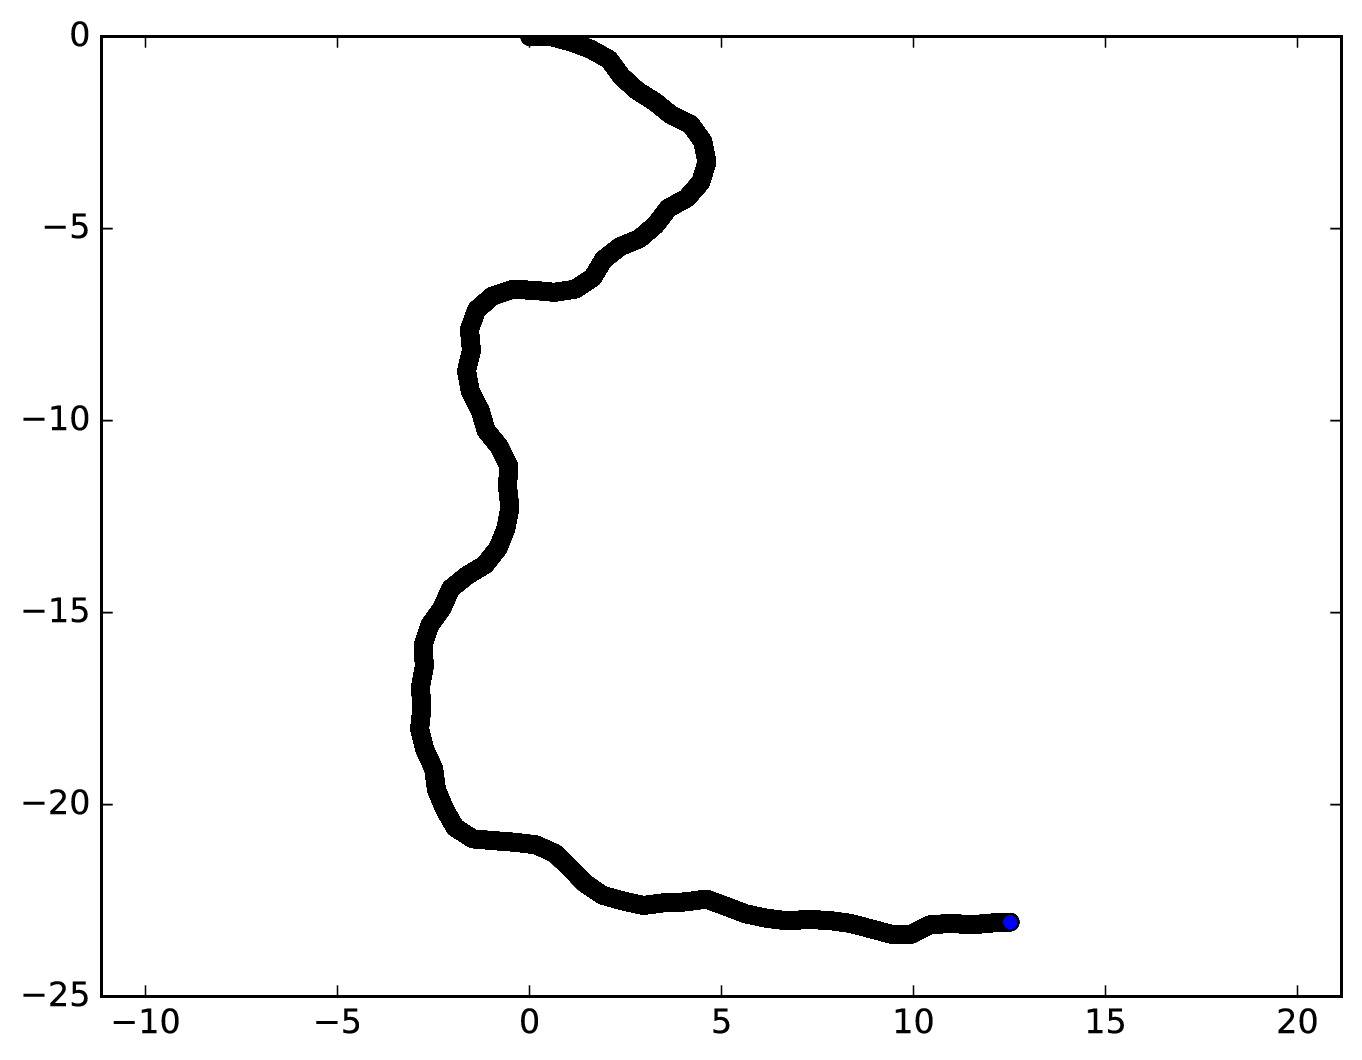
\includegraphics[width=\textwidth]{figures/ch3/synTraj_219_30_4}
			\caption[$A = 30$, $F=4$]{$A = 30$, $F=4$}
			\label{fig:synTraj_219_30_4}
		\end{subfigure}
		~
		\begin{subfigure}[t]{\subImgWmo}
			\centering
			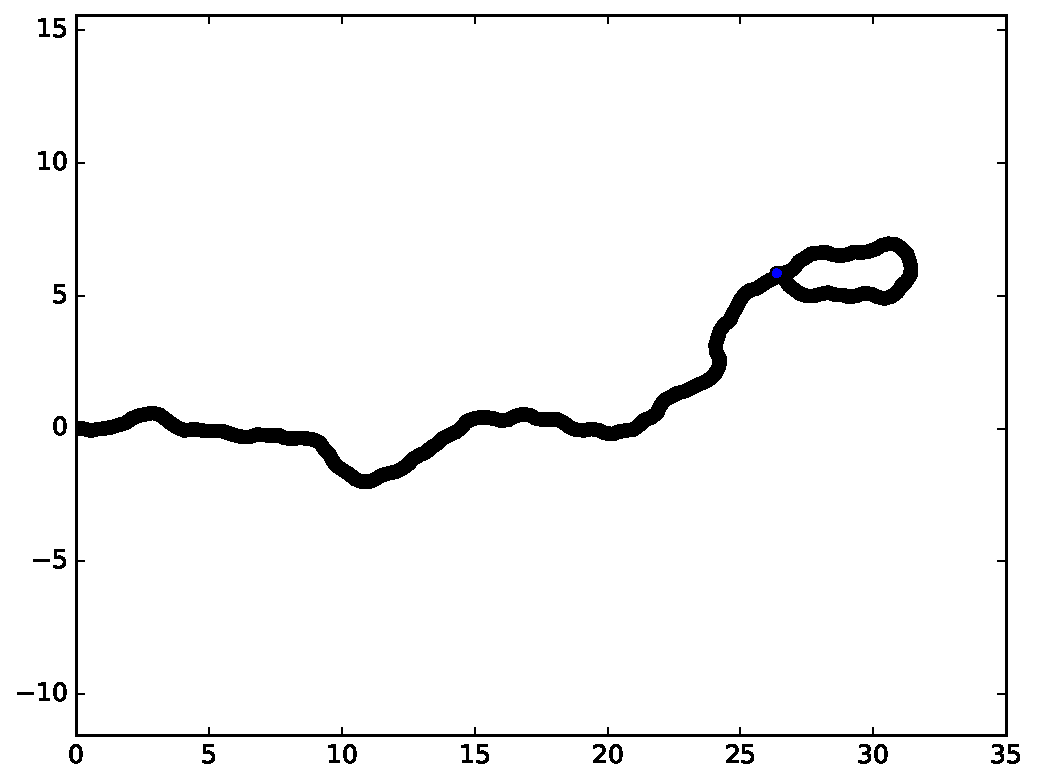
\includegraphics[width=\textwidth]{figures/ch3/synTraj_219_30_8}
			\caption[$A = 30$, $F=8$]{$A = 30$, $F=8$}
			\label{fig:synTraj_219_30_8}
		\end{subfigure}
		~
		\begin{subfigure}[t]{\subImgWmo}
			\centering
			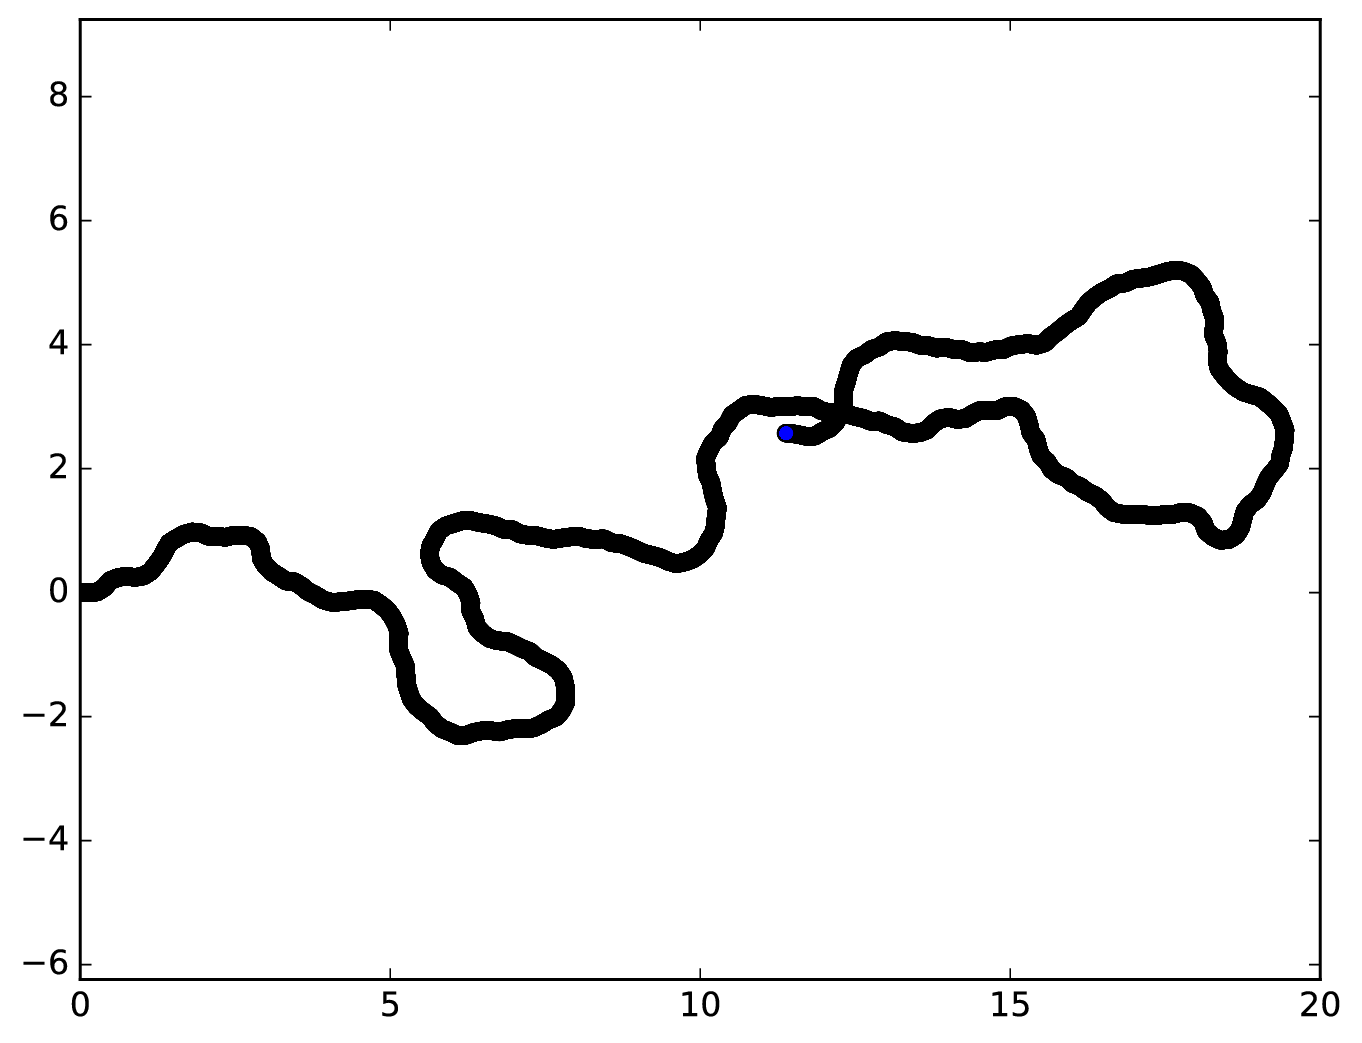
\includegraphics[width=\textwidth]{figures/ch3/synTraj_219_30_16}
			\caption[$A = 30$, $F=16$]{$A = 30$, $F=16$}
			\label{fig:synTraj_219_30_16}
		\end{subfigure}
		~
		\begin{subfigure}[t]{\subImgWmo}
			\centering
			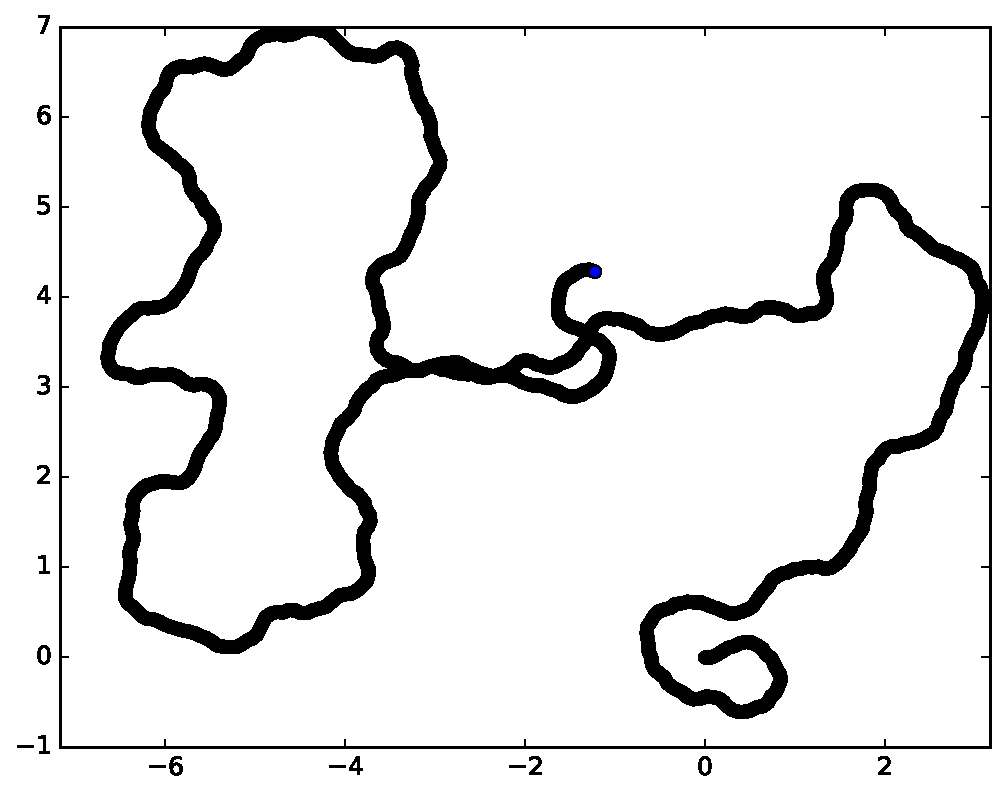
\includegraphics[width=\textwidth]{figures/ch3/synTraj_219_30_32}
			\caption[$A = 30$, $F=32$]{$A = 30$, $F=32$}
			\label{fig:synTraj_219_30_32}
		\end{subfigure}
		~
		\begin{subfigure}[t]{\subImgWmo}
			\centering
			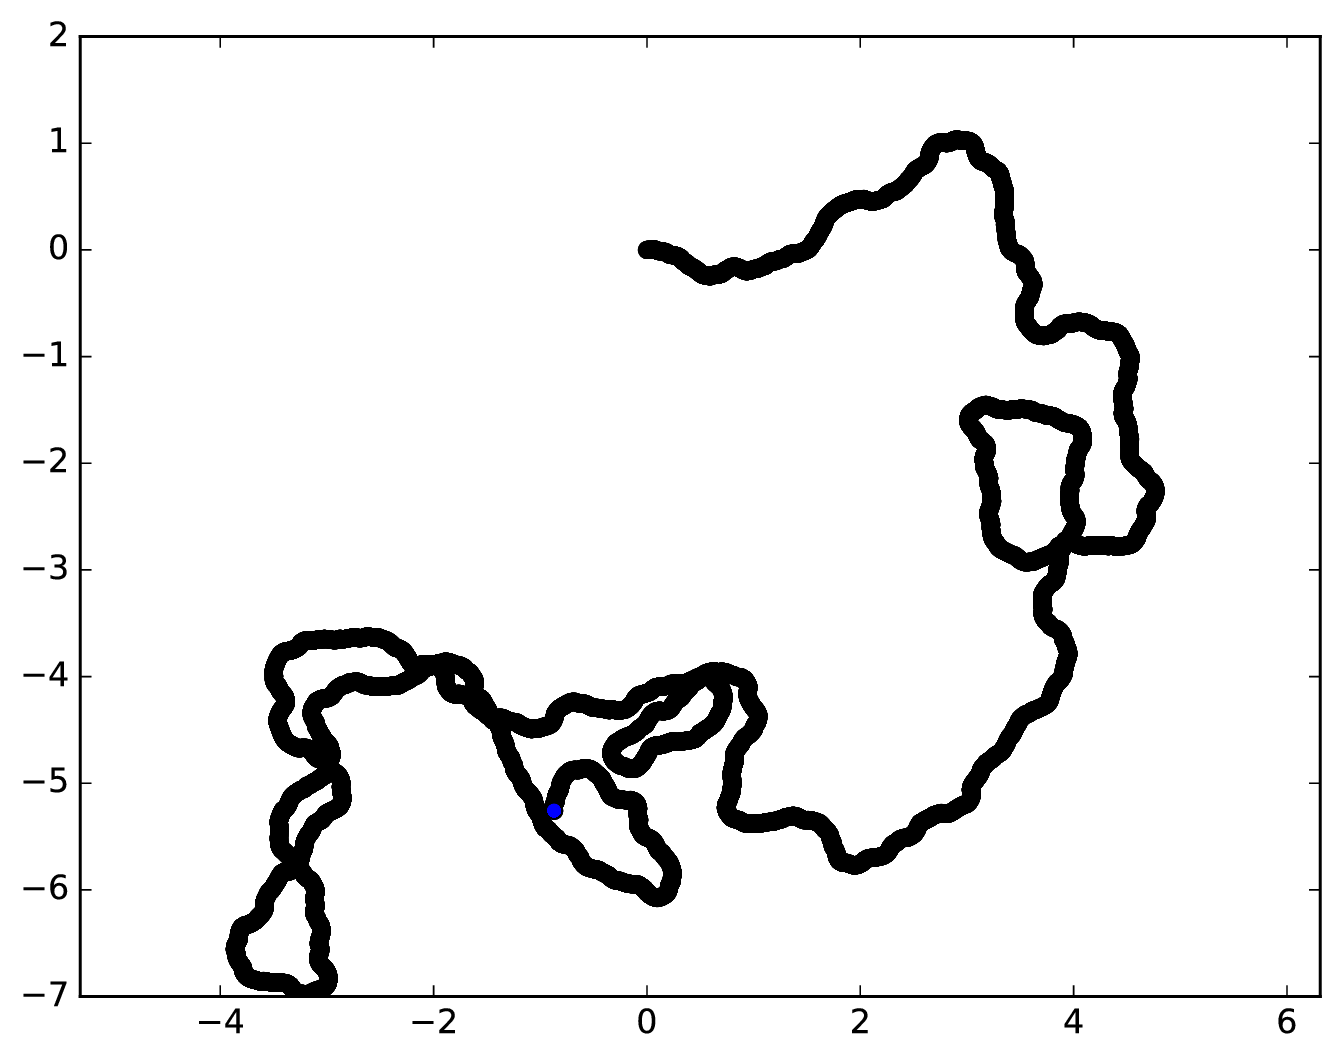
\includegraphics[width=\textwidth]{figures/ch3/synTraj_219_30_60}
			\caption[$A = 30$, $F=60$]{$A = 30$, $F=60$}
			\label{fig:synTraj_219_30_60}
		\end{subfigure}
		\caption[Mouvements générés par notre modèle]{Exemples de trajectoires générées par notre modèle pour un objet de vitesse constante (2,19~cm/s).}
		\label{fig:motion1530}
	\end{figure}
	
	\subsubsection{Mouvement pseudo-autocorrélé}
	On notera (notamment sur la figure~\ref{fig:motion1530}, et dans une moindre mesure sur les autres) que quand les valeurs de $A$ ou $F$ sont faibles, ou \emph{a fortiori} quand les deux le sont, le mouvement semble présenter une certaine régularité, au point peut-être de donner l'illusion d'être autocorrélé. La figure~\ref{fig:synTraj_219_45_1}, malgré sa valeur de $A$ relativement élevée, en fournit un exemple.
	
	Cette observation est intéressante en ce que ce modèle conçu pour les objets markoviens peut fournir une approximation du mouvement autocorrélé qui, dans certains cas, peut être suffisante. C'est particulièremnt vrai sur une fenêtre temporelle plus restreinte, limitée à quelques secondes tout au plus --- mais une telle fenêtre peut être trop courte pour certaines applications.
	
	À défaut d'être réellement autocorrélés, les mouvements générés par ces conditions (que l'on peut résumer par une valeur de $A \times F$ faible) engendrent des trajectoires suffisamment \og régulières \fg{} pour être relativement prévisibles à court terme (sur une ou deux secondes). Nous reviendrons plus loin sur l'importance de la prévisibilité pour une tâche de sélection. Contentons-nous pour le moment de remarquer qu'un objet dont les changements de direction sont rares et/ou de faible amplitude tend à avoir une trajectoire relativement \og lisse \fg{} et, de fait, prévisible.


	\begin{figure}[htb]
		\begin{subfigure}[t]{\subImgWmo}
			\centering
			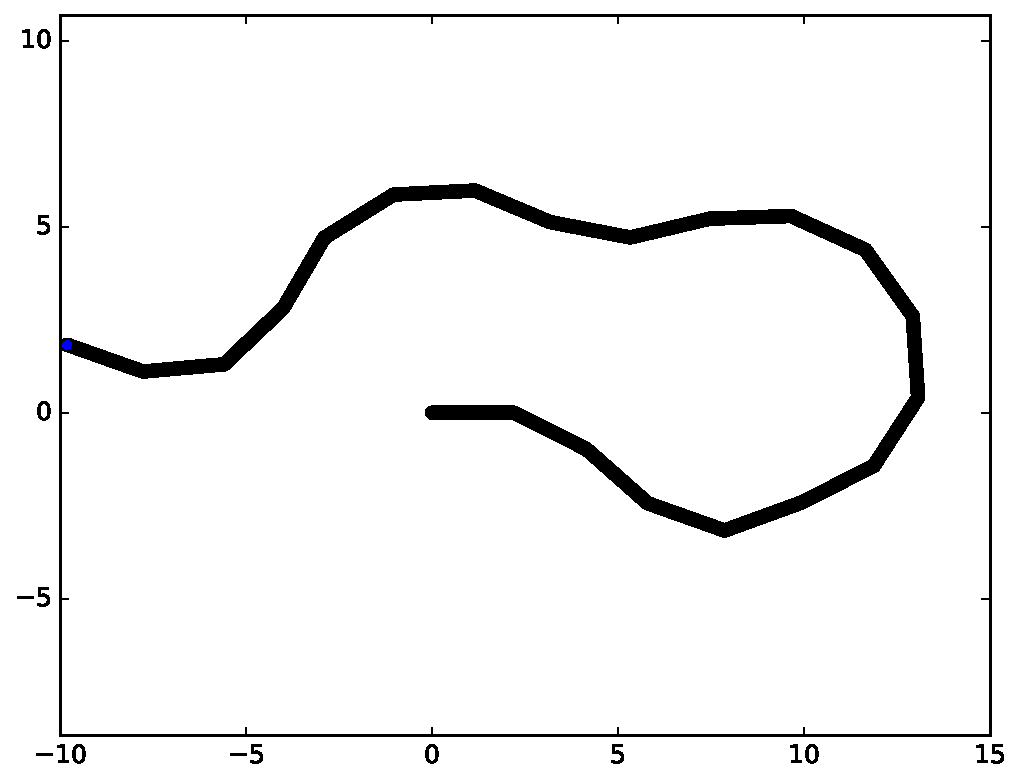
\includegraphics[width=\textwidth]{figures/ch3/synTraj_219_45_1}
			\caption[$A = 45$, $F=1$]{$A = 45$, $F=1$}
			\label{fig:synTraj_219_45_1}
		\end{subfigure}
		~
		\begin{subfigure}[t]{\subImgWmo}
			\centering
			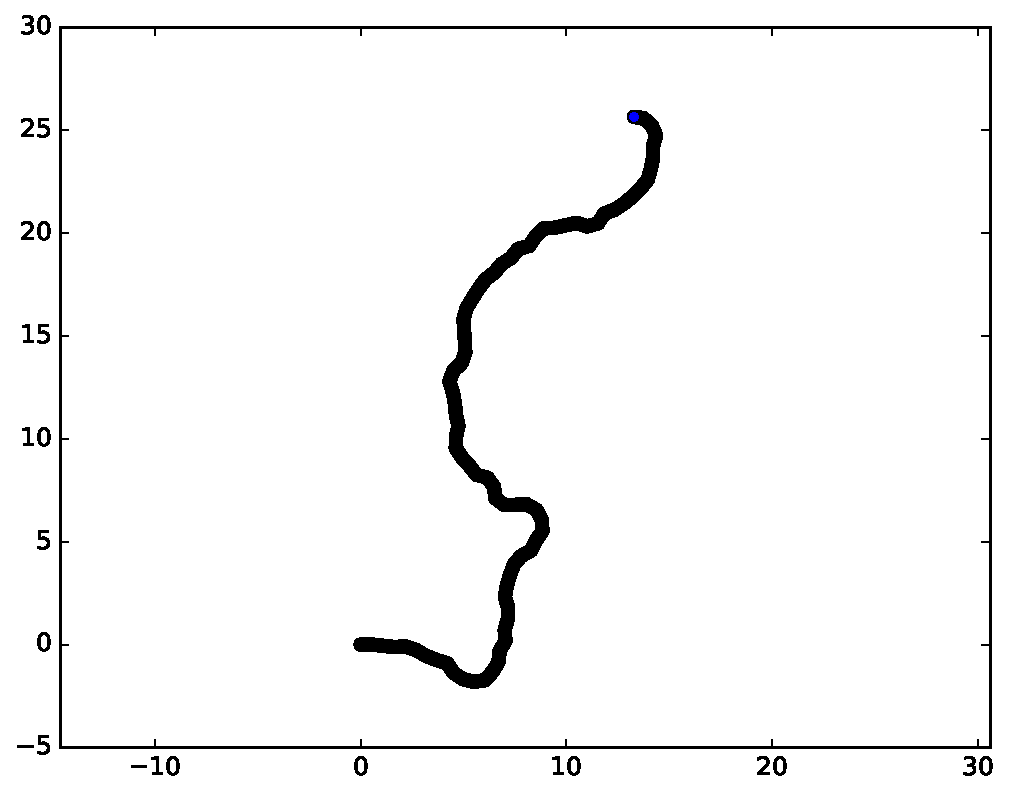
\includegraphics[width=\textwidth]{figures/ch3/synTraj_219_45_4}
			\caption[$A = 45$, $F=4$]{$A = 45$, $F=4$}
			\label{fig:synTraj_219_45_4}
		\end{subfigure}
		~
		\begin{subfigure}[t]{\subImgWmo}
			\centering
			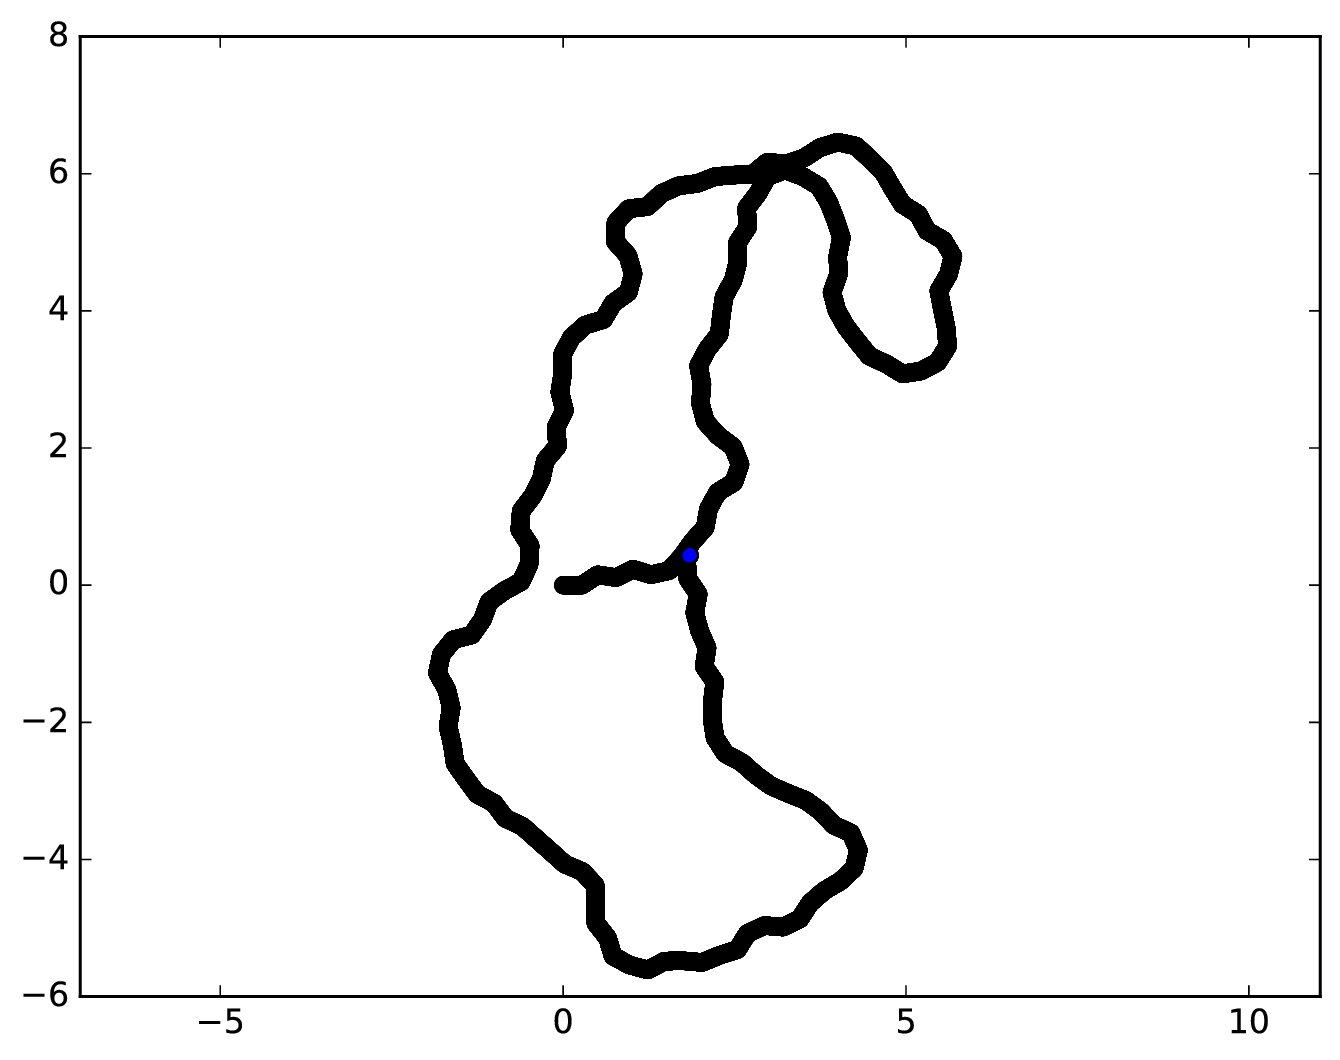
\includegraphics[width=\textwidth]{figures/ch3/synTraj_219_45_8}
			\caption[$A = 45$, $F=8$]{$A = 45$, $F=8$}
			\label{fig:synTraj_219_45_8}
		\end{subfigure}
		~
		\begin{subfigure}[t]{\subImgWmo}
			\centering
			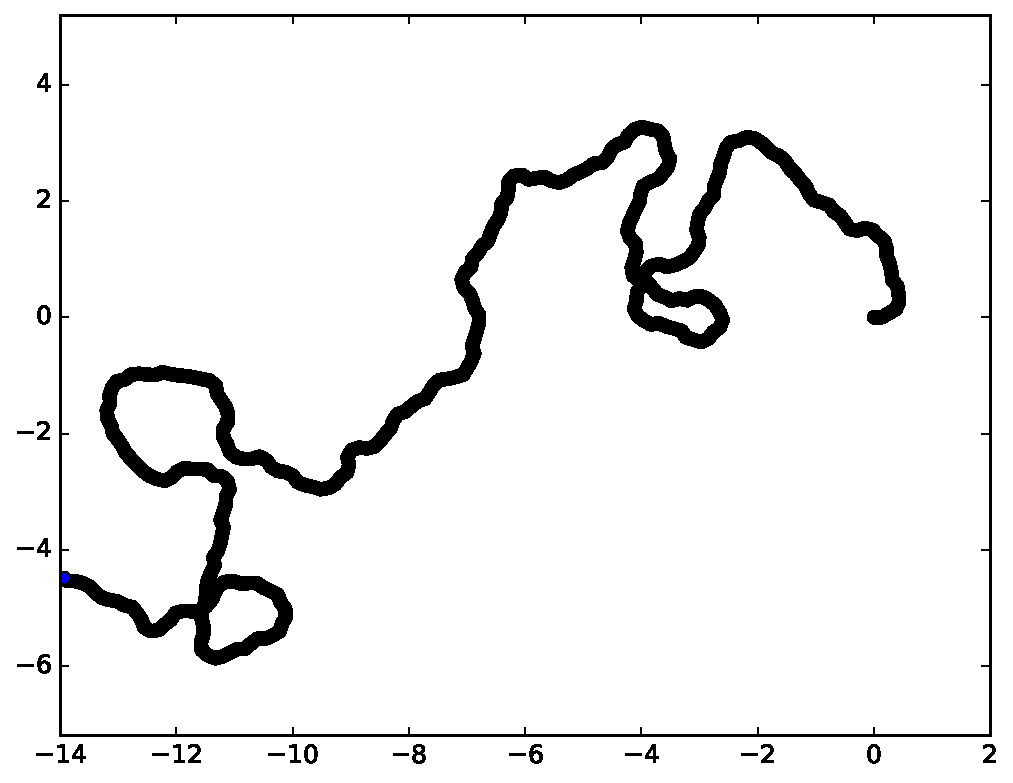
\includegraphics[width=\textwidth]{figures/ch3/synTraj_219_45_16}
			\caption[$A = 45$, $F=16$]{$A = 45$, $F=16$}
			\label{fig:synTraj_219_45_16}
		\end{subfigure}
		~
		\begin{subfigure}[t]{\subImgWmo}
			\centering
			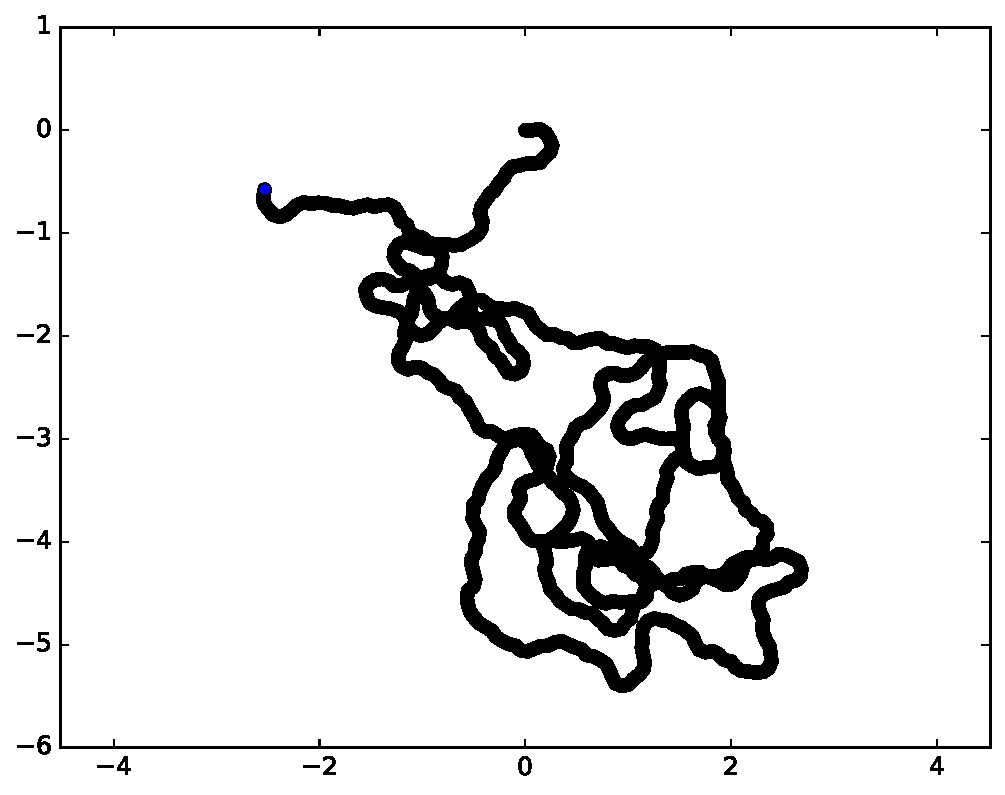
\includegraphics[width=\textwidth]{figures/ch3/synTraj_219_45_32}
			\caption[$A = 45$, $F=32$]{$A = 45$, $F=32$}
			\label{fig:synTraj_219_45_32}
		\end{subfigure}
		~
		\begin{subfigure}[t]{\subImgWmo}
			\centering
			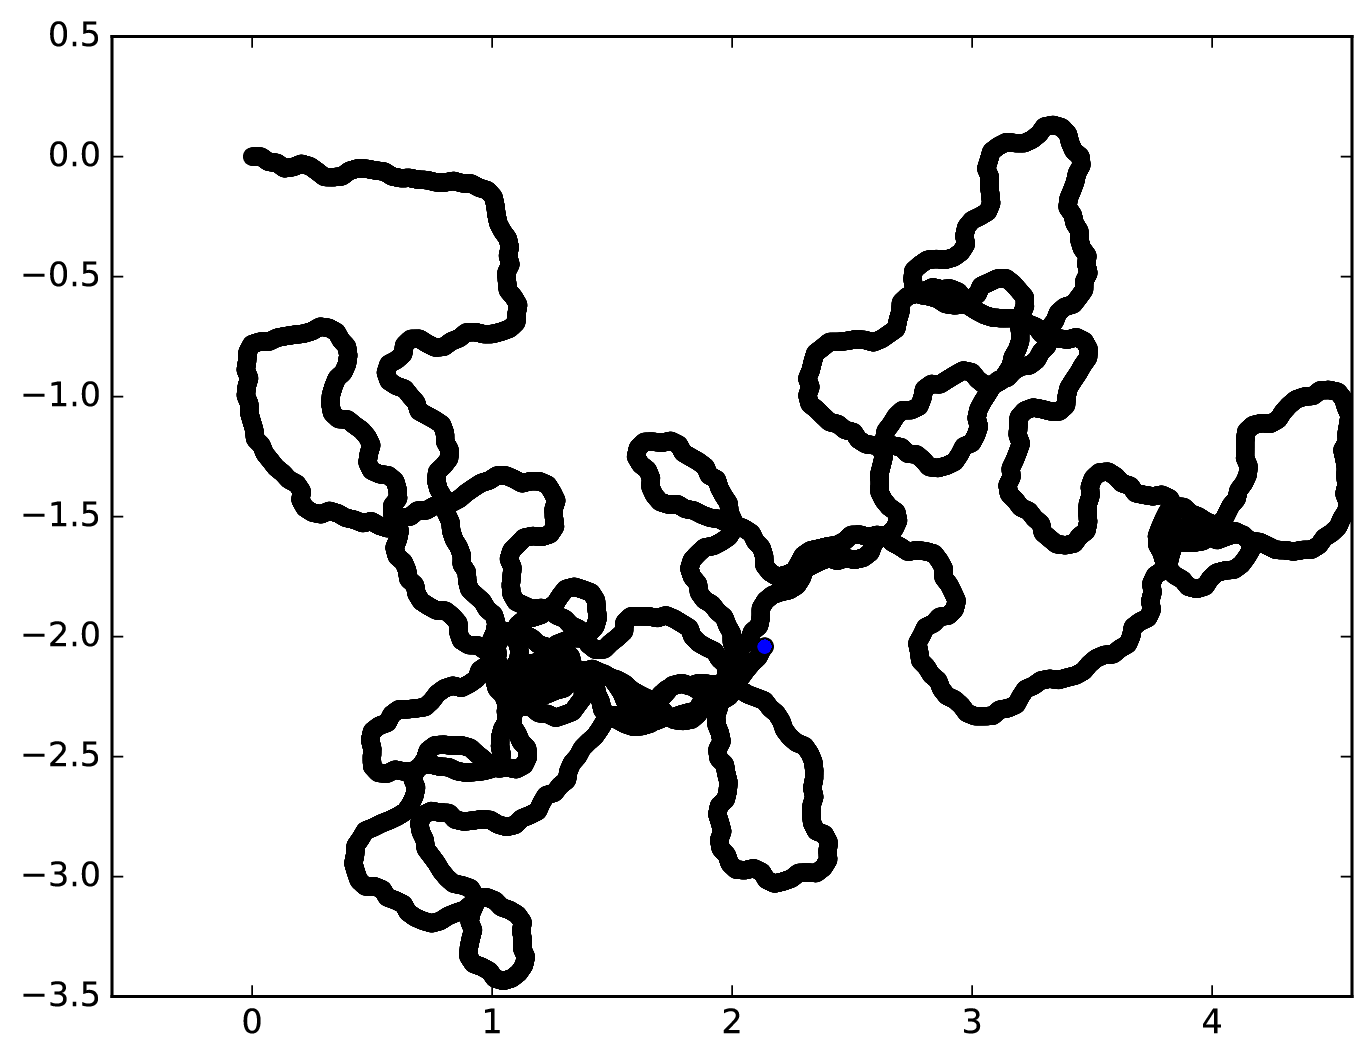
\includegraphics[width=\textwidth]{figures/ch3/synTraj_219_45_60}
			\caption[$A = 45$, $F=60$]{$A = 45$, $F=60$}
			\label{fig:synTraj_219_45_60}
		\end{subfigure}
		~
		\begin{subfigure}[t]{\subImgWmo}
			\centering
			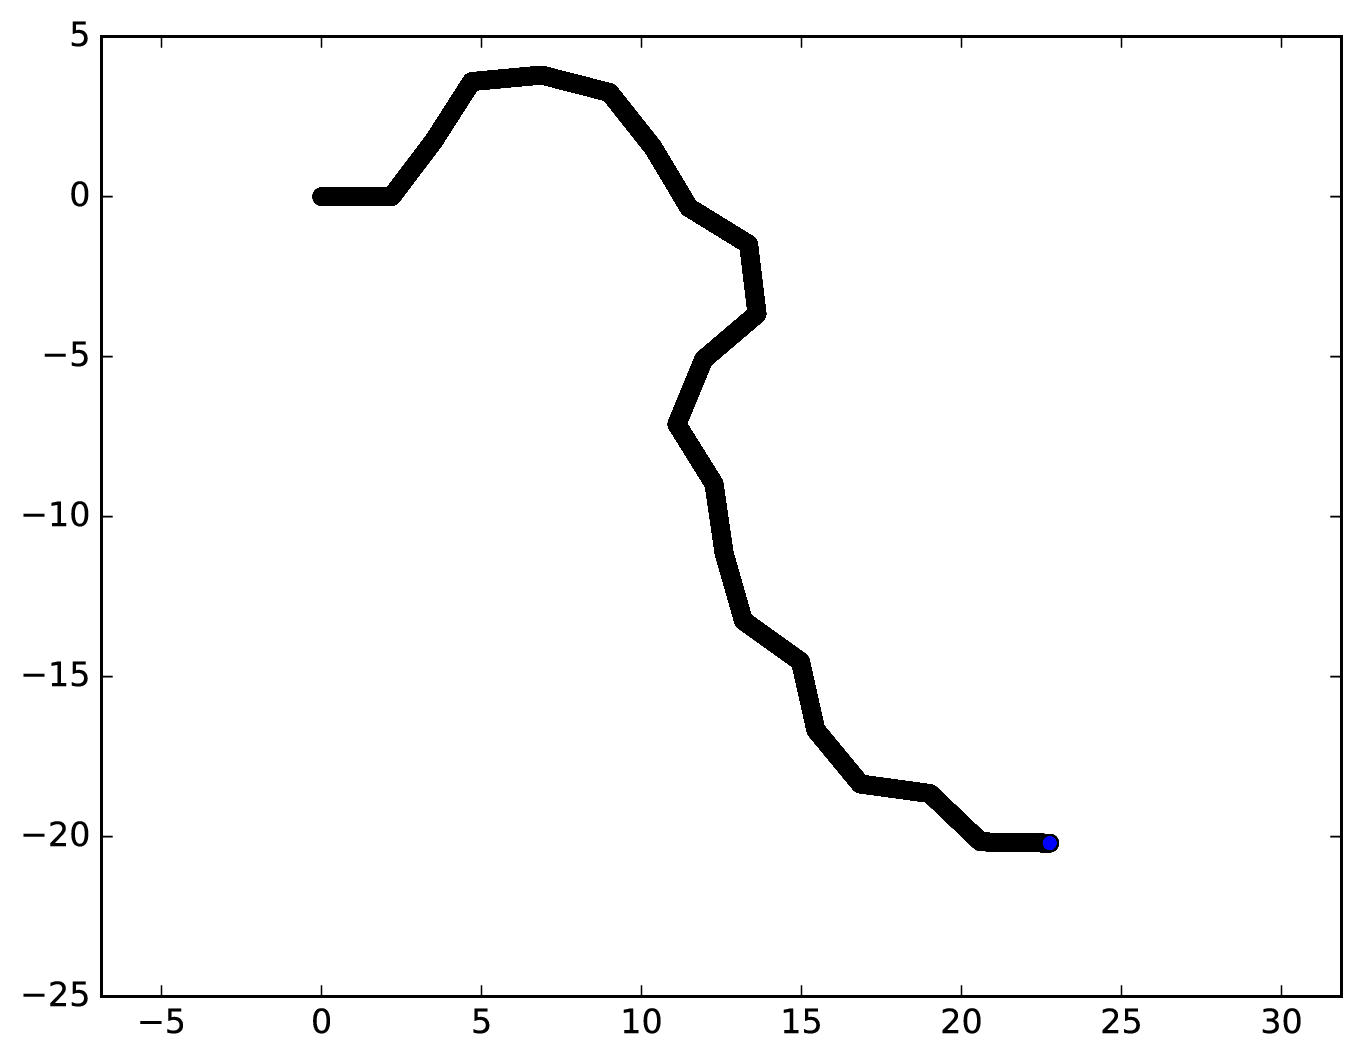
\includegraphics[width=\textwidth]{figures/ch3/synTraj_219_60_1}
			\caption[$A = 60$, $F=1$]{$A = 60$, $F=1$}
			\label{fig:synTraj_219_60_1}
		\end{subfigure}
		~
		\begin{subfigure}[t]{\subImgWmo}
			\centering
			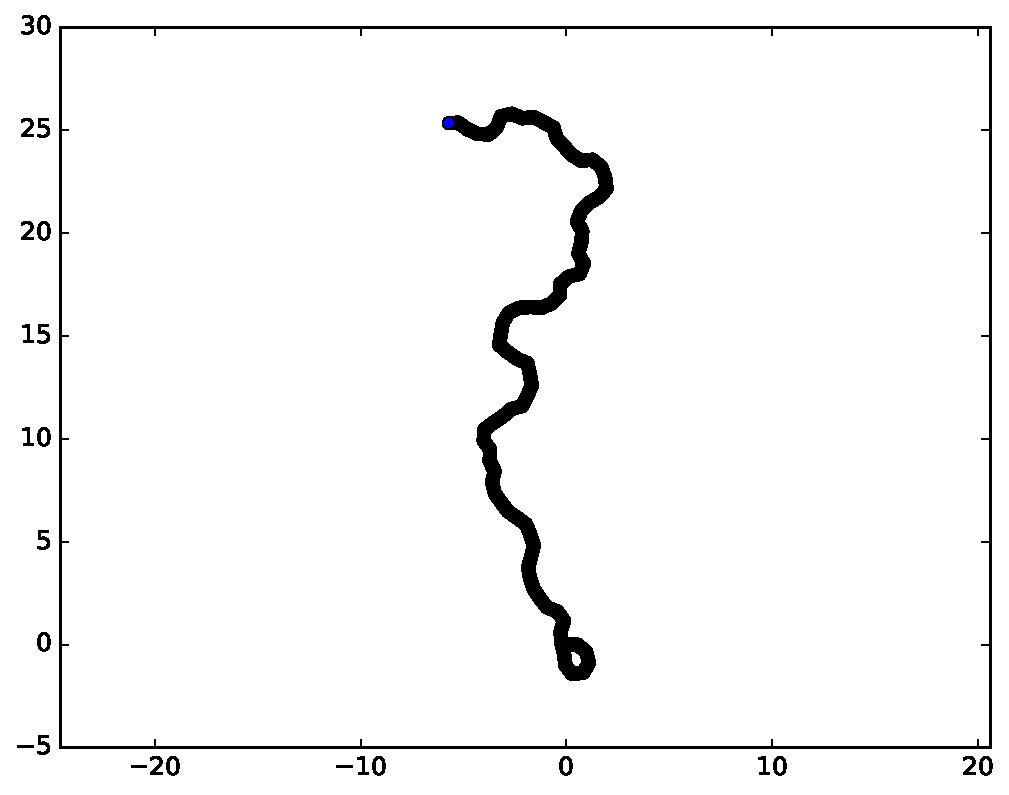
\includegraphics[width=\textwidth]{figures/ch3/synTraj_219_60_4}
			\caption[$A = 60$, $F=4$]{$A = 60$, $F=4$}
			\label{fig:synTraj_219_60_4}
		\end{subfigure}
		~
		\begin{subfigure}[t]{\subImgWmo}
			\centering
			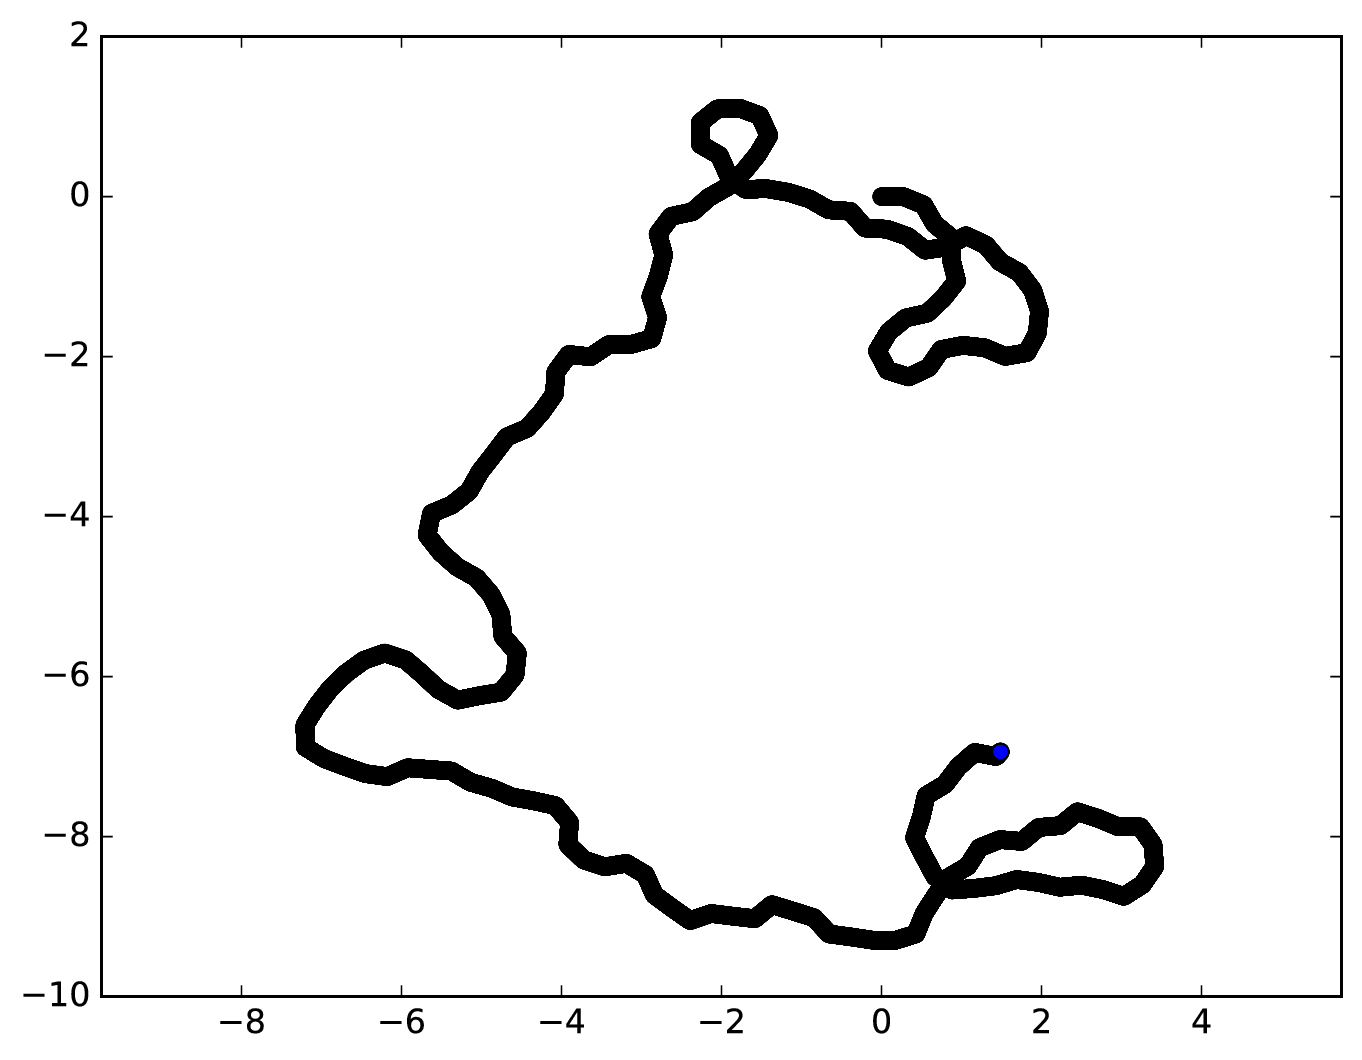
\includegraphics[width=\textwidth]{figures/ch3/synTraj_219_60_8}
			\caption[$A = 60$, $F=8$]{$A = 60$, $F=8$}
			\label{fig:synTraj_219_60_8}
		\end{subfigure}
		~
		\begin{subfigure}[t]{\subImgWmo}
			\centering
			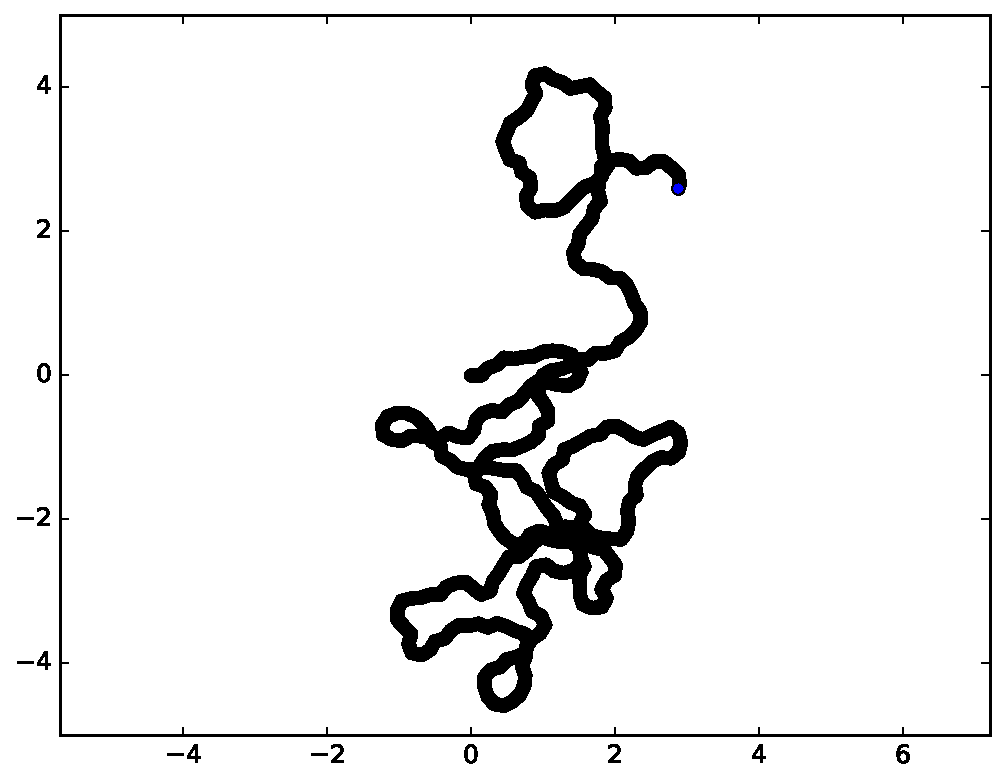
\includegraphics[width=\textwidth]{figures/ch3/synTraj_219_60_16}
			\caption[$A = 60$, $F=16$]{$A = 60$, $F=16$}
			\label{fig:synTraj_219_60_16}
		\end{subfigure}
		~
		\begin{subfigure}[t]{\subImgWmo}
			\centering
			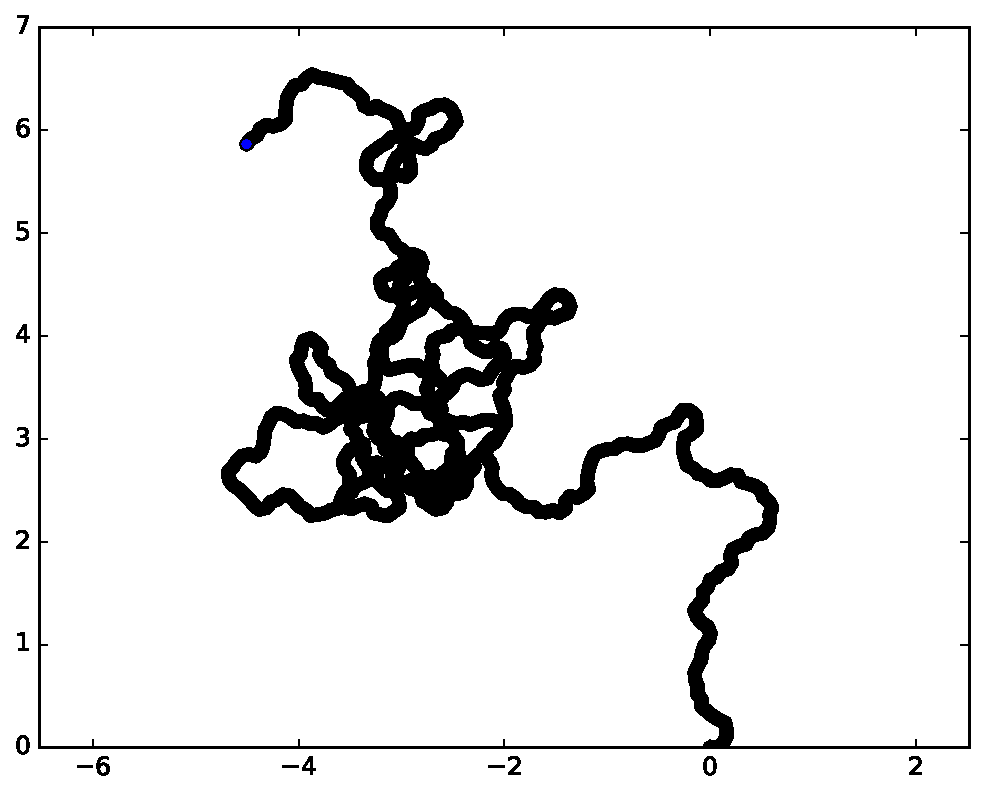
\includegraphics[width=\textwidth]{figures/ch3/synTraj_219_60_32}
			\caption[$A = 60$, $F=32$]{$A = 60$, $F=32$}
			\label{fig:synTraj_219_60_32}
		\end{subfigure}
		~
		\begin{subfigure}[t]{\subImgWmo}
			\centering
			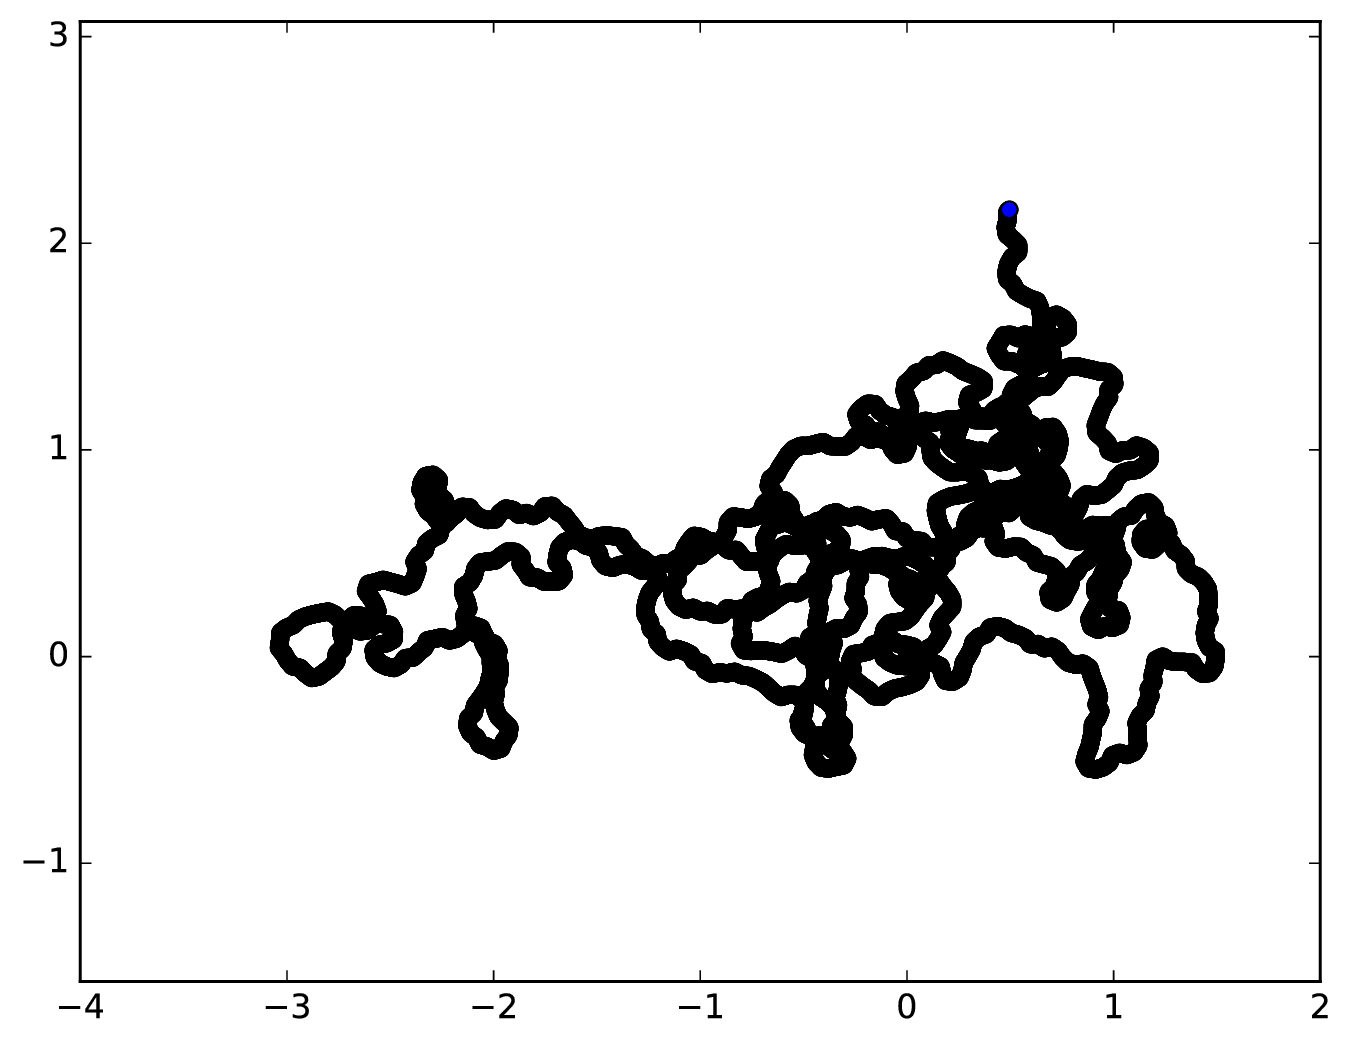
\includegraphics[width=\textwidth]{figures/ch3/synTraj_219_60_60}
			\caption[$A = 60$, $F=60$]{$A = 60$, $F=60$}
			\label{fig:synTraj_219_60_60}
		\end{subfigure}
		\caption[Mouvements générés par notre modèle -- II]{Exemples de trajectoires générées par notre modèle pour un objet de vitesse constante (2,19~cm/s).}
		\label{fig:motion4560}
	\end{figure}
	
	\subsubsection{Entropie}
	Dans ses travaux sur la thermodynamique, Rudolf Clausius définit l'entropie comme \og le contenu de tranformation [d'un] corps \fg{}~\cite{clausius1865verschiedene, clausius1865diverses}. Rapidement, Ludwig Boltzmann redéfinit l'entropie $S$ par l'équation $S = k\log(W)$, où $k$ est une constante et $W$ est le nombre d'états dans lequel un système peut se trouver~\cite{boltzmann1866mechanische, weisstein2004eric}.
	
	À partir de la définition de Boltzmann, Claude Shannon redéfinit à nouveau l'entropie~\cite{shannon1949communication} (qu'il préfère noter $H(X)$) d'une variable aléatoire discrète $X$ de valeurs possibles $\{x_{1}, \ldots{}, x_{n}\}$ par l'équation~\ref{eq:shannonEntropy}, où $P(x_{i})$ est la probabilité que $X=x_{i}$.
	
	\begin{equation}
		\label{eq:shannonEntropy}
		H(X) = -\sum_{i=1}^{n}P(x_{i})\log_{b}\left(P(x_{i})\right)
	\end{equation}
	
	L'on peut toutefois écrire cette équation de façon plus succincte --- et peut-être plus parlante --- comme dans l'équation~\ref{eq:shaEnt}, où $I(X)$ est la quantité d'information de $X$, et $E[I(X)]$ est l'espérance de cette quantité. Notez que $I(e) = -\log\left(P(e)\right)$, où $e$ est un événement.
	
	\begin{equation}
		\label{eq:shaEnt}
		H(X) = E[I(X)]
	\end{equation}
	
	En résumé, pour Shannon, l'entropie d'une variable croît avec sa quantité d'information, et celle-ci est d'autant plus grande que les événements possibles sont rares. Si l'on suppose qu'ils sont équiprobables, alors ils sont d'autant plus rares qu'ils sont nombreux.
	
	Dans le cas qui nous concerne, on peut donc dire qu'une cible est de forte entropie si, pour une position donnée à l'instant $t$, les positions possibles à l'instant $t+1$ sont nombreuses (en les supposant équiprobables).
	
	Supposons donc une cible de position $pos$ et de vecteur direction $\vec{dir}$ à l'instant $t$. Si $F=0$ ou $A=0$, alors $pos_{t+1} = pos + S \times \vec{dir}$. Seul cet état est possible, donc la quantité d'information de la cible est nulle, et son entropie aussi. En revanche, s'il peut y avoir une rotation de $\vec{dir}$ à l'instant $t+1$, alors l'entropie sera non nulle, et dépendra de la probabilité de ce changement de direction, ainsi que du nombre de valeurs possibles pour le changement de direction $\alpha$.
	
	Si l'on considère $\alpha$ comme un nombre réel, en toute rigueur, le nombre de valeurs possibles est infini, et l'entropie aussi. L'on peut cependant considérer que pour un utilisateur, un changement de direction de 10,0001\textdegree{} ne sera généralement pas différent d'un changement de 10\textdegree{} ; aussi serait-il judicieux de discrétiser l'espace de $\alpha$. Une solution simple consiste à arrondir la valeur à l'entier le plus proche, ce qui réduit l'espace aux entiers contenus dans l'intervalle $[-180\degree{}, +180\degree{}]$, soit 360 valeurs (car $180 \equiv -180 \mod 360$).
	
	La portion de cet espace effectivement possible dépend de $A$ ; plus précicément, elle vaut $\frac{A}{180}$. L'on peut donc calculer l'entropie d'une cible si l'on connaît $A$ et si l'on sait qu'il y aura un changement de direction à l'instant suivant, mais ce calcul ne vaudra que sur une fenêtre temporelle limitée à deux \og instants \fg{} --- ce qui implique d'ailleurs une discrétisation du temps, potentiellement indésirable.
	
	Pour connaître l'entropie globale $E_{g}$ de la cible, on peut poser que $E_{g}$ est la moyenne des $E_{t}$ pour chaque instant $t$. Si l'on suppose que le temps est discrétisé de telle manière qu'un instant vaut $\frac{1}{60}$~s, alors $E_{g} = E_{t_{c}} \frac{F}{60}$ où $E_{t_{c}}$ est l'entropie de la cible à l'instant d'un changement de direction sûr.
	
	\paragraph{Pseudo-entropie.}
	Or, ce calcul d'entropie dépend d'hypothèses parfois très fortes :
	
	\begin{itemize}
		\item $A$ est connue ;
		\item $F$ est connu ;
		\item Pour une valeur de $A$ donnée, tous les $\alpha$ sont équiprobables ;
		\item La discrétisation de l'espace des $\alpha$ ne fausse pas l'estimation de l'entropie, c'est-à-dire qu'elle n'est ni trop fine ni trop grossière ;
		\item La discrétisation du temps ne fausse pas l'estimation de l'entropie, c'est-à-dire qu'elle n'est ni trop fine ni trop grossière.
	\end{itemize}
	
	Pour simplifier le problème, l'on peut simplement remarquer que :
	\begin{itemize}
		\item Plus $F$ est élevé, plus la direction change souvent,
		\item Plus $A$ est élevé, plus ces changements peuvent être importants,
		\item Les trajectoires observées sur les figures~\ref{fig:motion1530}, \ref{fig:motion4560}, \ref{fig:motion7590}, \ref{fig:motion105120}, \ref{fig:motion135150} et \ref{fig:motion165180} révèlent que, souvent, une trajectoire avec une valeur de $A$ relativement basse et une valeur de $F$ relativement haute sera subjectivement semblable à une trajectoire avec une valeur de $A$ relativement haute et une valeur de $F$ relativement basse.
	\end{itemize}
	
	Il paraît donc raisonnable d'envisager le produit $AF$ comme une pseudo-entropie, et ce d'autant plus qu'il s'annule dès lors que $A=0$ ou $F=0$, de même que l'entropie. Il a en outre le mérite d'être très simple à calculer, d'autant que ce calcul est possible à partir de valeurs typiques et maximales estimées.
	
	Nous pouvons aisément déduire des observations faites plus haut sur la fréquence des changements de direction et leurs amplitudes que l'entropie et la pseudo-entropie pourront être très élevées pour les objets ciné-discrets mais tendront à être faibles pour les objets ciné-continus (après discrétisation).
	
	\begin{figure}[htb]
		\begin{subfigure}[t]{\subImgWmo}
			\centering
			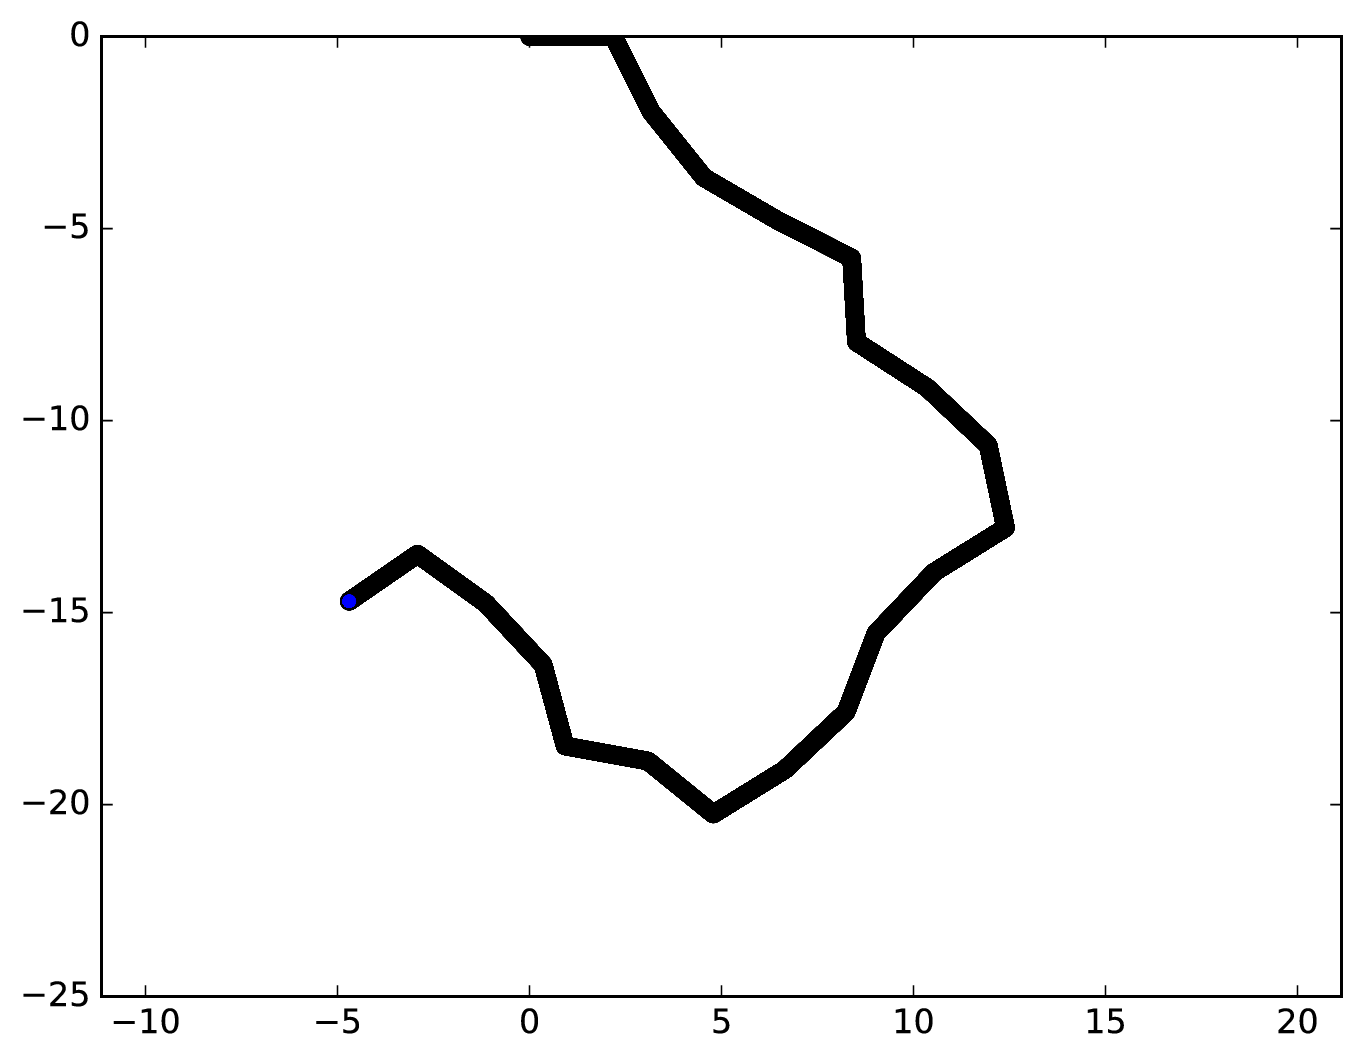
\includegraphics[width=\textwidth]{figures/ch3/synTraj_219_75_1}
			\caption[$A = 75$, $F=1$]{$A = 75$, $F=1$}
			\label{fig:synTraj_219_75_1}
		\end{subfigure}
		~
		\begin{subfigure}[t]{\subImgWmo}
			\centering
			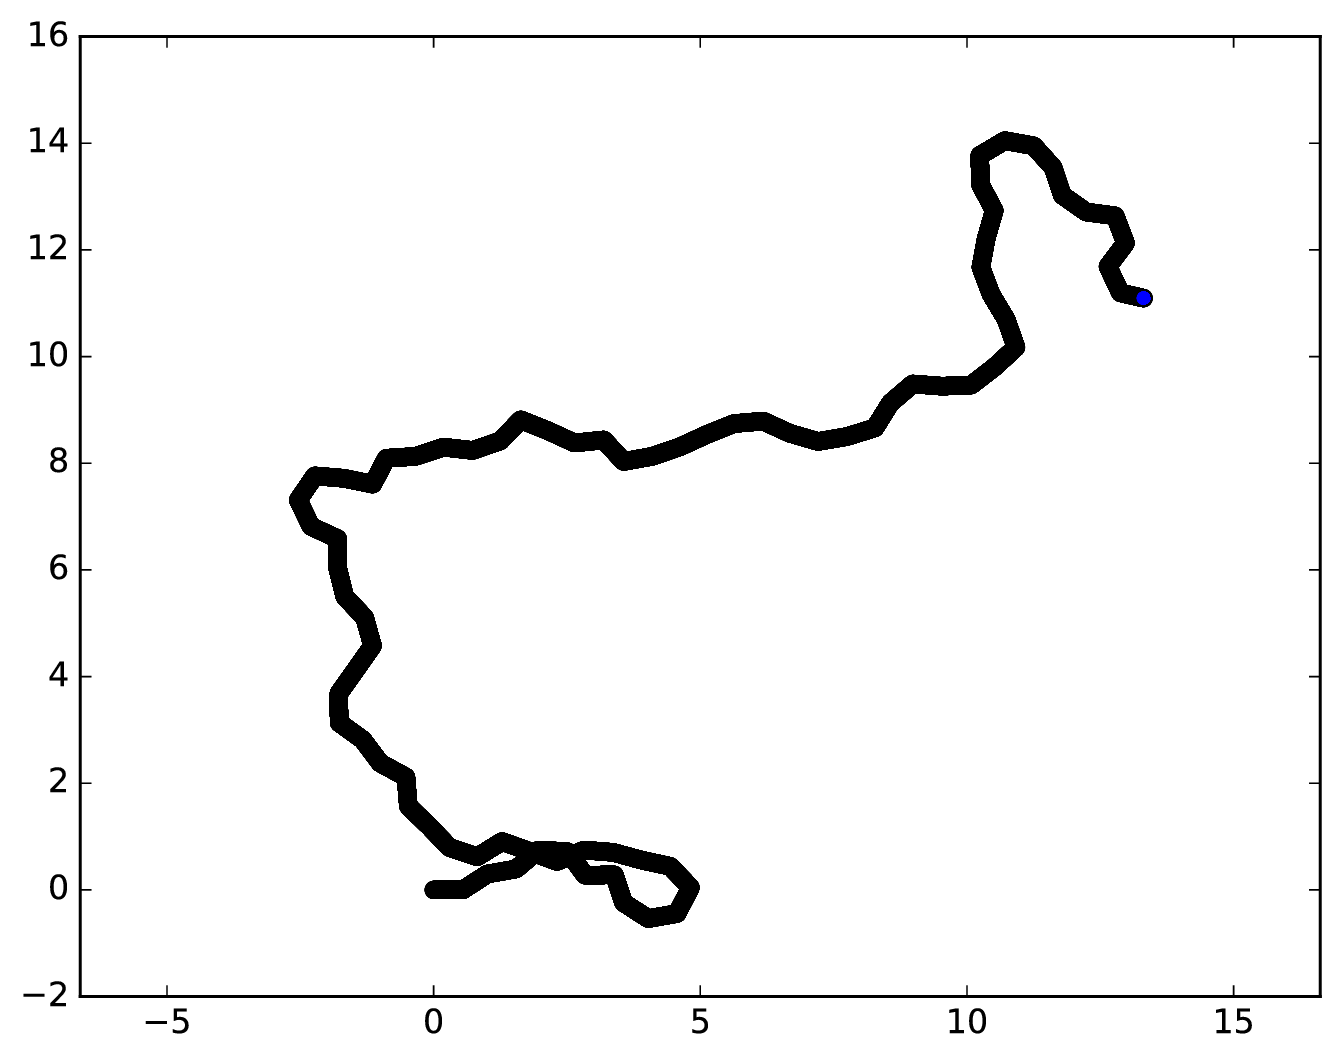
\includegraphics[width=\textwidth]{figures/ch3/synTraj_219_75_4}
			\caption[$A = 75$, $F=4$]{$A = 75$, $F=4$}
			\label{fig:synTraj_219_75_4}
		\end{subfigure}
		~
		\begin{subfigure}[t]{\subImgWmo}
			\centering
			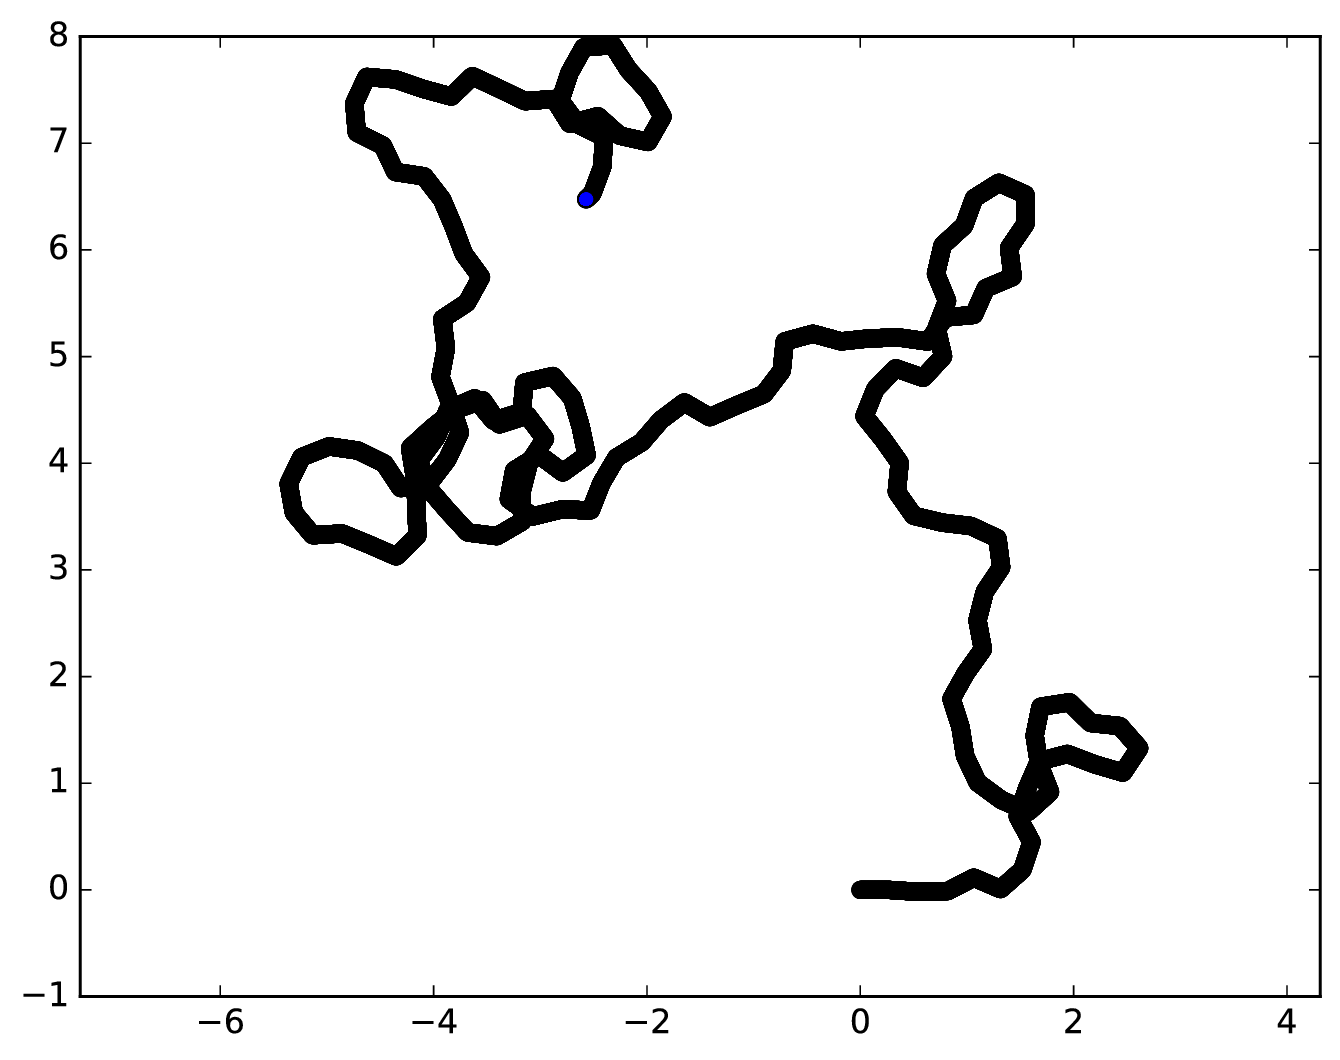
\includegraphics[width=\textwidth]{figures/ch3/synTraj_219_75_8}
			\caption[$A = 75$, $F=8$]{$A = 75$, $F=8$}
			\label{fig:synTraj_219_75_8}
		\end{subfigure}
		~
		\begin{subfigure}[t]{\subImgWmo}
			\centering
			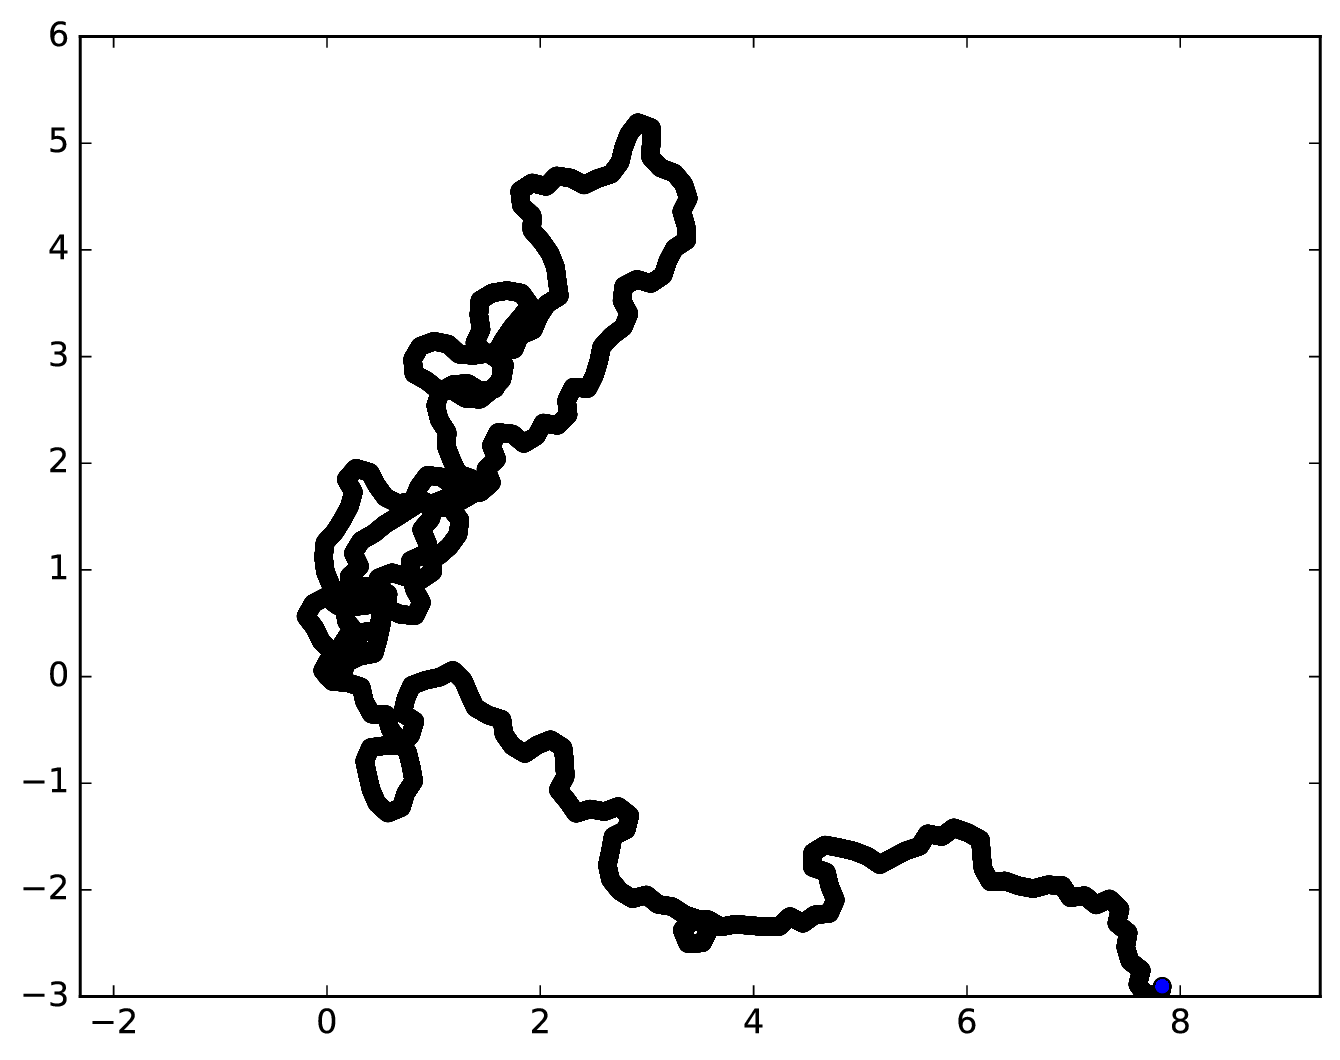
\includegraphics[width=\textwidth]{figures/ch3/synTraj_219_75_16}
			\caption[$A = 75$, $F=16$]{$A = 75$, $F=16$}
			\label{fig:synTraj_219_75_16}
		\end{subfigure}
		~
		\begin{subfigure}[t]{\subImgWmo}
			\centering
			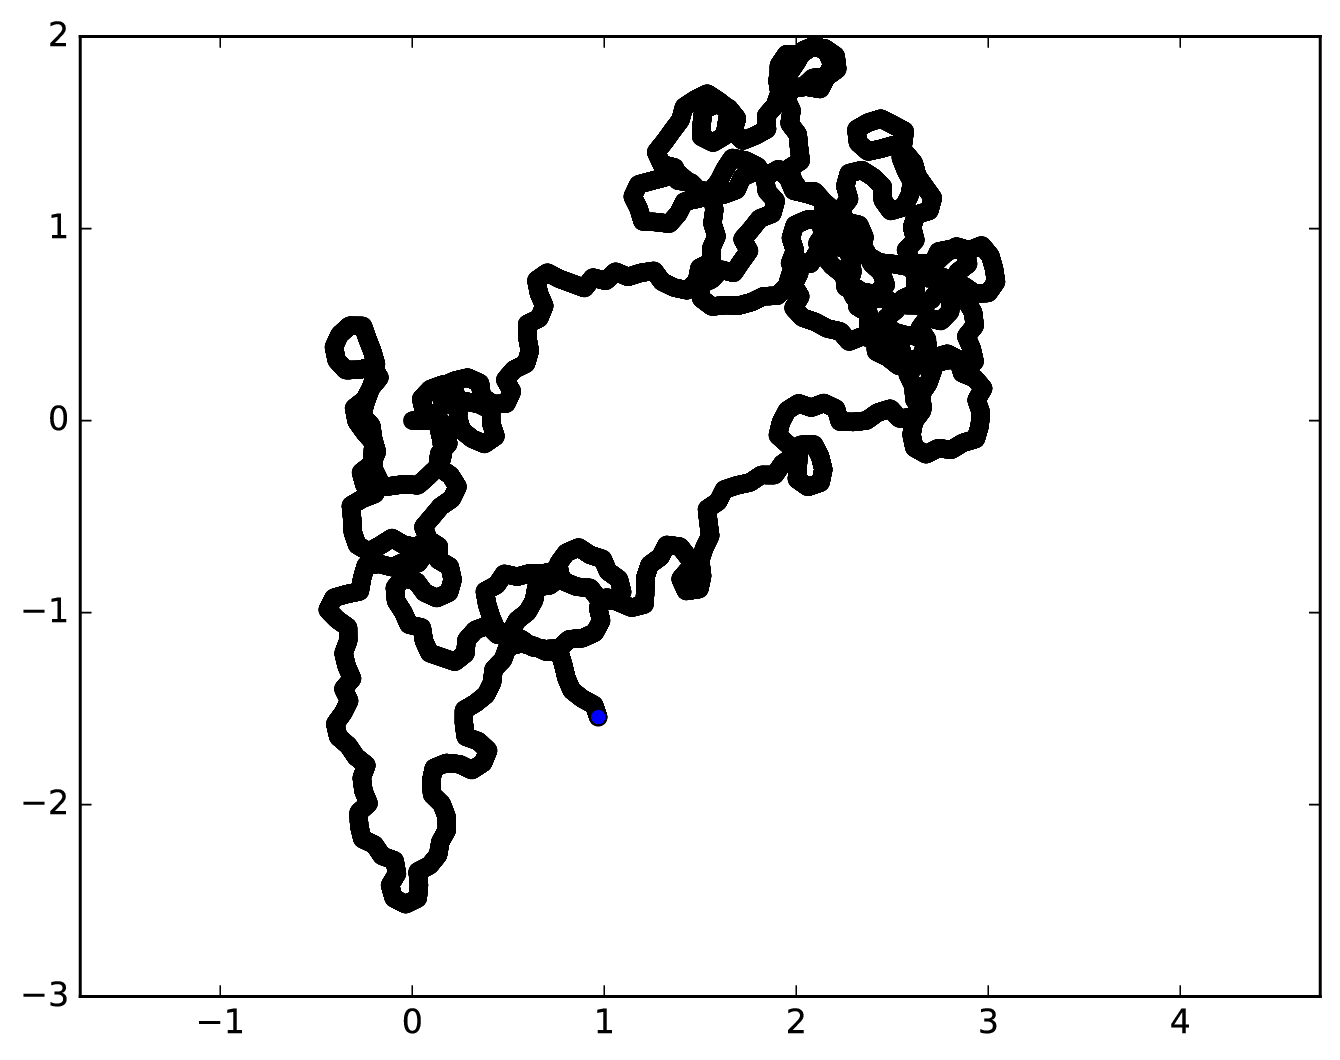
\includegraphics[width=\textwidth]{figures/ch3/synTraj_219_75_32}
			\caption[$A = 75$, $F=32$]{$A = 75$, $F=32$}
			\label{fig:synTraj_219_75_32}
		\end{subfigure}
		~
		\begin{subfigure}[t]{\subImgWmo}
			\centering
			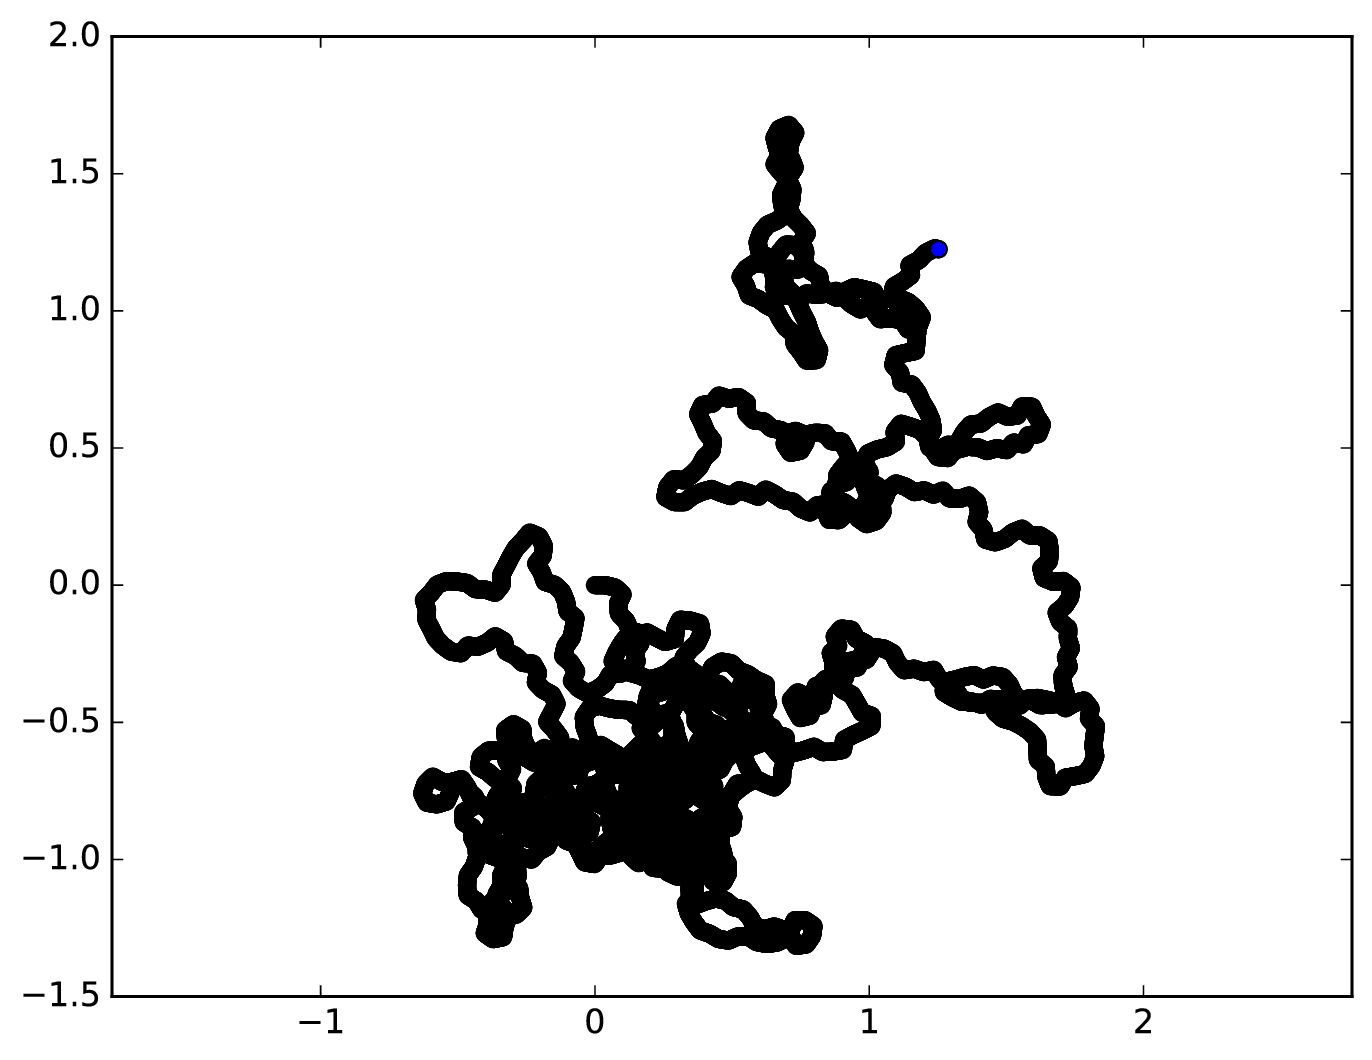
\includegraphics[width=\textwidth]{figures/ch3/synTraj_219_75_60}
			\caption[$A = 75$, $F=60$]{$A = 75$, $F=60$}
			\label{fig:synTraj_219_75_60}
		\end{subfigure}
		~
		\begin{subfigure}[t]{\subImgWmo}
			\centering
			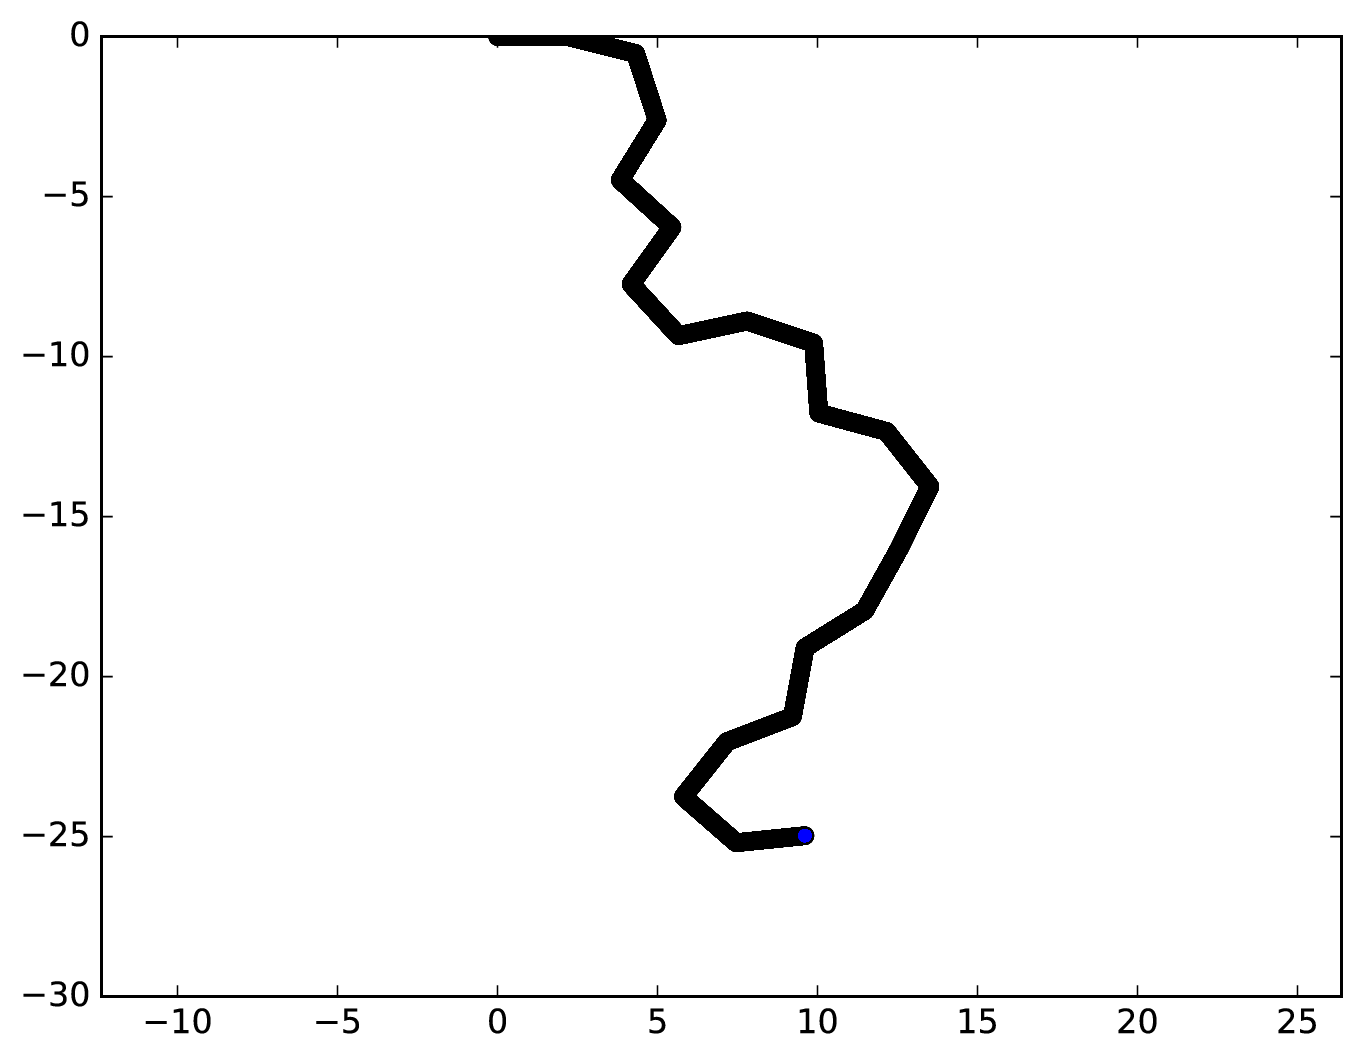
\includegraphics[width=\textwidth]{figures/ch3/synTraj_219_90_1}
			\caption[$A = 90$, $F=1$]{$A = 90$, $F=1$}
			\label{fig:synTraj_219_90_1}
		\end{subfigure}
		~
		\begin{subfigure}[t]{\subImgWmo}
			\centering
			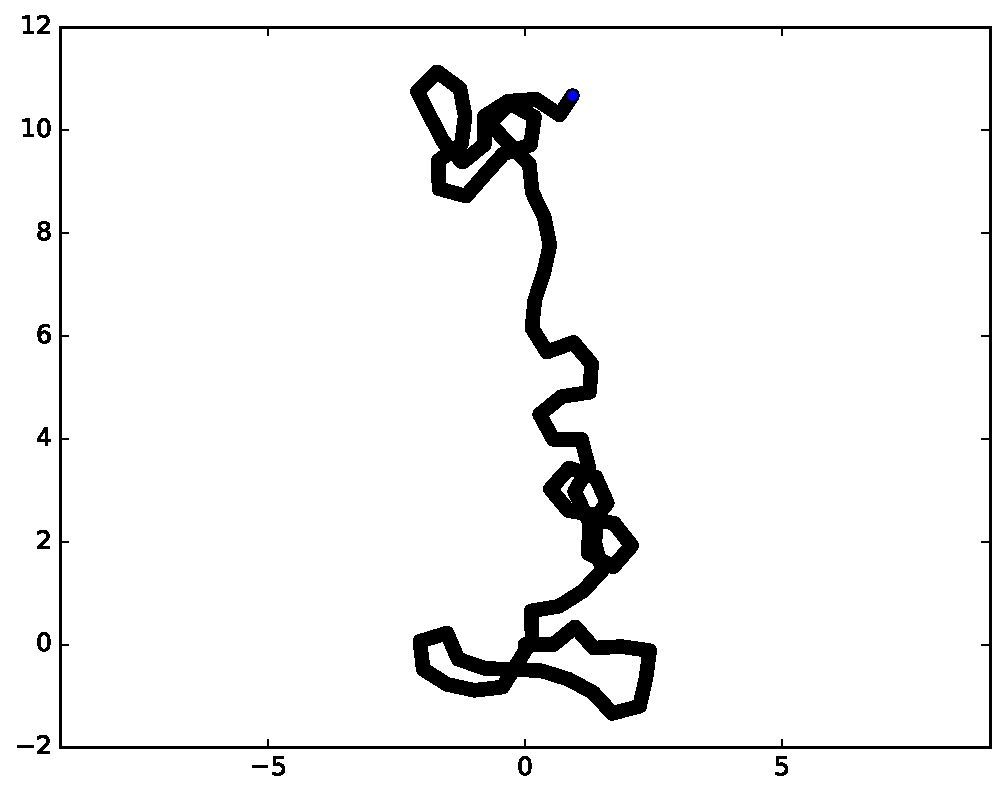
\includegraphics[width=\textwidth]{figures/ch3/synTraj_219_90_4}
			\caption[$A = 90$, $F=4$]{$A = 90$, $F=4$}
			\label{fig:synTraj_219_90_4}
		\end{subfigure}
		~
		\begin{subfigure}[t]{\subImgWmo}
			\centering
			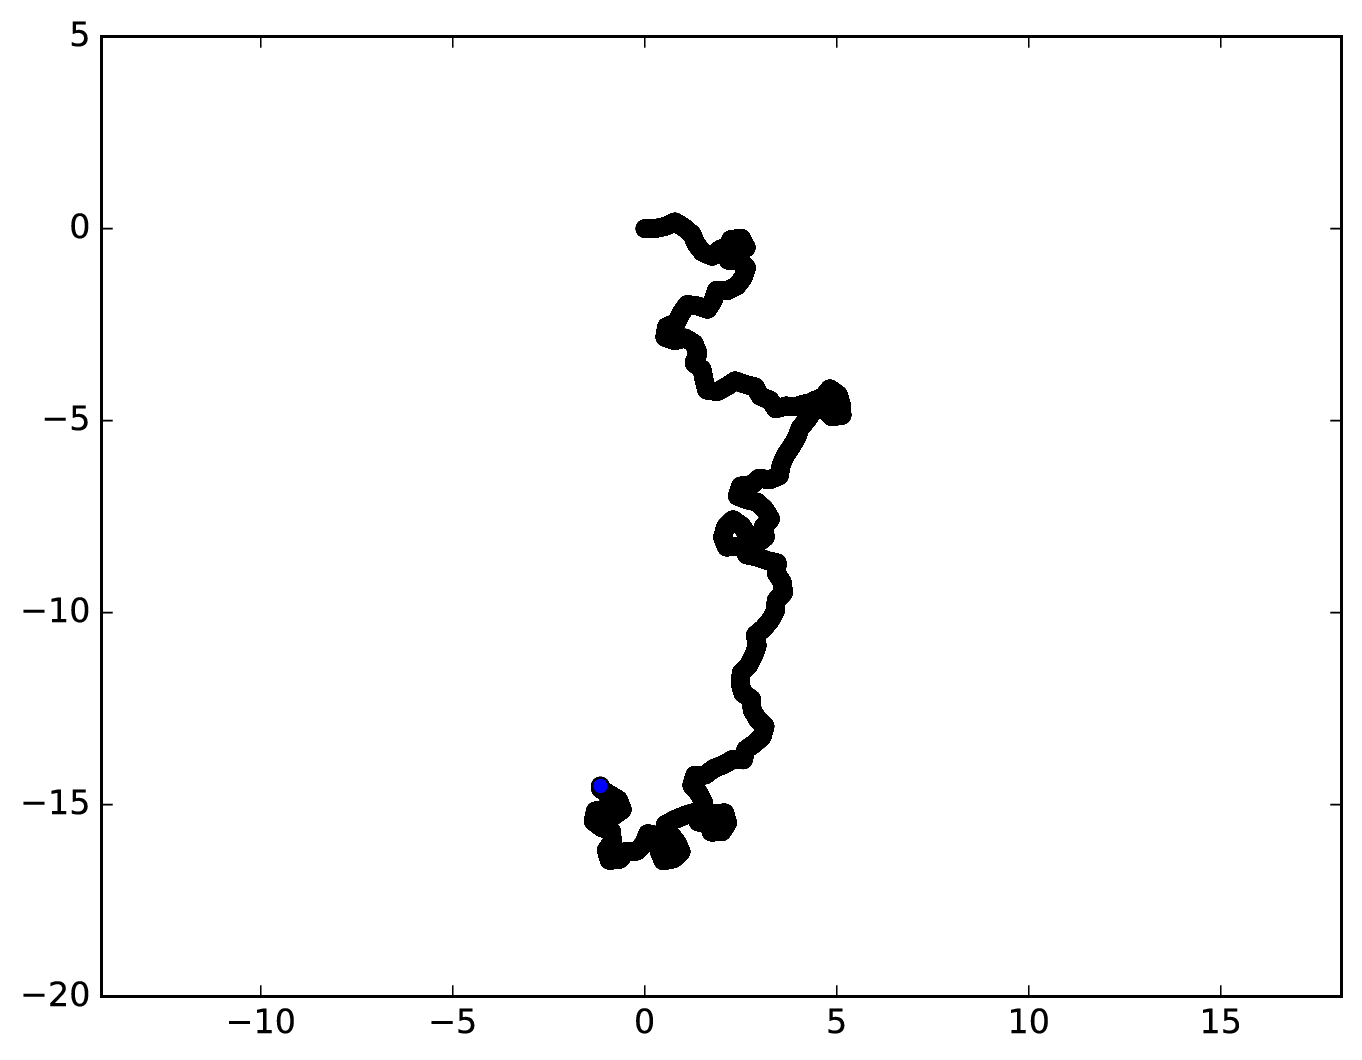
\includegraphics[width=\textwidth]{figures/ch3/synTraj_219_90_8}
			\caption[$A = 90$, $F=8$]{$A = 90$, $F=8$}
			\label{fig:synTraj_219_90_8}
		\end{subfigure}
		~
		\begin{subfigure}[t]{\subImgWmo}
			\centering
			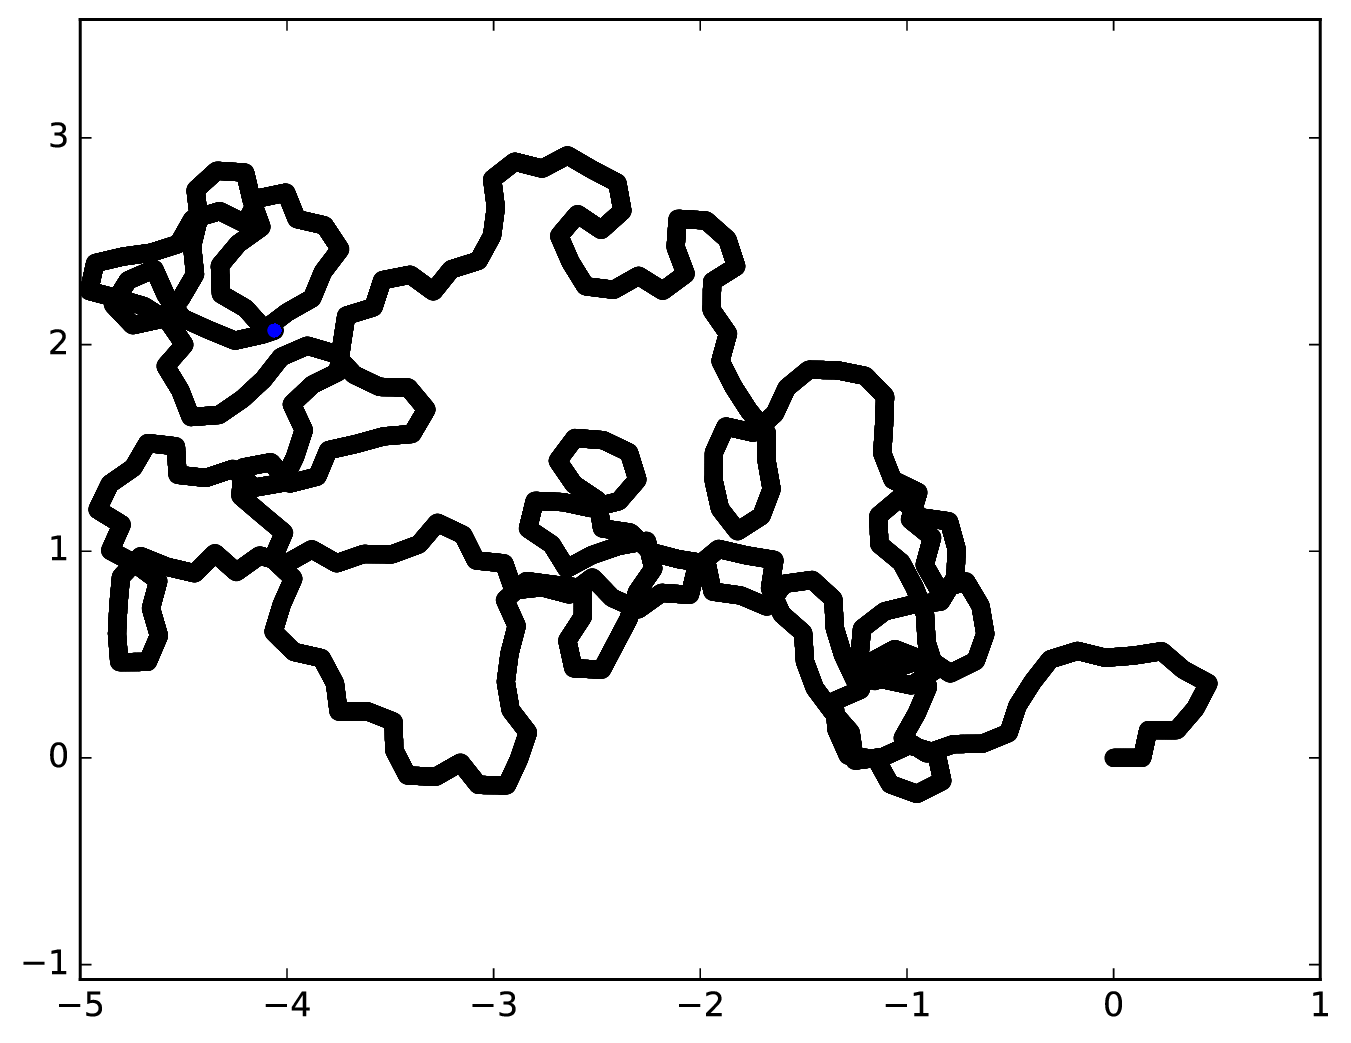
\includegraphics[width=\textwidth]{figures/ch3/synTraj_219_90_16}
			\caption[$A = 90$, $F=16$]{$A = 90$, $F=16$}
			\label{fig:synTraj_219_90_16}
		\end{subfigure}
		~
		\begin{subfigure}[t]{\subImgWmo}
			\centering
			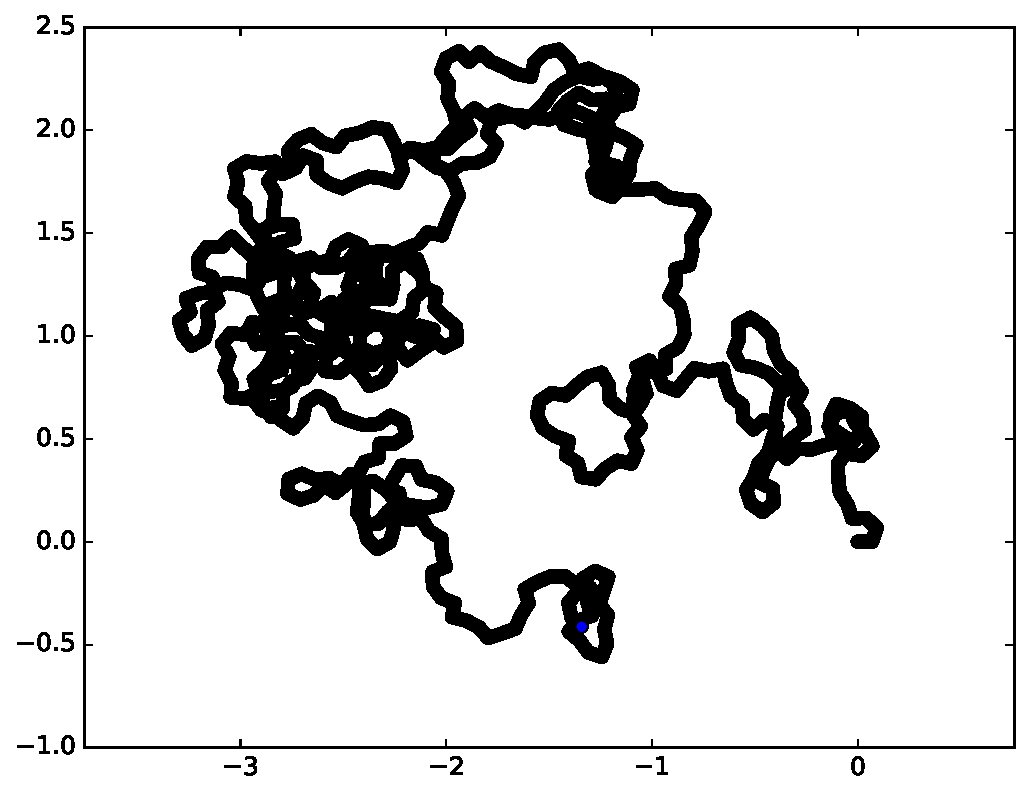
\includegraphics[width=\textwidth]{figures/ch3/synTraj_219_90_32}
			\caption[$A = 90$, $F=32$]{$A = 90$, $F=32$}
			\label{fig:synTraj_219_90_32}
		\end{subfigure}
		~
		\begin{subfigure}[t]{\subImgWmo}
			\centering
			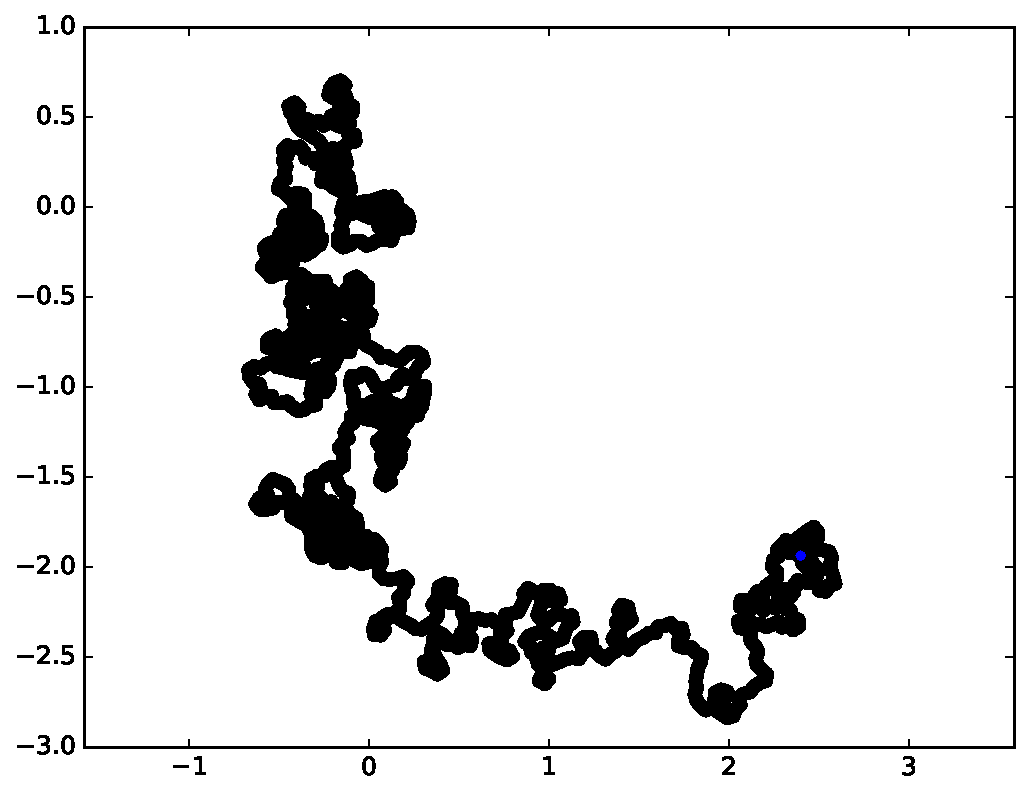
\includegraphics[width=\textwidth]{figures/ch3/synTraj_219_90_60}
			\caption[$A = 90$, $F=60$]{$A = 90$, $F=60$}
			\label{fig:synTraj_219_90_60}
		\end{subfigure}
		\caption[Mouvements générés par notre modèle -- III]{Exemples de trajectoires générées par notre modèle pour un objet de vitesse constante (2,19~cm/s).}
		\label{fig:motion7590}
	\end{figure}
	
	Nous proposons ici un examen détaillé de quelques trajectoires. Avant tout autre propos, que le lecteur nous permette d'attirer son attention sur le fait que les trajectoires illustrées sur les figures~\ref{fig:motion1530}, \ref{fig:motion4560}, \ref{fig:motion7590}, \ref{fig:motion105120}, \ref{fig:motion135150} et \ref{fig:motion165180} sont représentées à des échelles différentes. En effet, la trajectoire de la figure~\ref{fig:synTraj_219_15_1} parcourt plus de 40~cm à l'horizontale, tandis que celle de la figure~\ref{fig:synTraj_219_180_60} est contenue dans un rectangle d'environ 1,2~cm de hauteur sur 1~cm de largeur.
	
	Il est donc inévitable de représenter ces trajectoires à des échelles adaptées si l'on souhaite qu'elles soient lisibles, mais il convient de faire attention à l'échelle et de garder à l'esprit que les trajectoires les plus irrégulières sont généralement représentées à une échelle bien plus fine.
	
	\subsubsection{Effet des vitesses}
	Modifier la vitesse d'un objet ne change pas la \og nature \fg{} du mouvement ni, au sens strict, son entropie. En effet, pour des valeurs de $A$ et $F$ données et une position donnée à l'instant $t$, le nombre d'états possible à l'instant $t+1$ ne dépend pas de la vitesse. On observe cependant qu'à mesure que la vitesse croît, une \og dilatation \fg{} des trajectoires s'opère, comme l'illustre la figure~\ref{fig:spEffect}, comparant diverses trajectoires générées avec des vitesses différentes mais des valeurs de $A$ et $F$ constantes.
	
	Il convient toutefois d'être prudent en interprétant cette donnée. En effet, si le nombre d'états possibles est objectivement le même, ces états ne sont pas nécessairement équivalents entre eux du point de vue subjectif d'un utilisateur tentant de sélectionner l'objet. En effet, si l'on suppose par exemple que l'objet en question est une sphère de 1~cm de diamètre, si elle se déplace à 0,5~cm/s, au bout d'une seconde une partie de l'objet sera toujours dans l'espace qu'il occupait à la seconde précédente ; pour une vitesse de 4~cm/s, ce n'est pas nécessairement le cas. La figure~\ref{fig:spTraj_0_5_120_2} montre qu'à basse vitesse (et à partir d'un certain niveau de pseudo-entropie) la cible évolue dans un espace très restreint ; inversement, quand la vitesse est élevée, comme sur la figure~\ref{fig:spTraj_4_0_120_2}, cette zone peut devenir très grande.
	
	Plus généralement, une cible d'une entropie donnée pourra s'éloigner d'autant plus rapidement du curseur de l'utilisateur que sa vitesse est élevée, et nous savons depuis les travaux de Fitts que la distance au curseur est déterminante pour la difficulté de sélection. Remarquons simplement ici, et avant d'analyser des données quantitatives précises, que si la vitesse d'un objet ne modifie pas son entropie, ces deux valeurs doivent être examinées conjointement pour (espérer) caractériser correctement la difficulté de sélection.	

	\begin{figure}[htb]
		\centering
		\begin{subfigure}[t]{\subImgWarea}
			\centering
			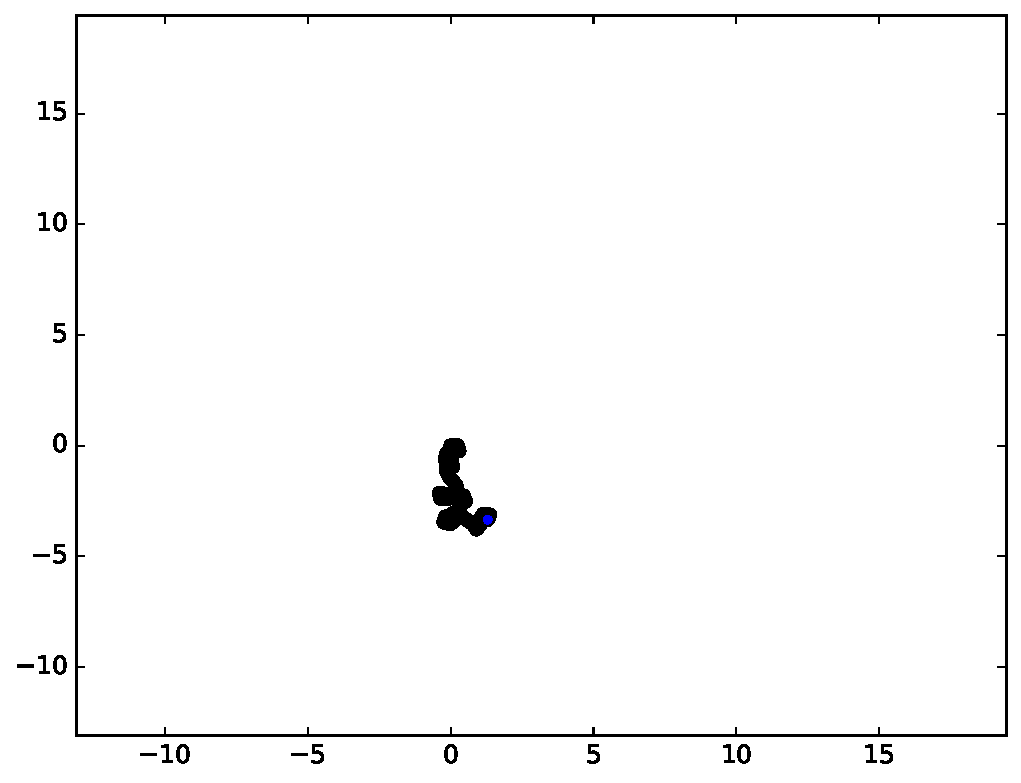
\includegraphics[width=\textwidth]{figures/ch3/spTraj_0_5_120_2}
			\caption[$S = 0,5$]{$S = 0,5$~cm/s.}
			\label{fig:spTraj_0_5_120_2}
		\end{subfigure}
		~
		\begin{subfigure}[t]{\subImgWarea}
			\centering
			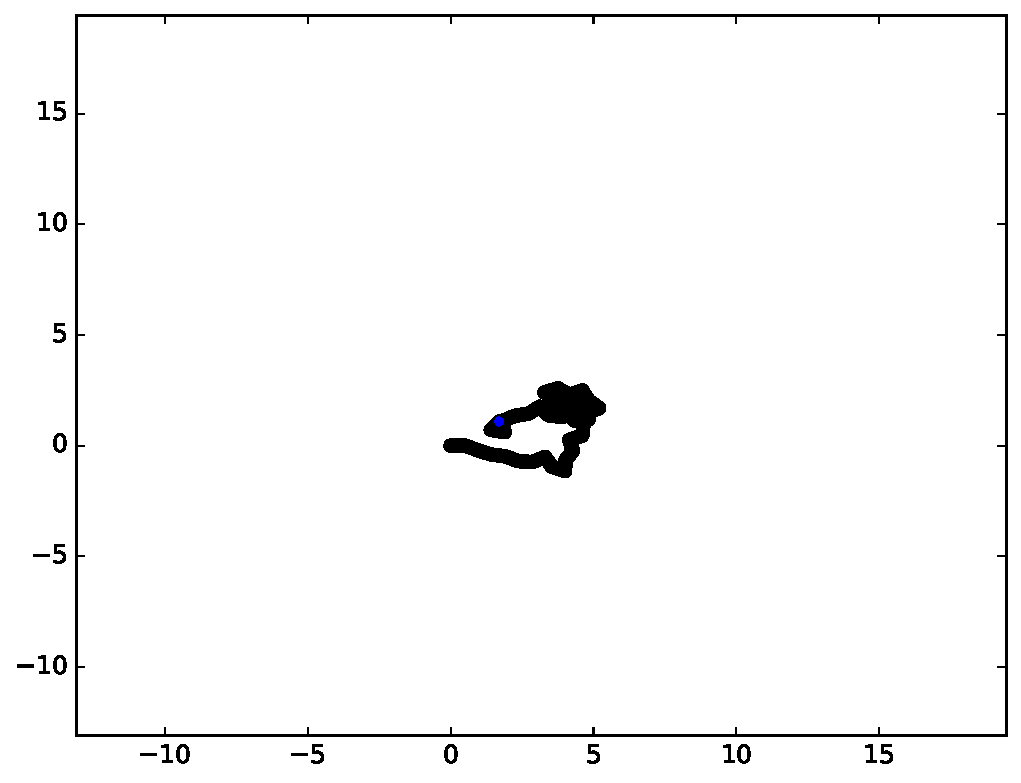
\includegraphics[width=\textwidth]{figures/ch3/spTraj_1_0_120_2}
			\caption[$S = 1$]{$S = 1$~cm/s.}
			\label{fig:spTraj_1_0_120_2}
		\end{subfigure}
		~
		\begin{subfigure}[t]{\subImgWarea}
			\centering
			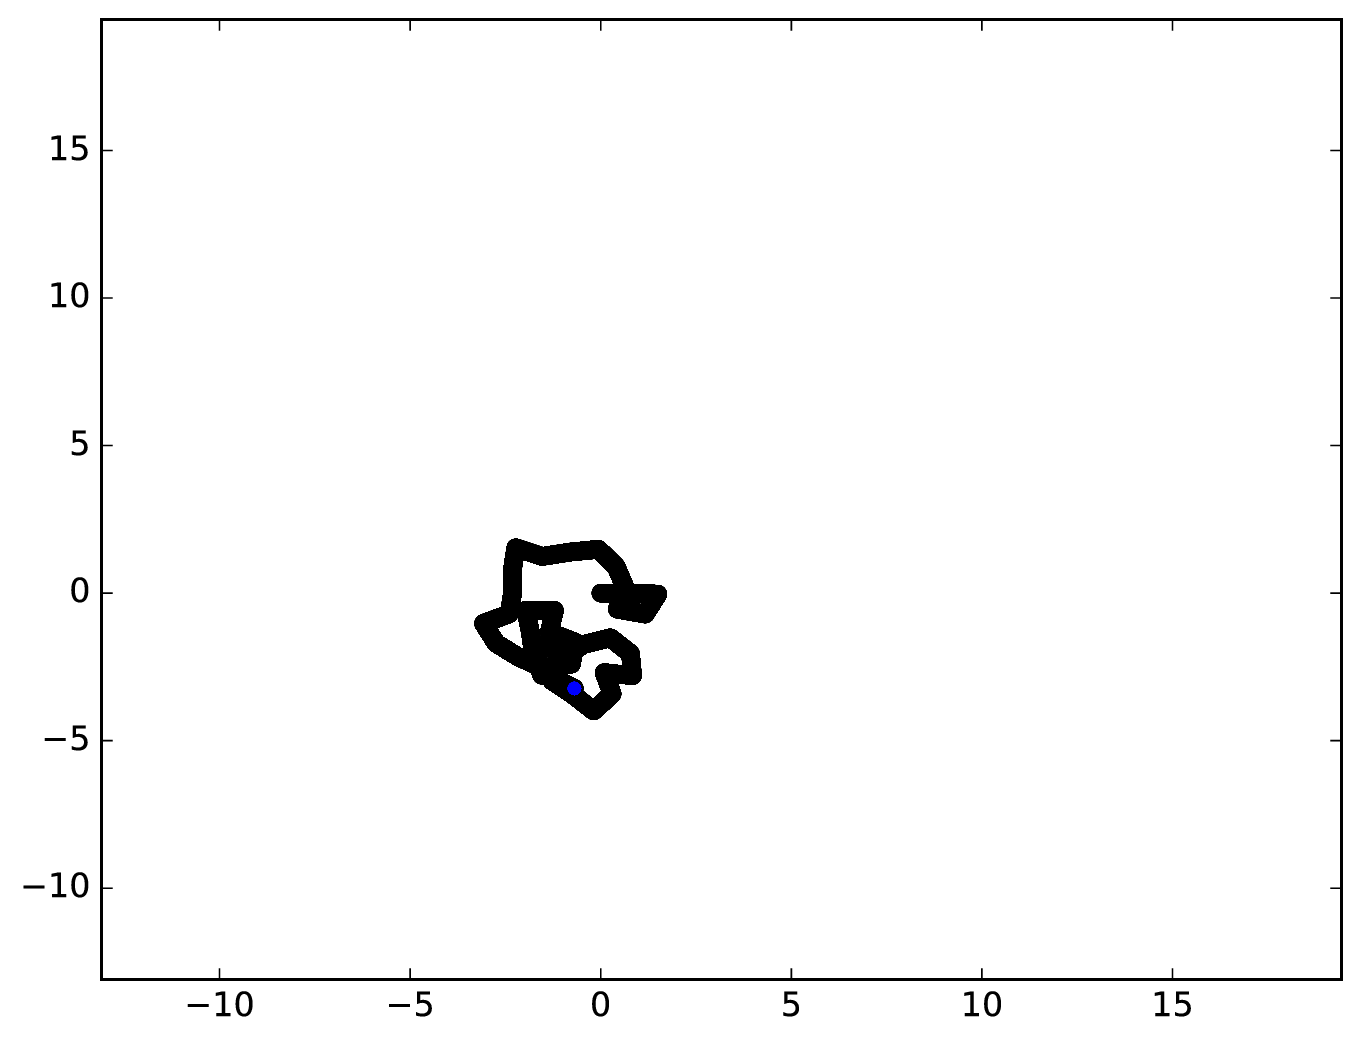
\includegraphics[width=\textwidth]{figures/ch3/spTraj_1_5_120_2}
			\caption[$S = 1,5$]{$S = 1,5$~cm/s.}
			\label{fig:spTraj_1_5_120_2}
		\end{subfigure}
		~
		\begin{subfigure}[t]{\subImgWarea}
			\centering
			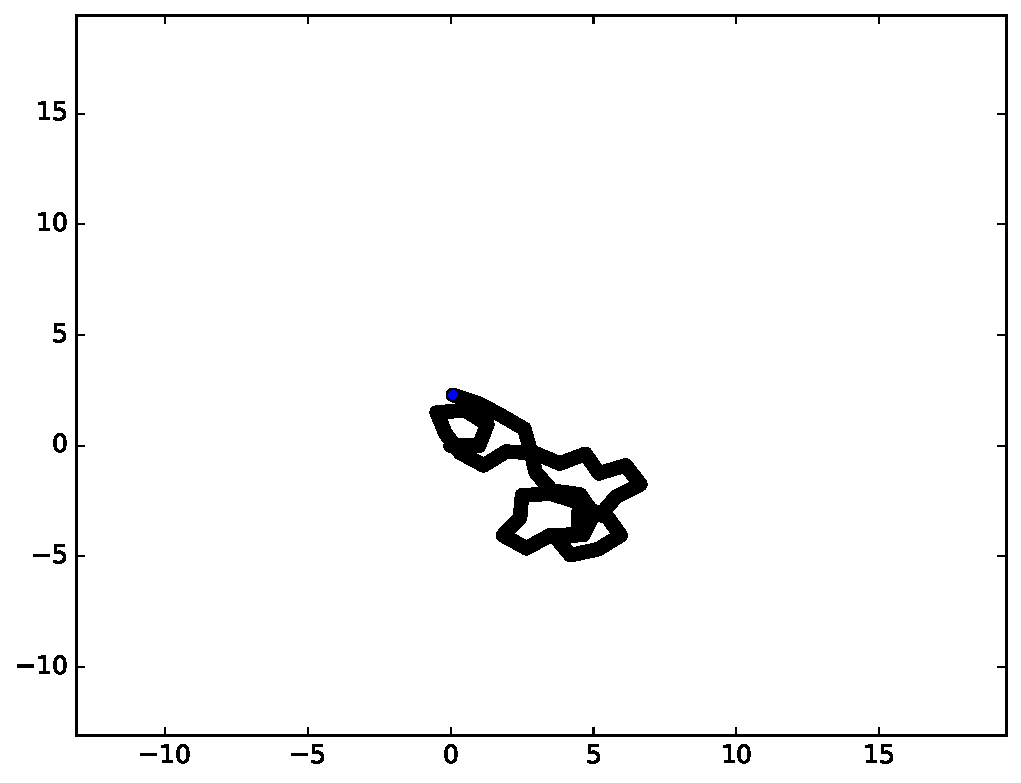
\includegraphics[width=\textwidth]{figures/ch3/spTraj_2_0_120_2}
			\caption[$S = 2,0$]{$S = 2,0$~cm/s.}
			\label{fig:spTraj_2_0_120_2}
		\end{subfigure}
		~
		\begin{subfigure}[t]{\subImgWarea}
			\centering
			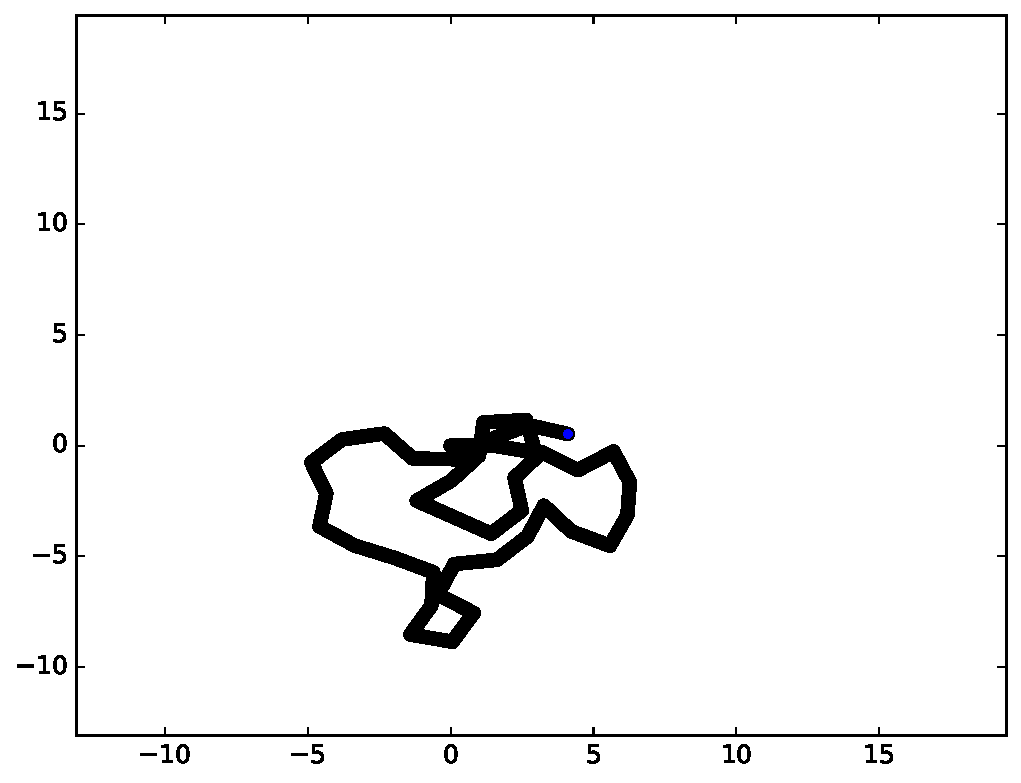
\includegraphics[width=\textwidth]{figures/ch3/spTraj_3_0_120_2}
			\caption[$S = 3,0$]{$S = 3,0$~cm/s.}
			\label{fig:spTraj_3_0_120_2}
		\end{subfigure}
		~
		\begin{subfigure}[t]{\subImgWarea}
			\centering
			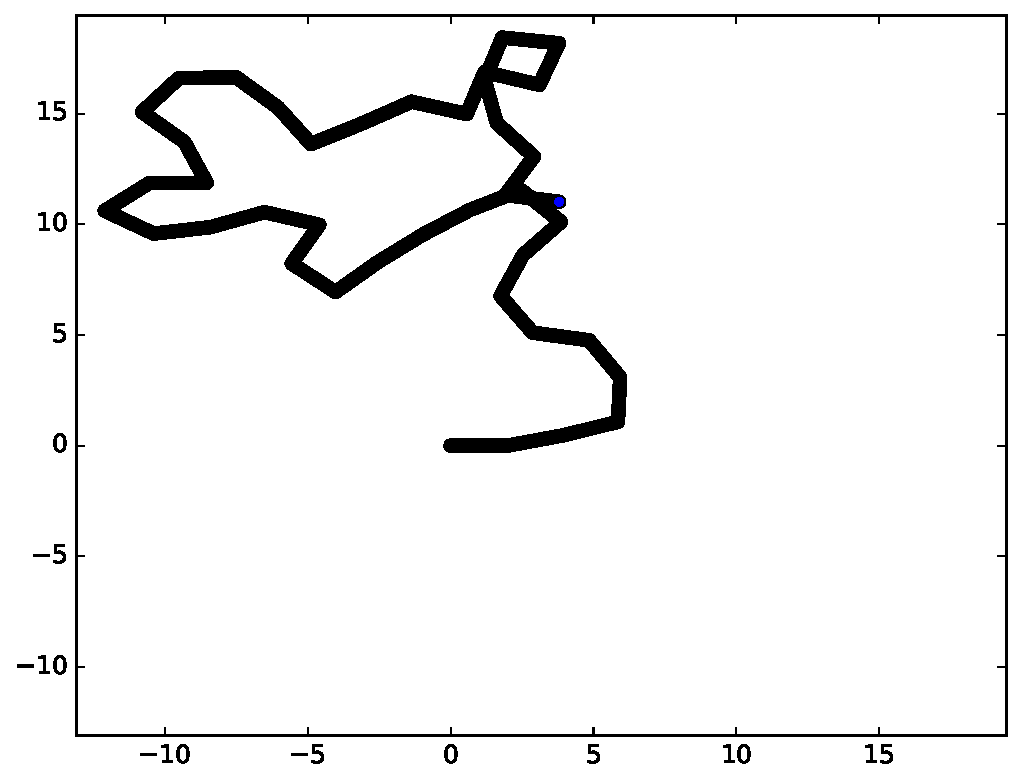
\includegraphics[width=\textwidth]{figures/ch3/spTraj_4_0_120_2}
			\caption[$S = 4,0$]{$S = 4,0$~cm/s.}
			\label{fig:spTraj_4_0_120_2}
		\end{subfigure}
		\caption[Effet des vitesses]{Trajectoires générées avec $A = 120\degree$ et $F = 2$~Hz, et des vitesses variables, de 0,5~cm/s à 4,0~cm/s. Notez que pour mieux observer le phénomène de \og dilatation \fg{} des trajectoires, et contrairement à la plupart des figures de ce type incluses dans ce manuscrit, l'échelle est constante pour toutes les sous-figures.}
		\label{fig:spEffect}
	\end{figure}
	
	\subsubsection{Effet des angles}
	Lorque $A$ est faible, comme sur la figure~\ref{fig:motion1530}, le mouvement est relativement lisse et régulier, avec des courbes infréquentes et douces, sauf quand la valeur de $F$ augmente beaucoup ; et encore les trajectoires apparaissent-elles relativement \og dénouées \fg{}, à l'exception de celle de la figure~\ref{fig:synTraj_219_30_60} dont les valeurs de $A$ et $F$ commencent à être élevées, avec 30\textdegree{} et 60~Hz respectivement.
	
	À mesure que $A$ augmente, comme le montrera un examen successif des figures~\ref{fig:motion1530}, \ref{fig:motion4560}, \ref{fig:motion7590}, \ref{fig:motion105120}, \ref{fig:motion135150} et \ref{fig:motion165180}, les trajectoires sont de plus en plus irrégulières et \og nouées \fg{}.
	
	\subsubsection{Effet des fréquences}
	Un examen de n'importe quel bloc de six trajectoires pour une valeur de $A$ donnée montrera que plus $F$ est grand, plus les trajectoires sont irrégulières. Cet effet est très net et tout aussi visible quand $A$ est petit (comme sur la figure~\ref{fig:motion1530}) que quand il est grand (comme sur la figure~\ref{fig:motion165180}).
	
	Toutefois, quand $A$ est très grand, même avec une petite valeur de $F$, la trajectoire présente d'importantes irrégularités, comme sur la figure~\ref{fig:synTraj_219_180_1}. Notez cependant d'une part que ce n'est vrai que parce que nous observons la trajectoire sur une fenêtre temporelle relativement longue (20 secondes) et d'autre part que nous aurions pu choisir une valeur de $F$ bien plus faible, comme 0,1~Hz, par exemple, voire moins. Si $F$ était strictement inférieure à 0,05~Hz, sur une fenêtre de 20 secondes, la trajectoire serait rectiligne.
	
	\begin{figure}[htb]
		\begin{subfigure}[t]{\subImgWmo}
			\centering
			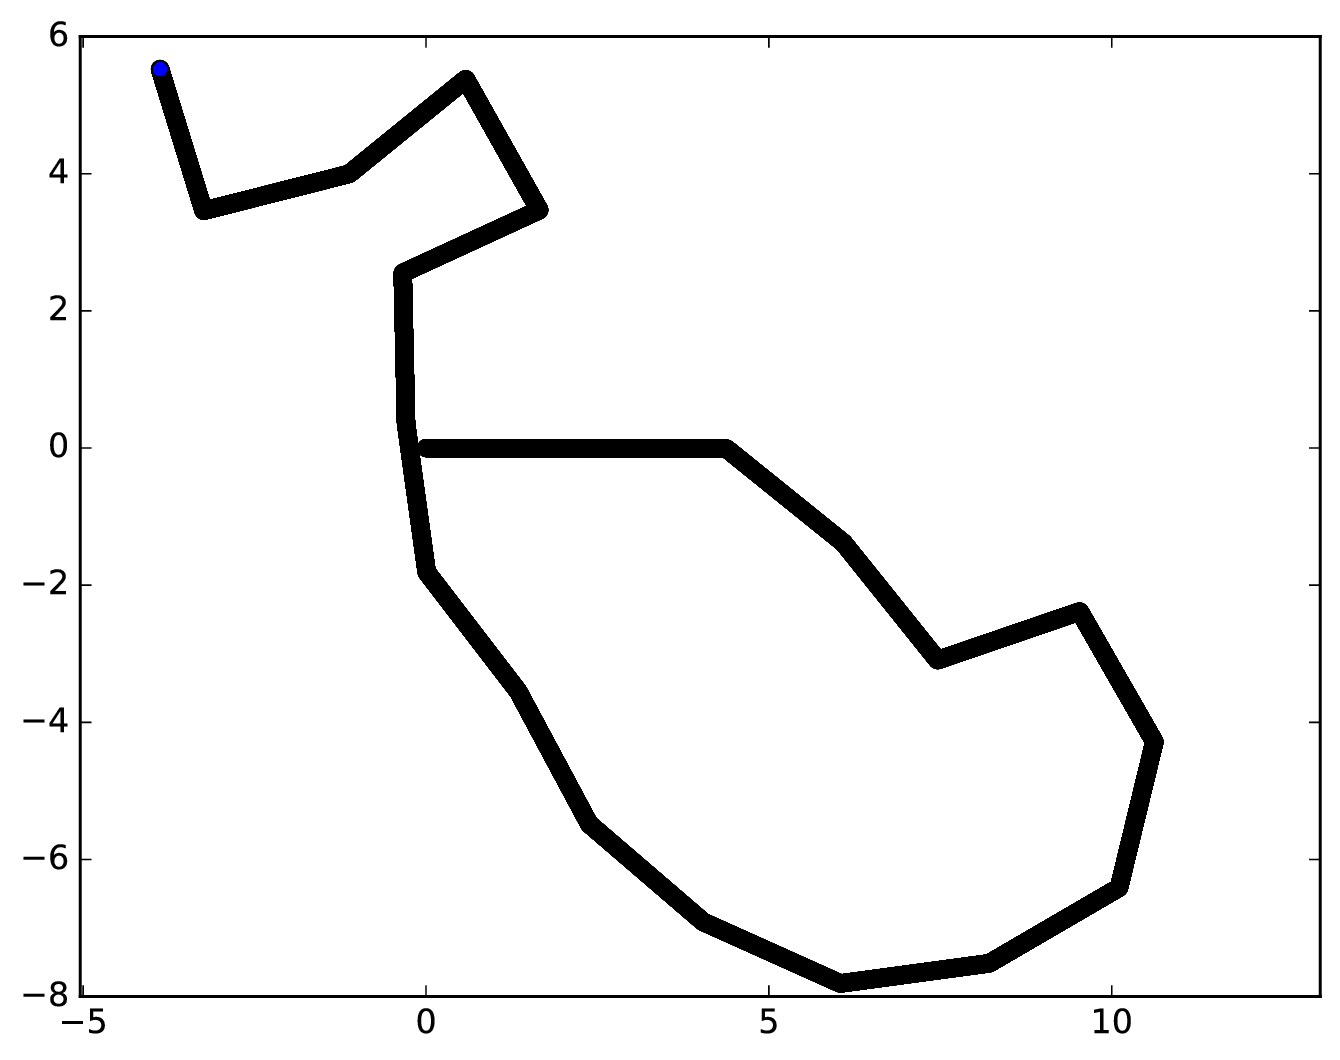
\includegraphics[width=\textwidth]{figures/ch3/synTraj_219_105_1}
			\caption[$A = 105$, $F=1$]{$A = 105$, $F=1$}
			\label{fig:synTraj_219_105_1}
		\end{subfigure}
		~
		\begin{subfigure}[t]{\subImgWmo}
			\centering
			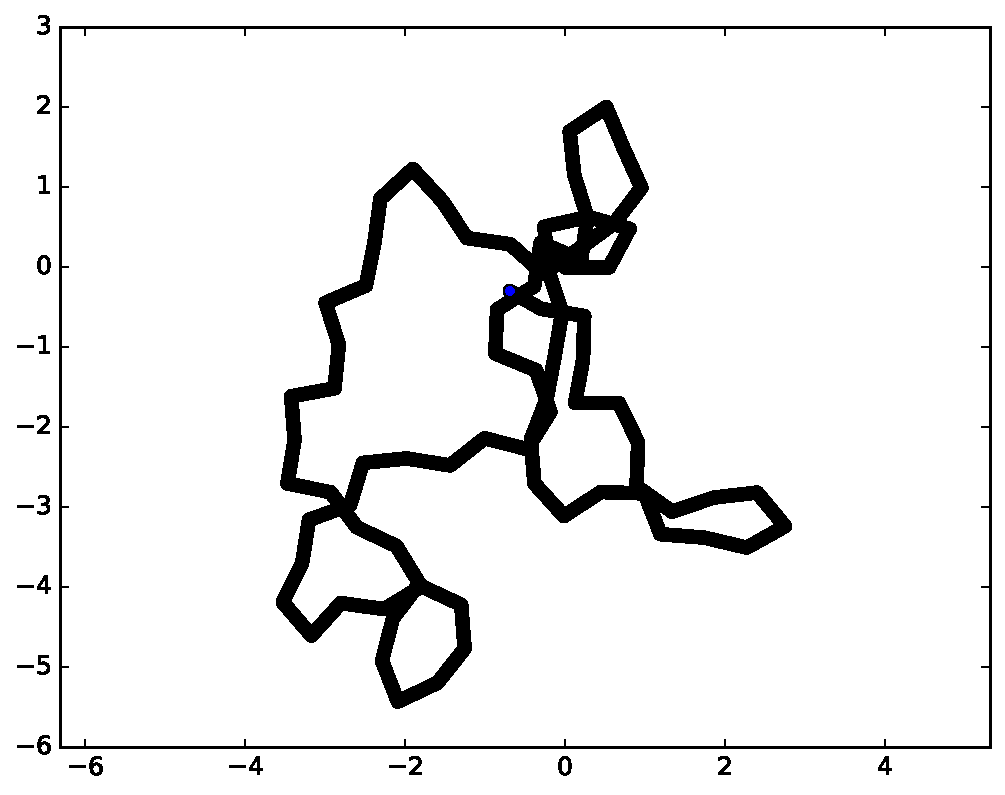
\includegraphics[width=\textwidth]{figures/ch3/synTraj_219_105_4}
			\caption[$A = 105$, $F=4$]{$A = 105$, $F=4$}
			\label{fig:synTraj_219_105_4}
		\end{subfigure}
		~
		\begin{subfigure}[t]{\subImgWmo}
			\centering
			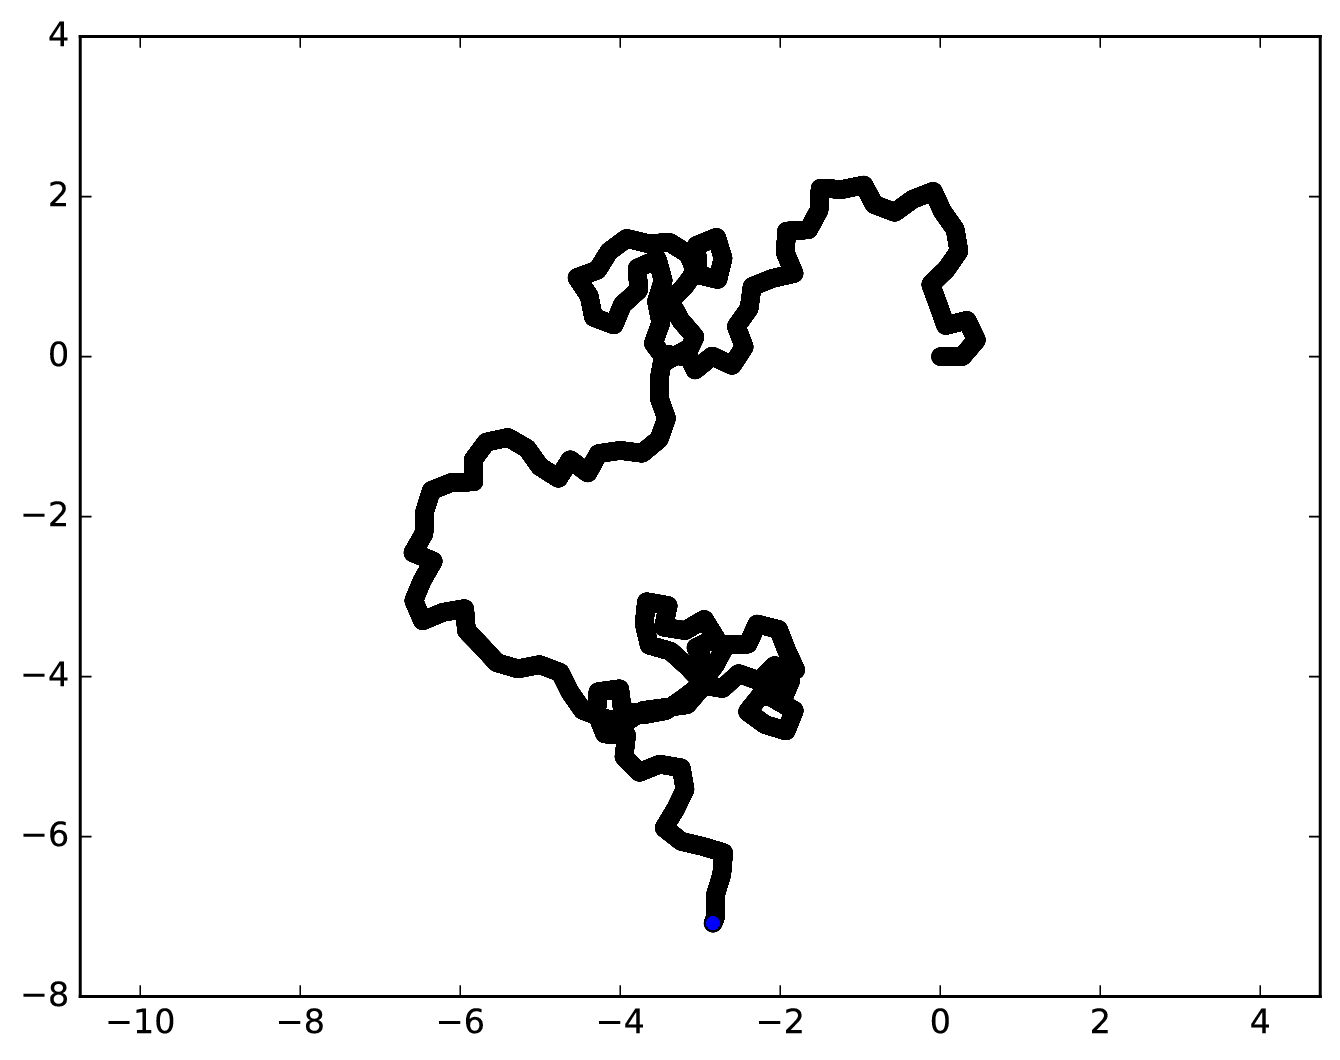
\includegraphics[width=\textwidth]{figures/ch3/synTraj_219_105_8}
			\caption[$A = 105$, $F=8$]{$A = 105$, $F=8$}
			\label{fig:synTraj_219_105_8}
		\end{subfigure}
		~
		\begin{subfigure}[t]{\subImgWmo}
			\centering
			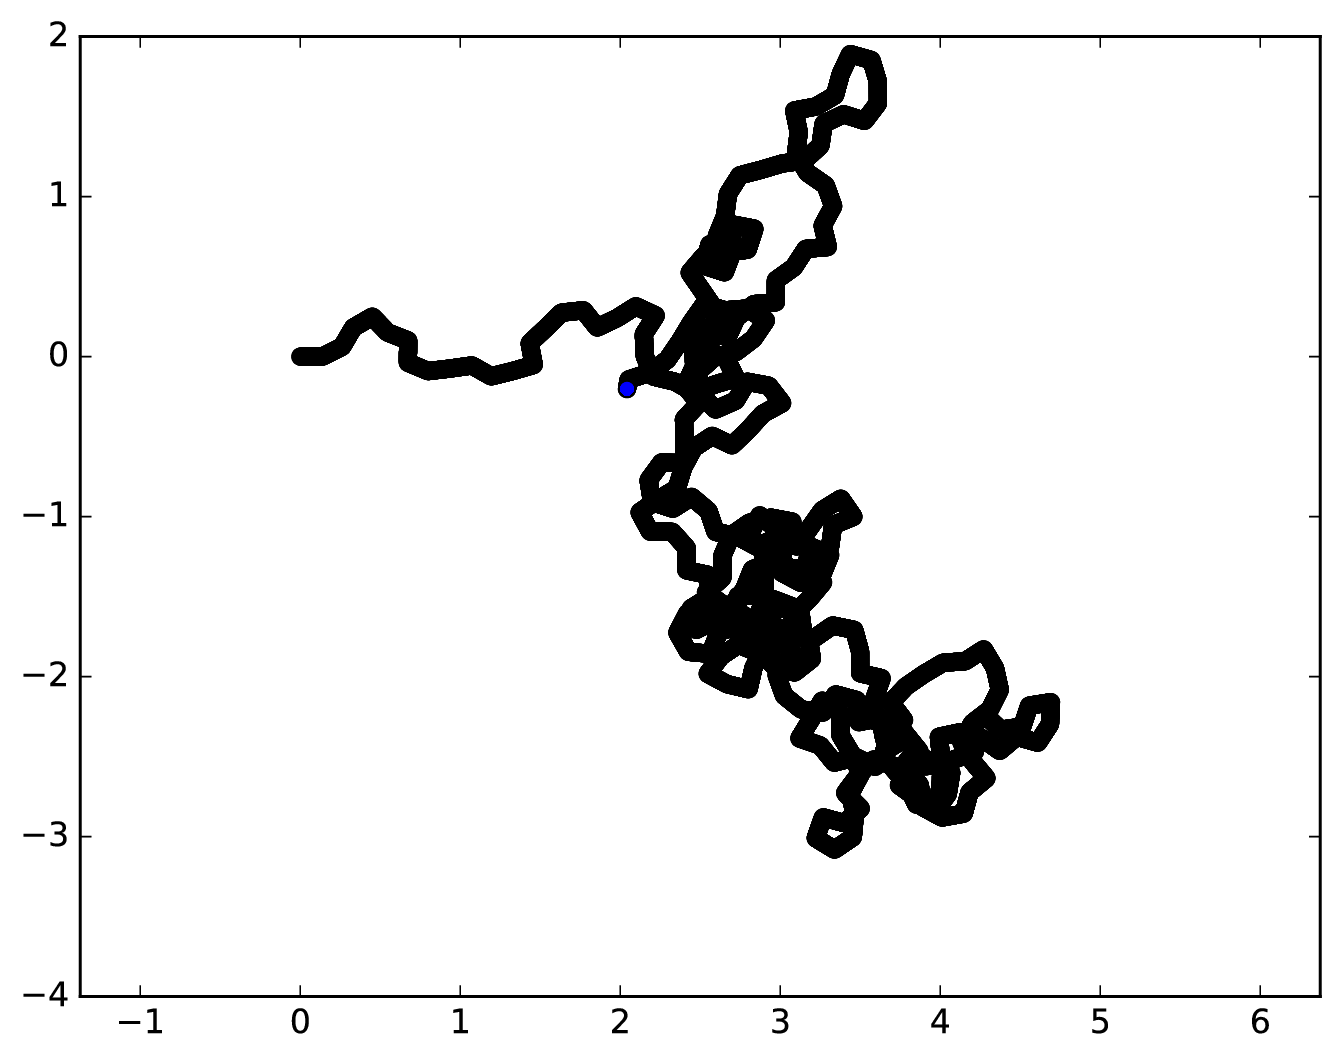
\includegraphics[width=\textwidth]{figures/ch3/synTraj_219_105_16}
			\caption[$A = 105$, $F=16$]{$A = 105$, $F=16$}
			\label{fig:synTraj_219_105_16}
		\end{subfigure}
		~
		\begin{subfigure}[t]{\subImgWmo}
			\centering
			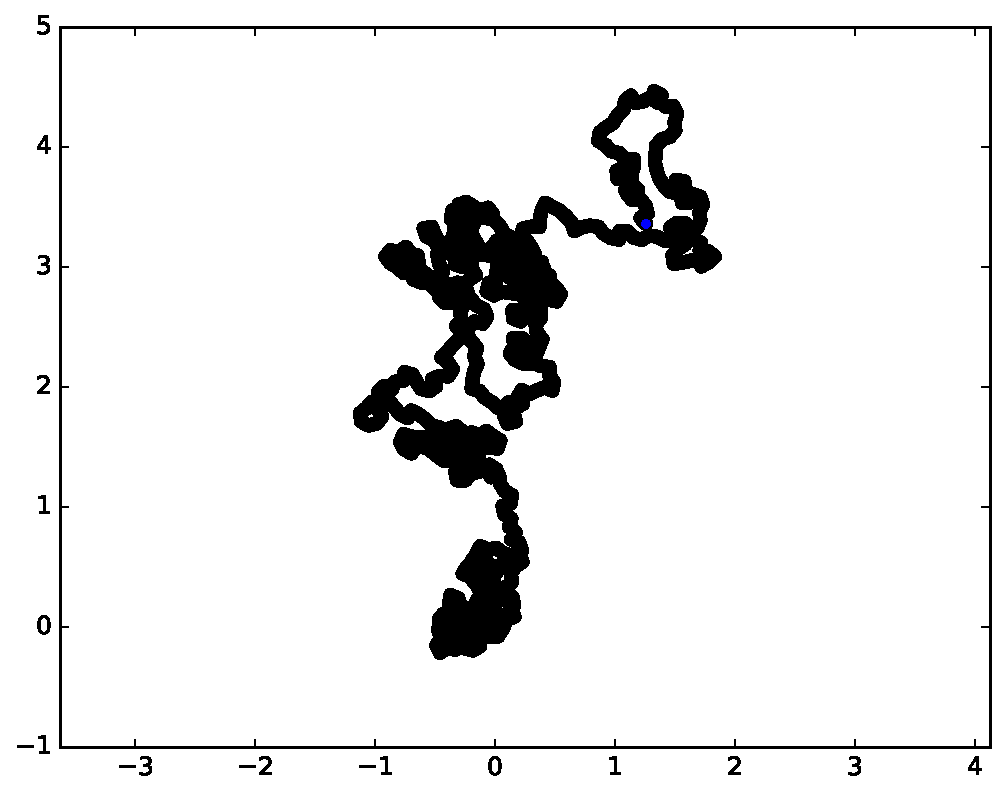
\includegraphics[width=\textwidth]{figures/ch3/synTraj_219_105_32}
			\caption[$A = 105$, $F=32$]{$A = 105$, $F=32$}
			\label{fig:synTraj_219_105_32}
		\end{subfigure}
		~
		\begin{subfigure}[t]{\subImgWmo}
			\centering
			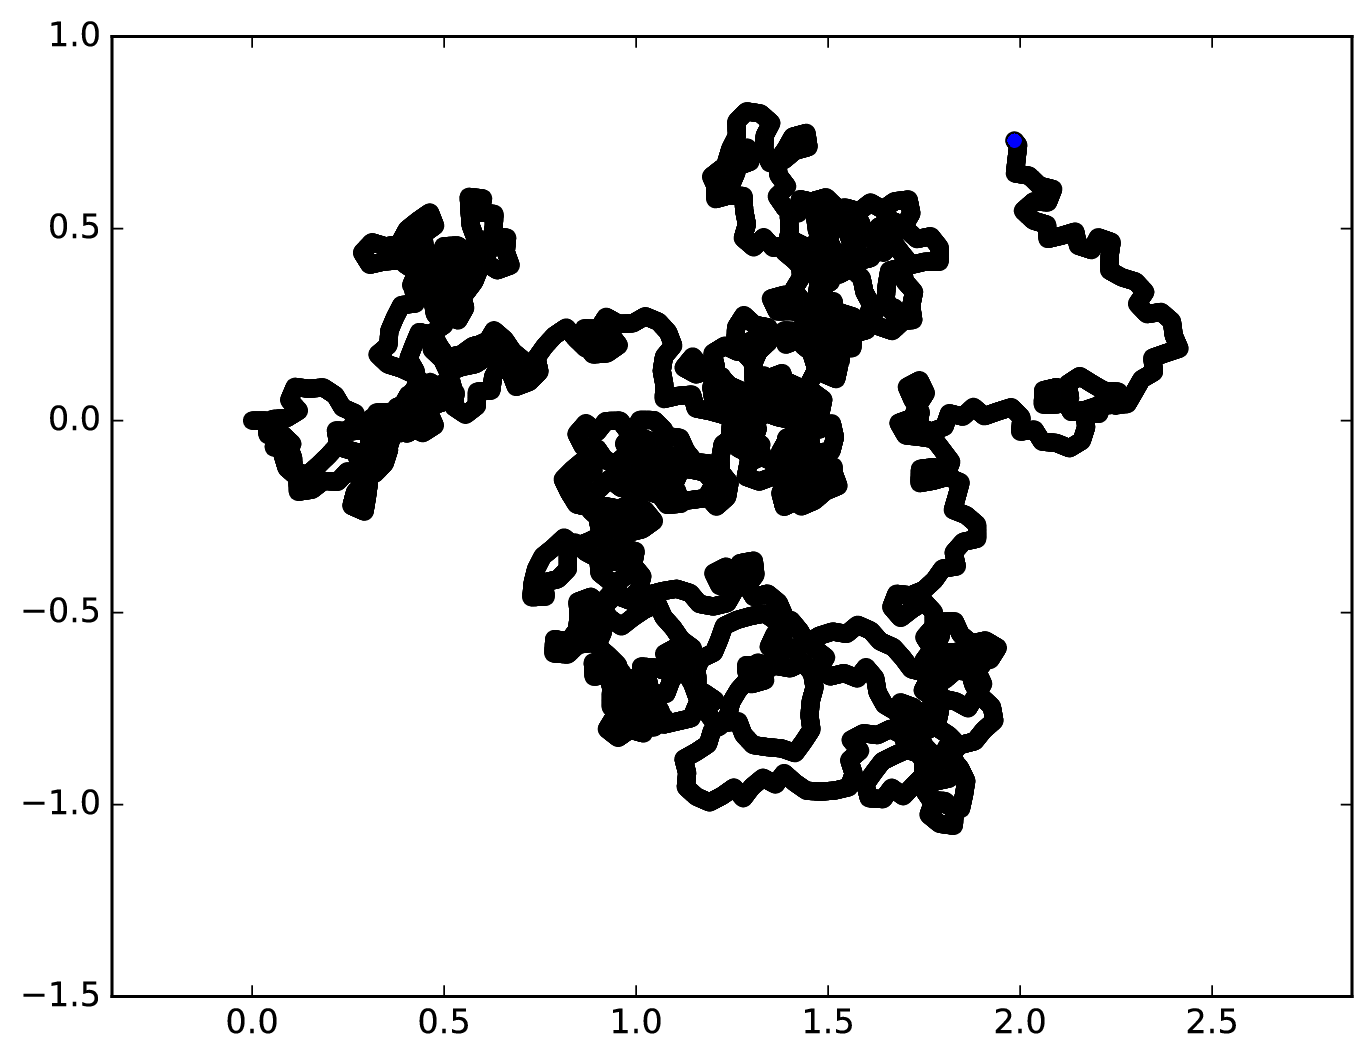
\includegraphics[width=\textwidth]{figures/ch3/synTraj_219_105_60}
			\caption[$A = 105$, $F=60$]{$A = 105$, $F=60$}
			\label{fig:synTraj_219_105_60}
		\end{subfigure}
		~
		\begin{subfigure}[t]{\subImgWmo}
			\centering
			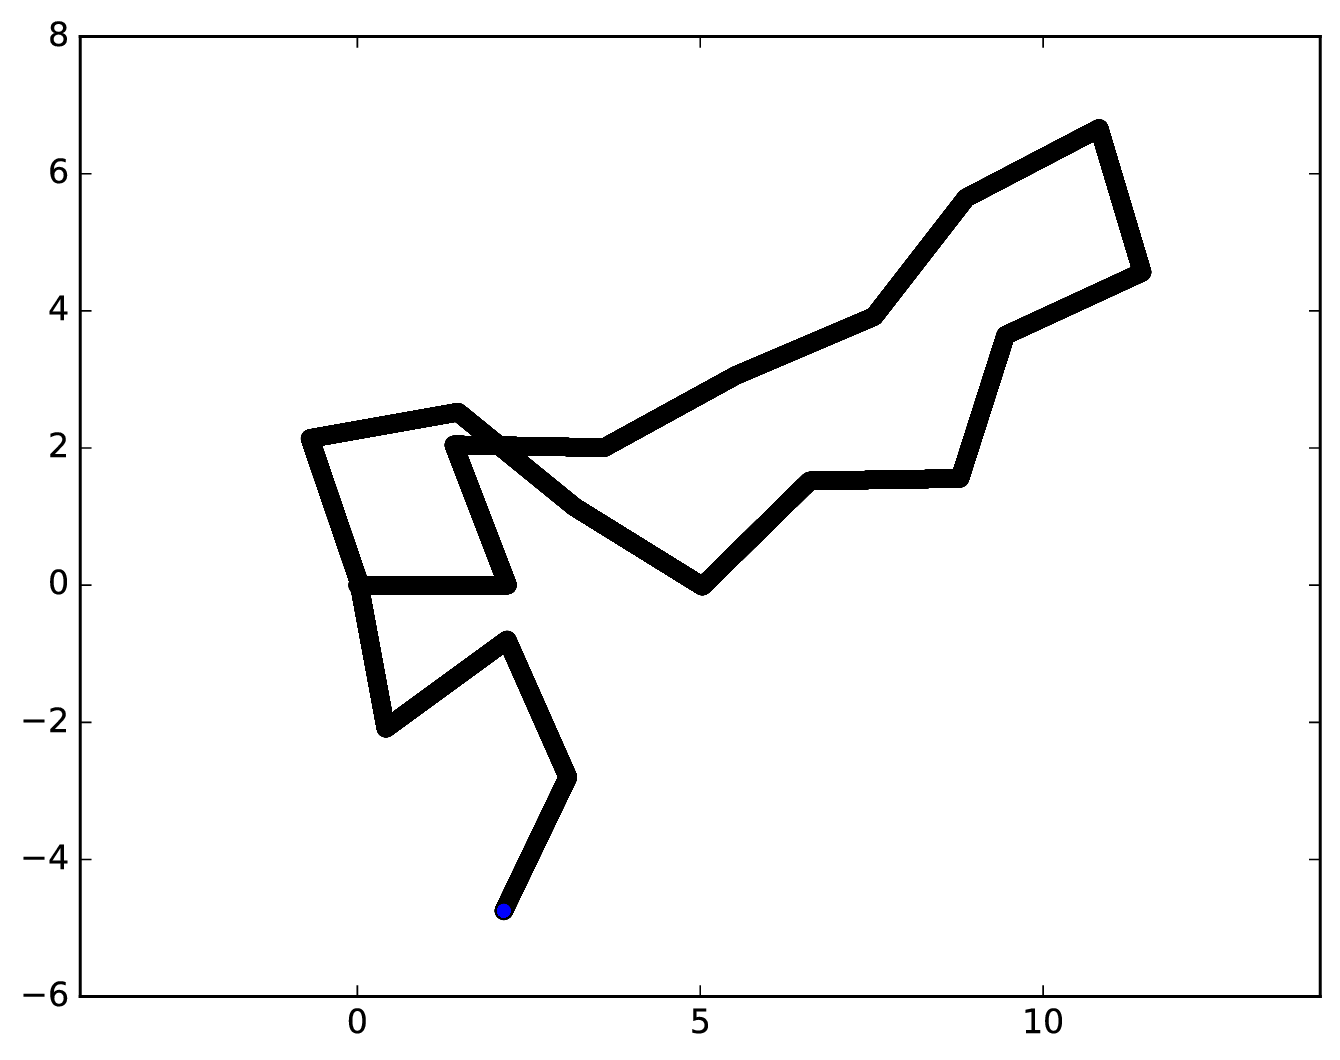
\includegraphics[width=\textwidth]{figures/ch3/synTraj_219_120_1}
			\caption[$A = 120$, $F=1$]{$A = 120$, $F=1$}
			\label{fig:synTraj_219_120_1}
		\end{subfigure}
		~
		\begin{subfigure}[t]{\subImgWmo}
			\centering
			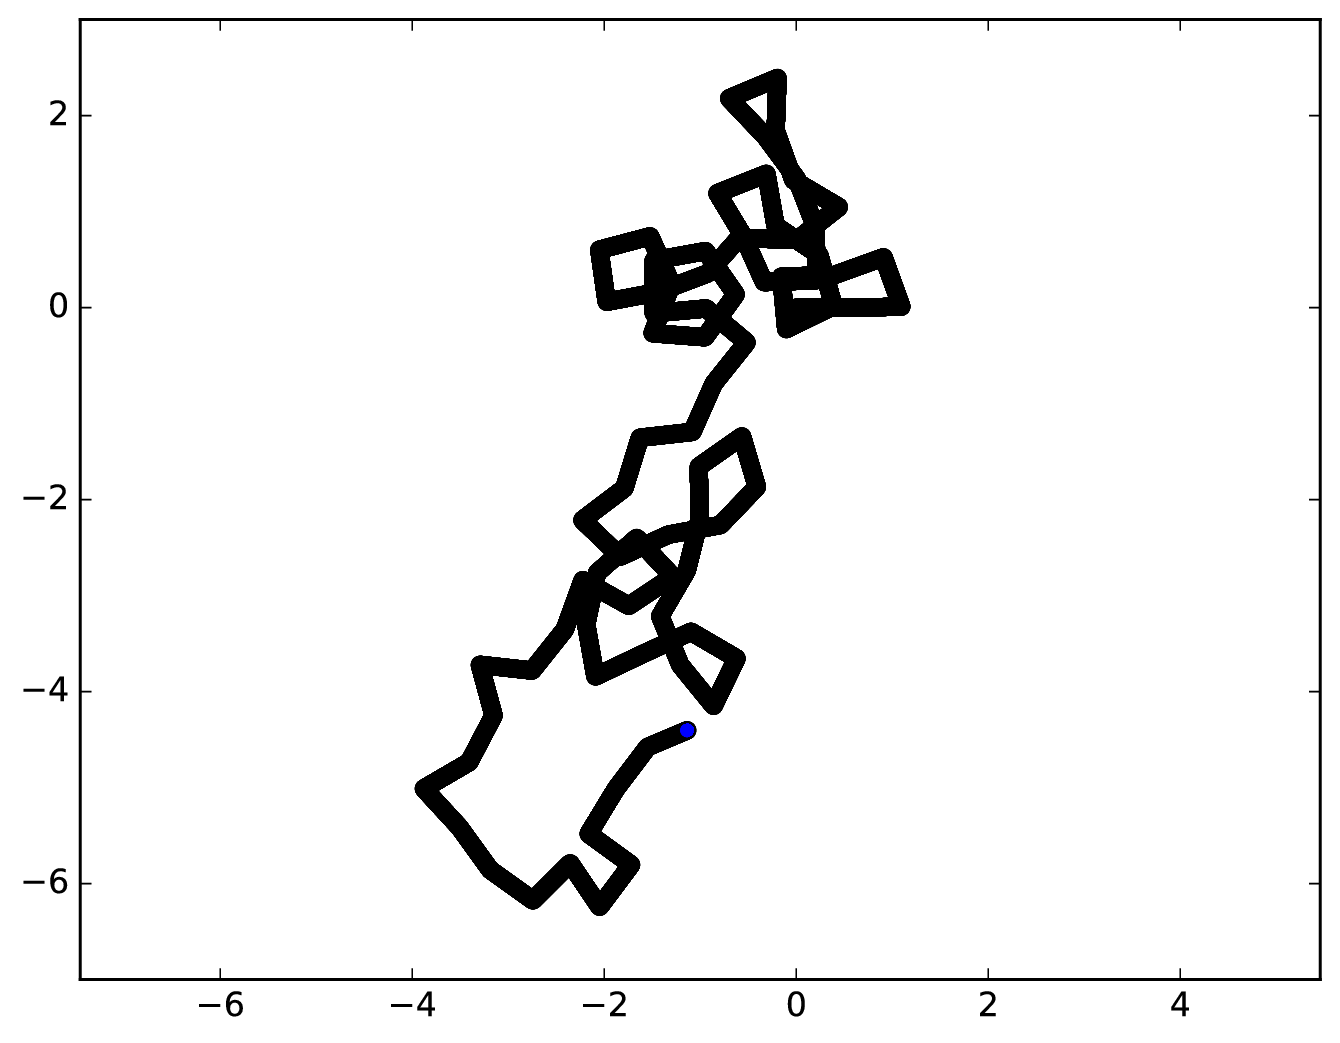
\includegraphics[width=\textwidth]{figures/ch3/synTraj_219_120_4}
			\caption[$A = 120$, $F=4$]{$A = 120$, $F=4$}
			\label{fig:synTraj_219_120_4}
		\end{subfigure}
		~
		\begin{subfigure}[t]{\subImgWmo}
			\centering
			\includegraphics[width=\textwidth]{figures/ch3/synTraj_219_120_8}
			\caption[$A = 120$, $F=8$]{$A = 120$, $F=8$}
			\label{fig:synTraj_219_120_8}
		\end{subfigure}
		~
		\begin{subfigure}[t]{\subImgWmo}
			\centering
			\includegraphics[width=\textwidth]{figures/ch3/synTraj_219_120_16}
			\caption[$A = 120$, $F=16$]{$A = 120$, $F=16$}
			\label{fig:synTraj_219_120_16}
		\end{subfigure}
		~
		\begin{subfigure}[t]{\subImgWmo}
			\centering
			\includegraphics[width=\textwidth]{figures/ch3/synTraj_219_120_32}
			\caption[$A = 120$, $F=32$]{$A = 120$, $F=32$}
			\label{fig:synTraj_219_120_32}
		\end{subfigure}
		~
		\begin{subfigure}[t]{\subImgWmo}
			\centering
			\includegraphics[width=\textwidth]{figures/ch3/synTraj_219_120_60}
			\caption[$A = 120$, $F=60$]{$A = 120$, $F=60$}
			\label{fig:synTraj_219_120_60}
		\end{subfigure}
		\caption[Mouvements générés par notre modèle -- IV]{Exemples de trajectoires générées par notre modèle pour un objet de vitesse constante (2,19~cm/s).}
		\label{fig:motion105120}
	\end{figure}
	
	\subsubsection{Effet combiné des angles et fréquences}
	L'effet des fréquences étant qualitativement comparable à celui des angles, on peut considérer que ces paramètres sont approximativement équivalents et, de fait, les regrouper en un seul par un produit. Ainsi, l'on peut s'intéresser non pas à leurs valeurs respectives mais au produit $AF$, que nous avons également baptisé \emph{pseudo-entropie}.
	
	Insistons sur le fait qu'il s'agit d'une approximation, mais notez que pour une valeur de $AF$ de 480, par exemple, on a les trajectoires de la figure~\ref{fig:synTraj_219_30_16} et celle de la figure~\ref{fig:synTraj_219_120_4}. Bien que visiblement distinctes, ces deux trajectoires présentent un niveau d'irrégularité grossièrement comparable. Pour $AF = 720$, les trajectoires des figures~\ref{fig:synTraj_219_90_8} et~\ref{fig:synTraj_219_45_16} sont également assez semblables.
	
	Notons tout de même que pour une valeur de $AF$ donnée, même si l'irrégularité globale est généralement comparable, une trajectoire générée par une valeur de $F$ relativement élevée tend à être plus lisse et courbée, tandis que quand $A$ domine, elle est plutôt \og saccadée \fg{}.
	
	Ce point sera particulièrement visible avec la même valeur de $AF$ de 180, mais en comparant les trajectoires présentées sur la figure~\ref{fig:trajsAF180}. En effet, si $180 \times 1 = 15 \times 12 = 180$, nous avons dans un cas un $A$ très grand avec un $F$ très petit, et dans l'autre des valeurs plus \og équilibrées \fg{}. Le résultat est une trajectoire très saccadée sur la première trajectoire (figure~\ref{fig:synTraj_219_180_1b}) et plutôt lisse et courbe sur la seconde (figure~\ref{fig:synTraj_219_15_12}).
	
	\begin{figure}[htb]
		\begin{subfigure}[t]{0.49\textwidth}
			\centering
			\includegraphics[width=\textwidth]{figures/ch3/synTraj_219_180_1}
			\caption[$A = 180$, $F=1$]{$A = 180$, $F=1$}
			\label{fig:synTraj_219_180_1b}
		\end{subfigure}
		~
		\begin{subfigure}[t]{0.49\textwidth}
			\centering
			\includegraphics[width=\textwidth]{figures/ch3/synTraj_219_15_12}
			\caption[$A = 15$, $F=12$]{$A = 15$, $F=12$}
			\label{fig:synTraj_219_15_12}
		\end{subfigure}
		\caption[Trajectoires pour $AF = 180$]{Trajectoires pour $AF = 180$ et $S = 2,19~cm/s$. On observe que pour un produit $AF$ donné, si $A$ est particulièrement grand et $F$ particulièrement petit sur une trajectoire (et inversement sur l'autre) les résultats obtenus diffèrent significativement.}
		\label{fig:trajsAF180}
	\end{figure}
	
	
	L'on pourra donc, dans certains cas, utiliser le produit $AF$ seul, pour simplifier l'étude des résultats, mais il convient de le faire en ayant à l'esprit que c'est une approximation, et qu'elle tend à être moins précise pour les valeurs de $A$ ou $F$ particulièrement faibles ou élevées.
	
	\begin{figure}[htb]
		\begin{subfigure}[t]{\subImgWmo}
			\centering
			\includegraphics[width=\textwidth]{figures/ch3/synTraj_219_135_1}
			\caption[$A = 135$, $F=1$]{$A = 135$, $F=1$}
			\label{fig:synTraj_219_135_1}
		\end{subfigure}
		~
		\begin{subfigure}[t]{\subImgWmo}
			\centering
			\includegraphics[width=\textwidth]{figures/ch3/synTraj_219_135_4}
			\caption[$A = 135$, $F=4$]{$A = 135$, $F=4$}
			\label{fig:synTraj_219_135_4}
		\end{subfigure}
		~
		\begin{subfigure}[t]{\subImgWmo}
			\centering
			\includegraphics[width=\textwidth]{figures/ch3/synTraj_219_135_8}
			\caption[$A = 135$, $F=8$]{$A = 135$, $F=8$}
			\label{fig:synTraj_219_135_8}
		\end{subfigure}
		~
		\begin{subfigure}[t]{\subImgWmo}
			\centering
			\includegraphics[width=\textwidth]{figures/ch3/synTraj_219_135_16}
			\caption[$A = 135$, $F=16$]{$A = 135$, $F=16$}
			\label{fig:synTraj_219_135_16}
		\end{subfigure}
		~
		\begin{subfigure}[t]{\subImgWmo}
			\centering
			\includegraphics[width=\textwidth]{figures/ch3/synTraj_219_135_32}
			\caption[$A = 135$, $F=32$]{$A = 135$, $F=32$}
			\label{fig:synTraj_219_135_32}
		\end{subfigure}
		~
		\begin{subfigure}[t]{\subImgWmo}
			\centering
			\includegraphics[width=\textwidth]{figures/ch3/synTraj_219_135_60}
			\caption[$A = 135$, $F=60$]{$A = 135$, $F=60$}
			\label{fig:synTraj_219_135_60}
		\end{subfigure}
		~
		\begin{subfigure}[t]{\subImgWmo}
			\centering
			\includegraphics[width=\textwidth]{figures/ch3/synTraj_219_150_1}
			\caption[$A = 150$, $F=1$]{$A = 150$, $F=1$}
			\label{fig:synTraj_219_150_1}
		\end{subfigure}
		~
		\begin{subfigure}[t]{\subImgWmo}
			\centering
			\includegraphics[width=\textwidth]{figures/ch3/synTraj_219_150_4}
			\caption[$A = 150$, $F=4$]{$A = 150$, $F=4$}
			\label{fig:synTraj_219_150_4}
		\end{subfigure}
		~
		\begin{subfigure}[t]{\subImgWmo}
			\centering
			\includegraphics[width=\textwidth]{figures/ch3/synTraj_219_150_8}
			\caption[$A = 150$, $F=8$]{$A = 150$, $F=8$}
			\label{fig:synTraj_219_150_8}
		\end{subfigure}
		~
		\begin{subfigure}[t]{\subImgWmo}
			\centering
			\includegraphics[width=\textwidth]{figures/ch3/synTraj_219_150_16}
			\caption[$A = 150$, $F=16$]{$A = 150$, $F=16$}
			\label{fig:synTraj_219_150_16}
		\end{subfigure}
		~
		\begin{subfigure}[t]{\subImgWmo}
			\centering
			\includegraphics[width=\textwidth]{figures/ch3/synTraj_219_150_32}
			\caption[$A = 150$, $F=32$]{$A = 150$, $F=32$}
			\label{fig:synTraj_219_150_32}
		\end{subfigure}
		~
		\begin{subfigure}[t]{\subImgWmo}
			\centering
			\includegraphics[width=\textwidth]{figures/ch3/synTraj_219_150_60}
			\caption[$A = 150$, $F=60$]{$A = 150$, $F=60$}
			\label{fig:synTraj_219_150_60}
		\end{subfigure}
		\caption[Mouvements générés par notre modèle -- V]{Exemples de trajectoires générées par notre modèle pour un objet de vitesse constante (2,19~cm/s).}
		\label{fig:motion135150}
	\end{figure}
	
	\subsubsection{Longueur des trajectoires, aires des enveloppes convexes}
	Pour rappel, toutes les trajectoires des figures~\ref{fig:motion1530}, \ref{fig:motion4560}, \ref{fig:motion7590}, \ref{fig:motion105120}, \ref{fig:motion135150} et \ref{fig:motion165180} furent générées par un mouvement de vitesse constante, 2,19~cm/s. Attendu qu'elles ont également été générées sur une même durée (20 secondes) elles ont toutes la même longueur, malgré les apparences dues aux variations d'échelle : $2,19~cm/s \times 20~s = 43,8~cm$.
	
	Mais certaines trajectoires sont très peu \og nouées \fg{} tandis que d'autres le sont beaucoup. De fait, l'espace horizontal ou vertical qu'elles occupent peut varier considérablement. Par exemple, comme nous le mentionnions plus haut,	la trajectoire de la figure~\ref{fig:synTraj_219_15_1} parcourt plus de 40~cm à l'horizontale, tandis que celle de la figure~\ref{fig:synTraj_219_180_60} est contenue dans un rectangle d'environ 1,2~cm de hauteur sur 1~cm de largeur.
	
	En règle générale, plus la pseudo-entropie est faible, plus la trajectoire parcourra une distance horizontale ou verticale importante, et plus la pseudo-entropie est élevée, plus ces distances sont faibles. Notez cependant que cela n'implique pas nécessairement qu'une trajectoire de faible pseudo-entropie occupera forcément une aire importante, car comme le montre la figure~\ref{fig:synTraj_219_30_1}, la distance parcourue sur un axe (vertical, en l'occurrence) peut être très faible.
	
	\begin{figure}[htb]
		\begin{subfigure}[t]{\subImgWmo}
			\centering
			\includegraphics[width=\textwidth]{figures/ch3/synTraj_219_165_1}
			\caption[$A = 165$, $F=1$]{$A = 165$, $F=1$}
			\label{fig:synTraj_219_165_1}
		\end{subfigure}
		~
		\begin{subfigure}[t]{\subImgWmo}
			\centering
			\includegraphics[width=\textwidth]{figures/ch3/synTraj_219_165_4}
			\caption[$A = 165$, $F=4$]{$A = 165$, $F=4$}
			\label{fig:synTraj_219_165_4}
		\end{subfigure}
		~
		\begin{subfigure}[t]{\subImgWmo}
			\centering
			\includegraphics[width=\textwidth]{figures/ch3/synTraj_219_165_8}
			\caption[$A = 165$, $F=8$]{$A = 165$, $F=8$}
			\label{fig:synTraj_219_165_8}
		\end{subfigure}
		~
		\begin{subfigure}[t]{\subImgWmo}
			\centering
			\includegraphics[width=\textwidth]{figures/ch3/synTraj_219_165_16}
			\caption[$A = 165$, $F=16$]{$A = 165$, $F=16$}
			\label{fig:synTraj_219_165_16}
		\end{subfigure}
		~
		\begin{subfigure}[t]{\subImgWmo}
			\centering
			\includegraphics[width=\textwidth]{figures/ch3/synTraj_219_165_32}
			\caption[$A = 165$, $F=32$]{$A = 165$, $F=32$}
			\label{fig:synTraj_219_165_32}
		\end{subfigure}
		~
		\begin{subfigure}[t]{\subImgWmo}
			\centering
			\includegraphics[width=\textwidth]{figures/ch3/synTraj_219_165_60}
			\caption[$A = 165$, $F=60$]{$A = 165$, $F=60$}
			\label{fig:synTraj_219_165_60}
		\end{subfigure}
		~
		\begin{subfigure}[t]{\subImgWmo}
			\centering
			\includegraphics[width=\textwidth]{figures/ch3/synTraj_219_180_1}
			\caption[$A = 180$, $F=1$]{$A = 180$, $F=1$}
			\label{fig:synTraj_219_180_1}
		\end{subfigure}
		~
		\begin{subfigure}[t]{\subImgWmo}
			\centering
			\includegraphics[width=\textwidth]{figures/ch3/synTraj_219_180_4}
			\caption[$A = 180$, $F=4$]{$A = 180$, $F=4$}
			\label{fig:synTraj_219_180_4}
		\end{subfigure}
		~
		\begin{subfigure}[t]{\subImgWmo}
			\centering
			\includegraphics[width=\textwidth]{figures/ch3/synTraj_219_180_8}
			\caption[$A = 180$, $F=1$]{$A = 180$, $F=8$}
			\label{fig:synTraj_219_180_8}
		\end{subfigure}
		~
		\begin{subfigure}[t]{\subImgWmo}
			\centering
			\includegraphics[width=\textwidth]{figures/ch3/synTraj_219_180_16}
			\caption[$A = 180$, $F=16$]{$A = 180$, $F=16$}
			\label{fig:synTraj_219_180_16}
		\end{subfigure}
		~
		\begin{subfigure}[t]{\subImgWmo}
			\centering
			\includegraphics[width=\textwidth]{figures/ch3/synTraj_219_180_32}
			\caption[$A = 180$, $F=32$]{$A = 180$, $F=32$}
			\label{fig:synTraj_219_180_32}
		\end{subfigure}
		~
		\begin{subfigure}[t]{\subImgWmo}
			\centering
			\includegraphics[width=\textwidth]{figures/ch3/synTraj_219_180_60}
			\caption[$A = 180$, $F=60$]{$A = 180$, $F=60$}
			\label{fig:synTraj_219_180_60}
		\end{subfigure}
		\caption[Mouvements générés par notre modèle -- VI]{Exemples de trajectoires générées par notre modèle pour un objet de vitesse constante (2,19~cm/s).}
		\label{fig:motion165180}
	\end{figure}
	
	Une façon d'estimer l'aire de la surface occupée par un ensemble de points (comme une trajectoire) consiste à calculer l'aire de son enveloppe convexe. L'enveloppe convexe d'un ensemble de points du plan est le plus petit polygone convexe contenant tous les points de l'ensemble. Dans un espace en trois dimensions, l'enveloppe convexe est simplement le plus petit polyèdre convexe contenant tous les points de l'ensemble. Des exemples d'enveloppes convexes sont représentés sur la figure~\ref{fig:trajAreas}. On y remarque notamment une relation inverse entre la pseudo-entropie et l'aire de l'enveloppe convexe de la trajectoire. Les trajectoires de pseudo-entropie très faible, telle que celle de la figure~\ref{fig:areaTraj_219_1_16}, occupent un espace important, tandis que les trajectoires de très forte pseudo-entropie, comme celle de la figure~\ref{fig:areaTraj_219_180_240}, sont confinées à une toute petite zone.
	
	
	\begin{figure}[htb]
		\centering
		\begin{subfigure}[t]{\subImgWarea}
			\centering
			\includegraphics[width=\textwidth]{figures/ch3/areaTraj_219_1_16}
			\caption[$A = 1$, $F=16$]{$A = 1$, $F=16$, $AF=16$. L'aire de l'enveloppe est d'environ 87~cm².}
			\label{fig:areaTraj_219_1_16}
		\end{subfigure}
		~
		\begin{subfigure}[t]{\subImgWarea}
			\centering
			\includegraphics[width=\textwidth]{figures/ch3/areaTraj_219_5_16}
			\caption[Enveloppe convexe, $A = 5$, $F=16$]{$A = 5$, $F=16$, $AF=80$. L'aire de l'enveloppe est d'environ 83~cm².}
			\label{fig:areaTraj_219_5_16}
		\end{subfigure}
		~
		\begin{subfigure}[t]{\subImgWarea}
			\centering
			\includegraphics[width=\textwidth]{figures/ch3/areaTraj_219_45_4}
			\caption[Enveloppe convexe, $A = 45$, $F=4$]{$A = 45$, $F=4$, $AF=180$. L'aire de l'enveloppe est d'environ 48~cm².}
			\label{fig:areaTraj_219_45_4}
		\end{subfigure}
		~
		\begin{subfigure}[t]{\subImgWarea}
			\centering
			\includegraphics[width=\textwidth]{figures/ch3/areaTraj_219_90_8}
			\caption[Enveloppe convexe, $A = 90$, $F=8$]{$A = 90$, $F=8$, $AF=720$. L'aire de l'enveloppe est d'environ 16,4~cm².}
			\label{fig:areaTraj_219_90_8}
		\end{subfigure}
		~
		\begin{subfigure}[t]{\subImgWarea}
			\centering
			\includegraphics[width=\textwidth]{figures/ch3/areaTraj_219_180_60}
			\caption[Enveloppe convexe, $A = 180$, $F=60$]{$A = 180$, $F=60$, $AF=10800$. L'aire de l'enveloppe est d'environ 3,25~cm².}
			\label{fig:areaTraj_219_180_60}
		\end{subfigure}
		~
		\begin{subfigure}[t]{\subImgWarea}
			\centering
			\includegraphics[width=\textwidth]{figures/ch3/areaTraj_219_180_240}
			\caption[Enveloppe convexe, $A = 180$, $F=240$]{$A = 180$, $F=240$, $AF=43200$. L'aire de l'enveloppe est d'environ 1,85~cm².}
			\label{fig:areaTraj_219_180_240}
		\end{subfigure}
		\caption[Enveloppes convexes]{Enveloppes convexes de six trajectoires de pseudo-entropies croissantes. À mesure que la pseudo-entropie croît, elles sont de plus en plus \og repliées \fg{} et l'aire de l'enveloppe convexe décroît.}
		\label{fig:trajAreas}
	\end{figure}
	
	L'on peut déduire de cette observation que si un utilisateur souhaite sélectionner une cible mobile de faible pseudo-entropie, il doit pouvoir atteindre, avec son curseur, tous les points d'une zone de taille importante, comme sur la figure~\ref{fig:areaTraj_219_1_16} ; si la pseudo-entropie est élevée, cependant, la zone sera plus petite, comme sur la figure~\ref{fig:areaTraj_219_180_240}). En cas de pseudo-entropie moyenne, enfin, la zone sera de taille intermédiaire, comme l'illustre la figure~\ref{fig:areaTraj_219_90_8}.
	
	Il serait tentant d'en déduire que la pseudo-entropie rend la sélection plus facile, mais n'oublions pas qu'elle implique un mouvement moins régulier, et donc plus imprévisible. Nous reviendrons en détail sur ce point plus loin, mais observons simplement pour le moment que les trajectoires des figures~\ref{fig:areaTraj_219_1_16}, \ref{fig:areaTraj_219_5_16} et \ref{fig:areaTraj_219_45_4} (de pseudo-entropie maximale 180) sont nettement plus régulières --- donc prévisibles --- que la trajectoire de la figure~\ref{fig:areaTraj_219_90_8}, de pseudo-entropie 720. Il serait donc très imprudent de supposer que cette dernière correspond à une cible plus facile à sélectionner.
	
	Remarquons cependant que quand la pseudo-entropie est très faible, la régularité de la trajectoire suggère une sélection relativement aisée ; quand elle est très élevée, la très petite zone couverte par la trajectoire laisse également supposer une sélection assez facile, du fait d'une distance (telle que définie par Fitts~\cite{fitts1954information}) très courte --- à partir du moment où le curseur atteint l'enveloppe convexe de la cible, du moins.
	
\section{Résultats}
	Pour étayer notre taxinomie des cibles mobiles et de leurs environnements, nous nous sommes appuyés sur des mesures quantitatives et objectives des critères les plus importants que nous avons retenus. Nous avons pour cela adopté deux approches complémentaires :
	
	\begin{itemize}
		\item Premièrement, nous avons développé une suite d'outils permettant de traiter des résultats bruts de simulations de dynamique moléculaire (appelés \emph{trajectoires}) afin de mesurer les angles de rotation des vecteurs direction des atomes, et d'analyser ces mesures ;
		\item Deuxièmement, nous avons développé une suite d'outils permettant d'annoter des vidéos contenant des cibles sur lesquelles l'utilisateur peut cliquer afin de marquer leurs positions dans le temps, et d'analyser les résultats.
	\end{itemize}

	Dans le premier cas, de très grandes quantités de données peuvent être traitées, en mesurant les angles en 3D, mais uniquement pour des simulations moléculaires. Dans le second, les vidéos peuvent représenter n'importe quel type de cible, mais nécessitent --- pour le moment --- un traitement manuel. L'ajout d'une méthode de reconnaissance d'objet permettrait de se passer de l'intervention d'un humain, mais devrait être très fiable pour être utilisable.
	
	\subsection{Analyses de \emph{trajectoires} de dynamique moléculaire}
	Une simulation de dynamique moléculaire cherche à déterminer le comportement d'un système sur une durée \emph{réelle} donnée, généralement de l'ordre de la nanoseconde. L'état du système (notamment les positions des atomes) est déterminé pour chaque pas de temps. En pratique, les résultats de la simulation peuvent ensuite être affichés avec un nombre de pas de temps par seconde arbitraire, ce qui implique que les vitesses des cibles dépendent du choix fait pour la visualisation.
	
	De même, les atomes sont susceptibles de changer de direction à chaque pas de temps, et c'est généralement le cas. La fréquence des changements de direction dépend donc également du nombre de pas par seconde lors de l'affichage des résultats.
	
	Les valeurs des angles de rotation des vecteurs direction, elles, sont indépendantes de ce choix, puisqu'il s'agit simplement, pour chaque atome, de l'écart entre son vecteur direction d'un pas à l'autre. C'est donc sur cette valeur que nous nous sommes concentrés, en gardant à l'esprit que la vitesse des cibles et la fréquence des changements de direction sont variables et dépendent du mode d'affichage choisi.
	
	Nous avons ainsi analysé plusieurs systèmes en mesurant tous les angles de rotation, pour chaque pas de la simulation. Pour chaque système, nous avons ensuite dressé un histogramme de toutes ces valeurs, afin d'avoir une représentation complète de toute la gamme d'angles possibles, et des proportions dans lesquelles ils apparaissent. Ces histogrammes sont présentés sur la figure~\ref{fig:dynMolAngles}.
	
	\newcommand{\subImgWaStats}{0.49\textwidth}
	\begin{figure}[htb]
		\begin{subfigure}[t]{\subImgWaStats}
			\centering
			\includegraphics[width=\textwidth]{figures/ch3/02_DA_all_angles}
			\caption{}
			\label{fig:02_DA_all_angles}
		\end{subfigure}
		~
		\begin{subfigure}[t]{\subImgWaStats}
			\centering
			\includegraphics[width=\textwidth]{figures/ch3/148L_all_angles}
			\caption{}
			\label{fig:148L_all_angles}
		\end{subfigure}
		~
		\begin{subfigure}[t]{\subImgWaStats}
			\centering
			\includegraphics[width=\textwidth]{figures/ch3/snare_tmd_gg_all_angles}
			\caption{}
			\label{fig:snare_tmd_gg_all_angles}
		\end{subfigure}
		~
		\begin{subfigure}[t]{\subImgWaStats}
			\centering
			\includegraphics[width=\textwidth]{figures/ch3/gk_extension_all_angles}
			\caption{}
			\label{fig:gk_extension_all_angles}
		\end{subfigure}
		\caption[Angles de rotation, dynamique moléculaire]{Angles de rotation des vecteurs direction des atomes de simulations de dynamique moléculaire.}
		\label{fig:dynMolAngles}
	\end{figure}

	Sur cette figure, l'on constate que les angles mesurés ont généralement une distribution asymétrique, avec un cas particulier sur la figure~\ref{fig:02_DA_all_angles}, dont l'histogramme admet deux pics. Les lois mathématiques précises régissant ces distributions importent moins que leurs conséquences pratiques, qui découlent d'une part de l'intervalle des valeurs possibles ([0,180] sur tous les systèmes que nous avons étudiés), et d'autre part de leurs fréquences d'occurrence respectives.
	
	Premièrement, tous les angles possibles peuvent apparaître, et ce jusqu'à 180\textdegree{}. Non seulement ces très grands angles (assimilables à des demi-tours) ne sont pas rares, mais sur les systèmes des figures~\ref{fig:148L_all_angles} et~\ref{fig:snare_tmd_gg_all_angles}, ils sont même très fréquents, avec des pics très marqués à cet endroit de leurs histogrammes respectifs.
	
	Deuxièmement, les angles les plus fréquents peuvent être autour de 100\textdegree{} (figure~\ref{fig:148L_all_angles}), 130\textdegree{} (figure~\ref{fig:snare_tmd_gg_all_angles}), 140\textdegree{} (figure~\ref{fig:gk_extension_all_angles}) ou seulement 25\textdegree{} (figure~\ref{fig:02_DA_all_angles}).
	
	Par conséquent, l'interaction avec les (résultats de) simulations de dynamique moléculaire nécessite de pouvoir gérer des angles de rotation de n'importe quelle valeur, et même de s'adapter à des distributions pouvant être très différentes, avec des valeurs d'occurrence maximale pouvant prendre n'importe quelle valeur au sein d'un intervalle s'étendant au moins de 25\textdegree{} à 140\textdegree{}. Sur une autre simulation à très haute fréquence (non présentée ici), nous avons même observé un histogramme entièrement borné par les valeurs 15\textdegree{} et 18\textdegree{}.
	
	Bien qu'il soit envisageable d'effectuer de telles analyses sur un très gros échantillon représentatif de \emph{trajectoires} de dynamique moléculaire, afin d'obtenir des statistiques détaillées, ce serait superflu par rapport à nos objectifs, qui consistent à caractériser les besoins de la tâche. Or, il apparaît que si l'on examine cette application au travers du prisme de notre modèle VFA :
	
	\begin{itemize}
		\item toutes les valeurs de V sont possibles, selon le mode d'affichage choisi,
		\item toutes les valeurs de F sont possibles, selon le mode d'affichage choisi,
		\item toutes les valeurs de A sont possibles, selon la nature du système et les paramètres de la simulation.
	\end{itemize}
	
	Par conséquent, les simulations de dynamique moléculaire peuvent potentiellement entrer dans toutes les catégories de mouvement markovien --- voire autocorrélé si la fréquence est suffisamment élevée. Mais surtout, les mouvements susceptibles de poser les plus grandes difficultés de sélection sont possibles dans cette application.
	
	\subsection{Analyses des mouvements d'objets divers}
	Au cours de cette phase, nous avons annoté des vidéos de types très divers pour caractériser quantitativement et objectivement le mouvement de cibles variées. Nous avons ensuite analysé les résultats pour comptabiliser tous les angles de rotation de vecteur direction, toutes les fréquences de rotation, et toutes les vitesses. Nous avons donc pu construire des histogrammes pour chacune de ces grandeurs, mais aussi en calculer la moyenne, l'écart-type, et en noter la valeur maximale.
	
	Avant d'exposer et commenter nos résultats, il convient de noter que les fréquences de changements de direction mesurées ici sont significativement affectées par le nombre d'images par seconde dans les vidéos utilisées comme sources. Celles-ci ont généralement une fréquence de 24~Hz ou 30~Hz, qui peut être insuffisante pour correctement échantillonner les véritables fréquences de changement de direction des cibles observées, si elles dépassent 12~Hz ou 15~Hz, respectivement. La prudence s'impose donc pour l'interprétation de nos résultats concernant cette caractéristique du mouvement ; cette réserve ne s'applique pas aux vitesses, et nettement moins aux angles.
	
	Par ailleurs, la nature intrinsèquement discrète des vidéos, constituées d'un nombre donné d'images par seconde, implique une discrétisation \emph{de facto} de mouvements qui, en soi, peuvent être ciné-continus. La lecture de ces résultats impose de garder à l'esprit qu'ils ne reflètent pas directement la nature réelle des mouvements mesurés. Mais puisque les tâches de sélection impliquent presque toujours un système interactif opérant une discrétisation semblable, nos mesures demeurent pertinentes d'un point de vue pratique et applicatif.
	
	Pour commencer, nous avons annoté un enregistrement vidéo d'une simulation de dynamique moléculaire, avec une petite molécule. Les résultats que nous avons obtenus sont présentés sous forme d'histogrammes de vitesses (figure~\ref{fig:atom_filteredSpeed}), de fréquences (figure~\ref{fig:atom_frequency}), et d'angles (figure~\ref{fig:atom_angle}) d'une part ; et sur la table~\ref{tab:atom_stats} d'autre part. Sur cette dernière et sur toutes les tables de cette section figurent la vitesse maximale enregistrée ($V_{max}$), la vitesse moyenne ($\overline{V}$), l'écart-type des vitesses, ($\sigma_{V}$), la fréquence maximale ($F_{max}$), la fréquence moyenne ($\overline{F}$), l'écart-type des fréquences ($\sigma_{F}$), l'angle maximal ($A_{max}$), l'angle moyen ($\overline{A}$), et enfin l'écart-type des angles ($\sigma_{A}$). Sur les histogrammes comme sur les tables, les vitesses sont en cm/s, les fréquences en Hz, et les angles en degrés. Les résultats sont cohérents avec nos mesures sur des données brutes de simulation, et illustrent bien à quel point les cibles de ce type peuvent être difficiles à saisir.
	
	\newcommand{\subImgWclicks}{0.32\textwidth}
	
	\begin{figure}[!htb]
		\begin{subfigure}[t]{\subImgWclicks}
			\centering
			\includegraphics[width=\textwidth]{figures/ch3/atom_filteredSpeed}
			\caption{Vitesses.}
			\label{fig:atom_filteredSpeed}
		\end{subfigure}
		~
		\begin{subfigure}[t]{\subImgWclicks}
			\centering
			\includegraphics[width=\textwidth]{figures/ch3/atom_frequency}
			\caption{Fréquences.}
			\label{fig:atom_frequency}
		\end{subfigure}
		~
		\begin{subfigure}[t]{\subImgWclicks}
			\centering
			\includegraphics[width=\textwidth]{figures/ch3/atom_angle}
			\caption{Angles.}
			\label{fig:atom_angle}
		\end{subfigure}
		\caption[Histogrammes pour la dynamique moléculaire]{Histogrammes pour la dynamique moléculaire.}
		\label{fig:histAtoms}
	\end{figure}

\begin{table}
	\centering
	\begin{tabular}{c c c c c c c c c}
		$V_{max}$	& $\overline{V}$	& $\sigma_{V}$	& $F_{max}$	& $\overline{F}$	& $\sigma_{F}$	& $A_{max}$	& $\overline{A}$	& $\sigma_{A}$	\bigstrut[b] \\ \hline

		33,08		& 4,84				& 4,60			& 25,00		& 16,82				& 7,20			& 180,00	& 96,98				& 55,86			\bigstrut[t] \\
	\end{tabular}
	\caption[Statistiques pour la vidéo de dynamique moléculaire]{Statistiques pour la vidéo de dynamique moléculaire.}
	\label{tab:atom_stats}
\end{table}	

	Ensuite, nous avons annoté un enregistrement vidéo d'un avion de ligne, filmé depuis le sol avec une caméra suivant l'appareil, tenue à la main, ce qui implique de fréquentes saccades. Les histogrammes correspondants sont sur les figures~\ref{fig:chinaA_filteredSpeed}, \ref{fig:chinaA_frequency}, et \ref{fig:chinaA_angle} ; la table~\ref{tab:chinaA_stats} synthétise ces résultats.

	\begin{figure}[!htb]
		\begin{subfigure}[t]{\subImgWclicks}
			\centering
			\includegraphics[width=\textwidth]{figures/ch3/chinaA_filteredSpeed}
			\caption{Vitesses.}
			\label{fig:chinaA_filteredSpeed}
		\end{subfigure}
		~
		\begin{subfigure}[t]{\subImgWclicks}
			\centering
			\includegraphics[width=\textwidth]{figures/ch3/chinaA_frequency}
			\caption{Fréquences.}
			\label{fig:chinaA_frequency}
		\end{subfigure}
		~
		\begin{subfigure}[t]{\subImgWclicks}
			\centering
			\includegraphics[width=\textwidth]{figures/ch3/chinaA_angle}
			\caption{Angles.}
			\label{fig:chinaA_angle}
		\end{subfigure}
		\caption[Histogrammes pour l'avion de ligne]{Histogrammes pour l'avion de ligne.}
		\label{fig:histChina}
	\end{figure}
	
\begin{table}
	\centering
	\begin{tabular}{c c c c c c c c c}
		$V_{max}$	& $\overline{V}$	& $\sigma_{V}$	& $F_{max}$	& $\overline{F}$	& $\sigma_{F}$	& $A_{max}$	& $\overline{A}$	& $\sigma_{A}$	\bigstrut[b] \\ \hline

		112,36		& 18,21				& 16,26			& 59,96		& 17,50				& 17,39			& 180,00	& 55,42				& 52,50			\bigstrut[t] \\
	\end{tabular}
	\caption[Statistiques pour la vidéo de l'avion de ligne]{Statistiques pour la vidéo de l'avion de ligne.}
	\label{tab:chinaA_stats}
\end{table}

	Les petites vitesses sont majoritaires, notamment car la caméra suit la cible, mais les vitesses élevées sont loin d'être rares, notamment du fait de saccades dans la vidéo. La plupart des angles sont faibles mais l'abondance de saccades mène à une distribution assez \og plate \fg{} une fois les petits angles écartés.

	Sur le même thème, nous avons annoté une vidéo de l'éphémère vol du \emph{Concorde} qui s'écrasa à Gonesse en juillet 2000\footnotemark{}. Les histogrammes sont sur les figures~\ref{fig:concordeA_filteredSpeed}, \ref{fig:concordeA_frequency}, et \ref{fig:concordeA_angle} ; la table~\ref{tab:concordeA_stats} synthétise ces résultats.
		
	\begin{figure}[!htb]
		\begin{subfigure}[t]{\subImgWclicks}
			\centering
			\includegraphics[width=\textwidth]{figures/ch3/concordeA_filteredSpeed}
			\caption{Vitesses.}
			\label{fig:concordeA_filteredSpeed}
		\end{subfigure}
		~
		\begin{subfigure}[t]{\subImgWclicks}
			\centering
			\includegraphics[width=\textwidth]{figures/ch3/concordeA_frequency}
			\caption{Fréquences.}
			\label{fig:concordeA_frequency}
		\end{subfigure}
		~
		\begin{subfigure}[t]{\subImgWclicks}
			\centering
			\includegraphics[width=\textwidth]{figures/ch3/concordeA_angle}
			\caption{Angles.}
			\label{fig:concordeA_angle}
		\end{subfigure}
		\caption[Histogrammes pour le \emph{Concorde}]{Histogrammes pour le \emph{Concorde}.}
		\label{fig:histConcorde}
	\end{figure}
	
	Ici encore et pour les mêmes raisons, les vitesses faibles sont majoritaires mais de nombreuses valeurs élevées furent enregistrées. Les angles sont le plus souvent petits mais parfois beaucoup plus grands. De même, les valeurs proches de 180\textdegree{} s'expliquent par le fait que la caméra peut se déplacer plus vite que la cible, ce qui implique un demi-tour apparent pour celle-ci.
	
	\footnotetext{\url{https://www.bea.aero/docspa/2000/f-sc000725/pdf/f-sc000725.pdf}}

\begin{table}
	\centering
	\begin{tabular}{c c c c c c c c c}
		$V_{max}$	& $\overline{V}$	& $\sigma_{V}$	& $F_{max}$	& $\overline{F}$	& $\sigma_{F}$	& $A_{max}$	& $\overline{A}$	& $\sigma_{A}$	\bigstrut[b] \\ \hline

		29,82		& 6,50				& 4,76			& 25,00		& 12,64				& 8,00			& 176,15	& 48,76				& 48,45			\bigstrut[t] \\
	\end{tabular}
	\caption[Statistiques pour la vidéo du \emph{Concorde}]{Statistiques pour la vidéo du \emph{Concorde}.}
	\label{tab:concordeA_stats}
\end{table}

	Nous soulignions au cours du chapitre~\ref{chap1} l'intérêt des mouvements de foule --- manifestations, émeutes, etc. Aussi avons-nous annoté deux vidéos d'émeutes, dont les histogrammes sont représentés sur la figure~\ref{fig:histRiots}, et dont les résultats synthétiques sont sur les tables~\ref{tab:riot_stats} et \ref{tab:riot2a_stats}.

	\begin{figure}[!htb]
		\begin{subfigure}[t]{\subImgWclicks}
			\centering
			\includegraphics[width=\textwidth]{figures/ch3/riot_filteredSpeed}
			\caption{Vitesses pour l'émeute 1.}
			\label{fig:riot_filteredSpeed}
		\end{subfigure}
		~
		\begin{subfigure}[t]{\subImgWclicks}
			\centering
			\includegraphics[width=\textwidth]{figures/ch3/riot_frequency}
			\caption{Fréquences pour l'émeute 1.}
			\label{fig:riot_frequency}
		\end{subfigure}
		~
		\begin{subfigure}[t]{\subImgWclicks}
			\centering
			\includegraphics[width=\textwidth]{figures/ch3/riot_angle}
			\caption{Angles pour l'émeute 1.}
			\label{fig:riot_angle}
		\end{subfigure}
		~
		\begin{subfigure}[t]{\subImgWclicks}
			\centering
			\includegraphics[width=\textwidth]{figures/ch3/riot2a_filteredSpeed}
			\caption{Vitesses pour l'émeute 2.}
			\label{fig:riot2a_filteredSpeed}
		\end{subfigure}
		~
		\begin{subfigure}[t]{\subImgWclicks}
			\centering
			\includegraphics[width=\textwidth]{figures/ch3/riot2a_frequency}
			\caption{Fréquences pour l'émeute 2.}
			\label{fig:riot2a_frequency}
		\end{subfigure}
		~
		\begin{subfigure}[t]{\subImgWclicks}
			\centering
			\includegraphics[width=\textwidth]{figures/ch3/riot2a_angle}
			\caption{Angles pour l'émeute 2.}
			\label{fig:riot2a_angle}
		\end{subfigure}
		\caption[Histogrammes, émeutes]{}
		\label{fig:histRiots}
	\end{figure}

	Sur ces vidéos, les vitesses sont un peu plus faibles, les valeurs plus élevées étant généralement liées aux charges et autres courses rapides. Les fréquences sont plutôt basses et les angles distribués de façon approximativement uniforme, exception faite des petits angles, sur-représentés, comme c'est souvent le cas.
	
\begin{table}
	\centering
	\begin{tabular}{c c c c c c c c c}
		$V_{max}$	& $\overline{V}$	& $\sigma_{V}$	& $F_{max}$	& $\overline{F}$	& $\sigma_{F}$	& $A_{max}$	& $\overline{A}$	& $\sigma_{A}$	\bigstrut[b] \\ \hline

		43,14		& 3,86				& 3,93			& 25,00		& 4,37				& 5,42			& 180,00	& 75,87				& 54,49			\bigstrut[t] \\
	\end{tabular}
	\caption[Statistiques pour la vidéo d'émeute 1]{Statistiques pour la vidéo d'émeute 1.}
	\label{tab:riot_stats}
\end{table}

	Les deux vidéos produisent des résultats assez cohérents entre eux, ce qui est logique attendu qu'il s'agit d'événements du même type, même si toute émeute est différente des autres.

\begin{table}
	\centering
	\begin{tabular}{c c c c c c c c c}
		$V_{max}$	& $\overline{V}$	& $\sigma_{V}$	& $F_{max}$	& $\overline{F}$	& $\sigma_{F}$	& $A_{max}$	& $\overline{A}$	& $\sigma_{A}$	\bigstrut[b] \\ \hline

		34,47		& 7,54				& 4,36			& 29,97		& 6,47				& 5,41			& 180,00	& 64,57				& 59,56			\bigstrut[t] \\
	\end{tabular}
	\caption[Statistiques pour la vidéo d'émeute 2]{Statistiques pour la vidéo d'émeute 2.}
	\label{tab:riot2a_stats}
\end{table}

	Le contrôle du trafic aérien est une application doublement intéressante : d'une part du fait des caractéristiques de ses cibles, et d'autre part du fait de son caractère critique ; c'est pourquoi nous avons choisi d'en annoter plusieurs vidéos. Pour deux d'entre elles, les histogrammes sont présentés sur la figure~\ref{fig:histAirControl12}, tandis que les statistiques synthétiques sont disponibles dans les tables~\ref{tab:mhA_stats} et \ref{tab:germanwingsA_stats}.
	
	\begin{figure}[!htb]
		\begin{subfigure}[t]{\subImgWclicks}
			\centering
			\includegraphics[width=\textwidth]{figures/ch3/mhA_filteredSpeed}
			\caption{Vitesses, trafic aérien 1.}
			\label{fig:mhA_filteredSpeed}
		\end{subfigure}
		~
		\begin{subfigure}[t]{\subImgWclicks}
			\centering
			\includegraphics[width=\textwidth]{figures/ch3/mhA_frequency}
			\caption{Fréquences, trafic aérien 1.}
			\label{fig:mhA_frequency}
		\end{subfigure}
		~
		\begin{subfigure}[t]{\subImgWclicks}
			\centering
			\includegraphics[width=\textwidth]{figures/ch3/mhA_angle}
			\caption{Angles, trafic aérien 1.}
			\label{fig:mhA_angle}
		\end{subfigure}
		~
		\begin{subfigure}[t]{\subImgWclicks}
			\centering
			\includegraphics[width=\textwidth]{figures/ch3/germanwingsA_filteredSpeed}
			\caption{Vitesses, trafic aérien 2.}
			\label{fig:germanwingsA_filteredSpeed}
		\end{subfigure}
		~
		\begin{subfigure}[t]{\subImgWclicks}
			\centering
			\includegraphics[width=\textwidth]{figures/ch3/germanwingsA_frequency}
			\caption{Fréquences, trafic aérien 2.}
			\label{fig:germanwingsA_frequency}
		\end{subfigure}
		~
		\begin{subfigure}[t]{\subImgWclicks}
			\centering
			\includegraphics[width=\textwidth]{figures/ch3/germanwingsA_angle}
			\caption{Angles, trafic aérien 2.}
			\label{fig:germanwingsA_angle}
		\end{subfigure}
		\caption[Histogrammes, contrôle du trafic aérien]{}
		\label{fig:histAirControl12}
	\end{figure}
	
	Les vitesses sont généralement très basses et stables, ce qui est logique puisque les avions sont observés sur une très grande échelle, et en vol de croisière. Toutefois, elles sont parfois très élevées, en particulier quand le point de vue est déplacé ou en cas de zoom ; c'est là qu'il faut chercher l'explication du second pic, à 5~cm/s, sur la figure~\ref{fig:germanwingsA_filteredSpeed}.
	
	Pour les mêmes raisons, les fréquences sont assez faibles, mais les grands angles ne sont pas rares, même si les petits sont largement majoritaires. Là encore, la raison est essentiellement à chercher du côté des ajustements du point de vue.
	
\begin{table}
	\centering
	\begin{tabular}{c c c c c c c c c}
		$V_{max}$	& $\overline{V}$	& $\sigma_{V}$	& $F_{max}$	& $\overline{F}$	& $\sigma_{F}$	& $A_{max}$	& $\overline{A}$	& $\sigma_{A}$	\bigstrut[b] \\ \hline

		39,69		& 1,82				& 2,79			& 10,00		& 4,23				& 3,13			& 180,00	& 52,68				& 56,62			\bigstrut[t] \\
	\end{tabular}
	\caption[Statistiques pour la vidéo de trafic aérien 1]{Statistiques pour la vidéo de trafic aérien 1.}
	\label{tab:mhA_stats}
\end{table}

\begin{table}
	\centering
	\begin{tabular}{c c c c c c c c c}
		$V_{max}$	& $\overline{V}$	& $\sigma_{V}$	& $F_{max}$	& $\overline{F}$	& $\sigma_{F}$	& $A_{max}$	& $\overline{A}$	& $\sigma_{A}$	\bigstrut[b] \\ \hline

		7,42		& 3,26				& 2,24			& 10,00		& 3,60				& 2,34			& 180,00	& 37,76				& 45,05			\bigstrut[t] \\
	\end{tabular}
	\caption[Statistiques pour la vidéo de trafic aérien 2]{Statistiques pour la vidéo de trafic aérien 2.}
	\label{tab:germanwingsA_stats}
\end{table}

	Nous avons annoté deux vidéos de plus pour le trafic aérien, dont les histogrammes sont sur la figure~\ref{fig:histAirControl34} et les statistiques synthétiques sur les tables~\ref{tab:hkg_stats} et \ref{tab:flightradar2a_stats}.
	
	\begin{figure}[!htb]
		\begin{subfigure}[t]{\subImgWclicks}
			\centering
			\includegraphics[width=\textwidth]{figures/ch3/hkg_filteredSpeed}
			\caption{Vitesses, trafic aérien 3.}
			\label{fig:hkg_filteredSpeed}
		\end{subfigure}
		~
		\begin{subfigure}[t]{\subImgWclicks}
			\centering
			\includegraphics[width=\textwidth]{figures/ch3/hkg_frequency}
			\caption{Fréquences, trafic aérien 3.}
			\label{fig:hkg_frequency}
		\end{subfigure}
		~
		\begin{subfigure}[t]{\subImgWclicks}
			\centering
			\includegraphics[width=\textwidth]{figures/ch3/hkg_angle}
			\caption{Angles, trafic aérien 3.}
			\label{fig:hkg_angle}
		\end{subfigure}
		~
		\begin{subfigure}[t]{\subImgWclicks}
			\centering
			\includegraphics[width=\textwidth]{figures/ch3/flightradar2a_filteredSpeed}
			\caption{Vitesses, trafic aérien 4.}
			\label{fig:flightradar2a_filteredSpeed}
		\end{subfigure}
		~
		\begin{subfigure}[t]{\subImgWclicks}
			\centering
			\includegraphics[width=\textwidth]{figures/ch3/flightradar2a_frequency}
			\caption{Fréquences, trafic aérien 4.}
			\label{fig:flightradar2a_frequency}
		\end{subfigure}
		~
		\begin{subfigure}[t]{\subImgWclicks}
			\centering
			\includegraphics[width=\textwidth]{figures/ch3/flightradar2a_angle}
			\caption{Angles, trafic aérien 4.}
			\label{fig:flightradar2a_angle}
		\end{subfigure}
		\caption[Histogrammes, contrôle du trafic aérien, bis]{}
		\label{fig:histAirControl34}
	\end{figure}
	
	Les résultats sont cohérents avec ceux des vidéos précédentes, ce qui nous fournit une caractérisation assez complète et précise des tâches de sélection de cibles mobiles pour le contrôle du trafic aérien. Certes, ces vidéos sont issues d'outils publics tels que \emph{FlightRadar24} plutôt que d'applications professionnelles, mais le fonctionnement des premiers est proche de celui des secondes.
	
\begin{table}
	\centering
	\begin{tabular}{c c c c c c c c c}
		$V_{max}$	& $\overline{V}$	& $\sigma_{V}$	& $F_{max}$	& $\overline{F}$	& $\sigma_{F}$	& $A_{max}$	& $\overline{A}$	& $\sigma_{A}$	\bigstrut[b] \\ \hline

		4,21		& 1,64				& 0,99			& 30,00		& 3,29				& 4,85			& 176,63	& 53,24				& 52,95			\bigstrut[t] \\
	\end{tabular}
	\caption[Statistiques pour la vidéo  de trafic aérien 3]{Statistiques pour la vidéo  de trafic aérien 3.}
	\label{tab:hkg_stats}
\end{table}

	Il ressort de ces observations que les cibles ne sont pas intrinsèquement très difficiles à sélectionner avec ces outils, mais par leur nombre, la densité et l'occultation qui en résultent, elles peuvent présenter des difficultés significatives. Ajoutons, après avoir consulté la table~\ref{tab:flightradar2a_stats}, que les vitesses maximales peuvent être élevées, notamment lors de modifications du point de vue ou zooms.

\begin{table}
	\centering
	\begin{tabular}{c c c c c c c c c}
		$V_{max}$	& $\overline{V}$	& $\sigma_{V}$	& $F_{max}$	& $\overline{F}$	& $\sigma_{F}$	& $A_{max}$	& $\overline{A}$	& $\sigma_{A}$	\bigstrut[b] \\ \hline

		120,00		& 1,01				& 5,29			& 10,00		& 1,30				& 1,96			& 180,00	& 54,65				& 47,58			\bigstrut[t] \\
	\end{tabular}
	\caption[Statistiques pour la vidéo  de trafic aérien 4]{Statistiques pour la vidéo de trafic aérien 4.}
	\label{tab:flightradar2a_stats}
\end{table}

	Outre l'effet perturbant que de tels pics de vitesse peuvent avoir, notamment par la discontinuité qu'ils introduisent, ils rendent une éventuelle tâche de sélection bien plus difficile, ne serait-ce que ponctuellement.
	
	Les avions ne sont pas les seuls objets volants pouvant faire l'objet d'une tâche de sélection, et c'est pourquoi nous avons aussi annoté une vidéo de la navette spatiale américaine (\emph{Space shuttle} ou \emph{Space Transportation System}, STS). Les histogrammes correspondants sont sur la figure~\ref{fig:histSpace}, tandis que les statistiques synthétiques sont dans la table~\ref{tab:spaceA_stats}.
	
	\begin{figure}[!htb]
		\begin{subfigure}[t]{\subImgWclicks}
			\centering
			\includegraphics[width=\textwidth]{figures/ch3/spaceA_filteredSpeed}
			\caption{Vitesses.}
			\label{fig:spaceA_filteredSpeed}
		\end{subfigure}
		~
		\begin{subfigure}[t]{\subImgWclicks}
			\centering
			\includegraphics[width=\textwidth]{figures/ch3/spaceA_frequency}
			\caption{Fréquences.}
			\label{fig:spaceA_frequency}
		\end{subfigure}
		~
		\begin{subfigure}[t]{\subImgWclicks}
			\centering
			\includegraphics[width=\textwidth]{figures/ch3/spaceA_angle}
			\caption{Angles.}
			\label{fig:spaceA_angle}
		\end{subfigure}
		\caption[Histogrammes pour la navette spatiale]{Histogrammes pour la navette spatiale.}
		\label{fig:histSpace}
	\end{figure}
	
\begin{table}
	\centering
	\begin{tabular}{c c c c c c c c c}
		$V_{max}$	& $\overline{V}$	& $\sigma_{V}$	& $F_{max}$	& $\overline{F}$	& $\sigma_{F}$	& $A_{max}$	& $\overline{A}$	& $\sigma_{A}$	\bigstrut[b] \\ \hline

		382,43		& 25,64				& 27,26			& 29,97		& 8,05				& 7,98			& 180,00	& 65,52				& 55,93			\bigstrut[t] \\
	\end{tabular}
	\caption[Statistiques pour la vidéo de la navette spatiale]{Statistiques pour la vidéo de la navette spatiale.}
	\label{tab:spaceA_stats}
\end{table}
	
	La distribution des vitesses est caractéristique des vidéos de ce type : dominée par les petites valeurs, avec quelques grandes valeurs liées aux saccades de la vidéo. Les fréquences présentent également un profil habituel, mais la distribution des angles est plus intéressante par son caractère relativement équilibré, avec beaucoup de grands angles, malgré une majorité de petits --- d'où des phases de mouvement assez diversifiées.
	
	Dans le domaine aérien, mais cette fois-ci vivant, nous avons annoté une vidéo d'un court vol d'oiseau (un pigeon), dont les histogrammes sont sur la figure~\ref{fig:histOiseau}, et les statistiques synthétiques dans la table~\ref{tab:oiseau_stats}. Les oiseaux en particulier, et les animaux en général pourraient faire l'objet de tâches de sélection de cible mobile dans des applications de réalité augmentée permettant de choisir un individu pour que le système reconnaisse automatiquement son espèce, sa race, et affiche des informations complémentaires tirées d'une base de données, voire d'une encyclopédie en ligne.
		
	\begin{figure}[!htb]
		\begin{subfigure}[t]{\subImgWclicks}
			\centering
			\includegraphics[width=\textwidth]{figures/ch3/oiseau_filteredSpeed}
			\caption{Vitesses.}
			\label{fig:oiseau_filteredSpeed}
		\end{subfigure}
		~
		\begin{subfigure}[t]{\subImgWclicks}
			\centering
			\includegraphics[width=\textwidth]{figures/ch3/oiseau_frequency}
			\caption{Fréquences.}
			\label{fig:oiseau_frequency}
		\end{subfigure}
		~
		\begin{subfigure}[t]{\subImgWclicks}
			\centering
			\includegraphics[width=\textwidth]{figures/ch3/oiseau_angle}
			\caption{Angles.}
			\label{fig:oiseau_angle}
		\end{subfigure}
		\caption[Histogrammes pour le pigeon]{Histogrammes pour le pigeon.}
		\label{fig:histOiseau}
	\end{figure}
	
\begin{table}
	\centering
	\begin{tabular}{c c c c c c c c c}
		$V_{max}$	& $\overline{V}$	& $\sigma_{V}$	& $F_{max}$	& $\overline{F}$	& $\sigma_{F}$	& $A_{max}$	& $\overline{A}$	& $\sigma_{A}$	\bigstrut[b] \\ \hline

		37,77		& 7,88				& 6,10			& 29,97		& 5,10				& 3,90			& 180,00	& 50,36				& 50,74			\bigstrut[t] \\
	\end{tabular}
	\caption[Statistiques pour la vidéo du pigeon]{Statistiques pour la vidéo du pigeon.}
	\label{tab:oiseau_stats}
\end{table}

	Suivi par la caméra, le volatile génère surtout d'assez petites vitesses, d'autant que la vidéo est au ralenti. Ses distributions de fréquences et d'angles indiquent un mouvement de faible pseudo-entropie, donc relativement prévisible.
	
	Pour compléter ces données, nous avons annoté une deuxième courte vidéo du même type : le décollage d'un petit oiseau au ralenti. Les histogrammes sont sur la figure~\ref{fig:histBird}, et les statistiques synthétiques dans la table~\ref{tab:bird_stats}.
	
	\begin{figure}[!htb]
		\begin{subfigure}[t]{\subImgWclicks}
			\centering
			\includegraphics[width=\textwidth]{figures/ch3/bird_filteredSpeed}
			\caption{Vitesses.}
			\label{fig:bird_filteredSpeed}
		\end{subfigure}
		~
		\begin{subfigure}[t]{\subImgWclicks}
			\centering
			\includegraphics[width=\textwidth]{figures/ch3/bird_frequency}
			\caption{Fréquences.}
			\label{fig:bird_frequency}
		\end{subfigure}
		~
		\begin{subfigure}[t]{\subImgWclicks}
			\centering
			\includegraphics[width=\textwidth]{figures/ch3/bird_angle}
			\caption{Angles.}
			\label{fig:bird_angle}
		\end{subfigure}
		\caption[Histogrammes pour le petit oiseau]{Histogrammes pour le petit oiseau.}
		\label{fig:histBird}
	\end{figure}
	
\begin{table}
	\centering
	\begin{tabular}{c c c c c c c c c}
		$V_{max}$	& $\overline{V}$	& $\sigma_{V}$	& $F_{max}$	& $\overline{F}$	& $\sigma_{F}$	& $A_{max}$	& $\overline{A}$	& $\sigma_{A}$	\bigstrut[b] \\ \hline

		37,52		& 8,76				& 8,07			& 23,98		& 9,92				& 9,74			& 171,44	& 60,51				& 50,82			\bigstrut[t] \\
	\end{tabular}
	\caption[Statistiques pour la vidéo du petit oiseau]{Statistiques pour la vidéo du petit oiseau.}
	\label{tab:bird_stats}
\end{table}

	Les résultats sont tout à fait cohérents avec ceux du pigeon, ce qui est logique attendu que les deux vidéos montrent un décollage, sont courtes, et filmées au ralenti.

	Dans la même veine que les oiseaux, et pour les mêmes raisons, nous avons annoté une vidéo d'un poisson dans un aquarium, face à une caméra fixe. Les histogrammes sont présentés sur la figure~\ref{fig:histPoisson}, et les statistiques synthétiques peuvent être consultées dans la table~\ref{tab:poisson_stats}.
	
	\begin{figure}[!htb]
		\begin{subfigure}[t]{\subImgWclicks}
			\centering
			\includegraphics[width=\textwidth]{figures/ch3/poisson_filteredSpeed}
			\caption{Vitesses.}
			\label{fig:poisson_filteredSpeed}
		\end{subfigure}
		~
		\begin{subfigure}[t]{\subImgWclicks}
			\centering
			\includegraphics[width=\textwidth]{figures/ch3/poisson_frequency}
			\caption{Fréquences.}
			\label{fig:poisson_frequency}
		\end{subfigure}
		~
		\begin{subfigure}[t]{\subImgWclicks}
			\centering
			\includegraphics[width=\textwidth]{figures/ch3/poisson_angle}
			\caption{Angles.}
			\label{fig:poisson_angle}
		\end{subfigure}
		\caption[Histogrammes pour le poisson]{Histogrammes pour le poisson.}
		\label{fig:histPoisson}
	\end{figure}
	
\begin{table}
	\centering
	\begin{tabular}{c c c c c c c c c}
		$V_{max}$	& $\overline{V}$	& $\sigma_{V}$	& $F_{max}$	& $\overline{F}$	& $\sigma_{F}$	& $A_{max}$	& $\overline{A}$	& $\sigma_{A}$	\bigstrut[b] \\ \hline

		101,05		& 14,66				& 11,37			& 30,00		& 10,40				& 9,38			& 179,41	& 59,79				& 51,17			\bigstrut[t] \\
	\end{tabular}
	\caption[Statistiques pour la vidéo du poisson]{Statistiques pour la vidéo du poisson.}
	\label{tab:poisson_stats}
\end{table}

	Sans surprise, les vitesses sont généralement faibles, mais on constate une part non négligeable de vitesses relativement élevées (au-delà de 20~cm/s) intéressantes en ce qu'elles ne peuvent être imputées aux mouvements de la caméra, attendu que celle-ci était statique. Malgré une majorité de petits angles, on en trouve beaucoup de grands, encore une fois uniquement liés aux mouvements du poisson.	
	
	Le jeu vidéo fait partie des principales applications impliquant de difficiles tâches de sélection de cibles mobiles ; aussi en avons-nous annoté quelques vidéos, en commençant par une scène d'\emph{Empires of the Undergrowth}, un jeu de tactique en temps réel. Les histogrammes correspondants sont sur la figure~\ref{fig:histSpider}, et les statistiques de synthèse dans la table~\ref{tab:spider_stats}.

	\begin{figure}[!htb]
		\begin{subfigure}[t]{\subImgWclicks}
			\centering
			\includegraphics[width=\textwidth]{figures/ch3/spider_filteredSpeed}
			\caption{Vitesses.}
			\label{fig:spider_filteredSpeed}
		\end{subfigure}
		~
		\begin{subfigure}[t]{\subImgWclicks}
			\centering
			\includegraphics[width=\textwidth]{figures/ch3/spider_frequency}
			\caption{Fréquences.}
			\label{fig:spider_frequency}
		\end{subfigure}
		~
		\begin{subfigure}[t]{\subImgWclicks}
			\centering
			\includegraphics[width=\textwidth]{figures/ch3/spider_angle}
			\caption{Angles.}
			\label{fig:spider_angle}
		\end{subfigure}
		\caption[Histogrammes pour le jeu \emph{Empires of the Undergrowth}]{Histogrammes pour le jeu \emph{Empires of the Undergrowth}.}
		\label{fig:histSpider}
	\end{figure}

\begin{table}
	\centering
	\begin{tabular}{c c c c c c c c c}
		$V_{max}$	& $\overline{V}$	& $\sigma_{V}$	& $F_{max}$	& $\overline{F}$	& $\sigma_{F}$	& $A_{max}$	& $\overline{A}$	& $\sigma_{A}$	\bigstrut[b] \\ \hline

		232,18		& 10,52				& 17,29			& 29,97		& 17,94				& 11,29			& 180,00	& 68,62				& 63,39			\bigstrut[t] \\
	\end{tabular}
	\caption[Statistiques pour la vidéo du jeu \emph{Empires of the Undergrowth}]{Statistiques pour la vidéo du jeu \emph{Empires of the Undergrowth}.}
	\label{tab:spider_stats}
\end{table}

	Si les vitesses ne sont pas énormes, elles dépassent occasionnellement la dizaine de cm/s (ce qui peut être dû à un déplacement du point de vue du joueur) avec de rares valeurs très élevées. Les fréquences sont dominées par un pic à 30~Hz, lié au taux d'images par seconde de la vidéo, et les angles sont caractérisés par deux pics, un à 0\textdegree{} et un à 180\textdegree{}, avec des deux côtés une douce décroissance vers le minimum, autour de 100\textdegree{}. Cela s'explique par les mouvements des créatures de ce jeu, principalement rectilignes avec des virages nets, qui sont le plus souvent des demi-tours. C'est un motif courant chez les objets animés par des algorithmes ou heuristiques de plus court chemin tels que l'\emph{A*}~\cite{dijkstra1959note, hart1968formal}.
	
	Nous avons annoté une vidéo d'un deuxième jeu, \emph{World of Warcraft}, un jeu de rôle massivement multijoueur. Les histogrammes sont présentés sur la figure~\ref{fig:histWow}, et les statistiques synthétiques dans la table~\ref{tab:wow_stats}.

	\begin{figure}[!htb]
		\begin{subfigure}[t]{\subImgWclicks}
			\centering
			\includegraphics[width=\textwidth]{figures/ch3/wow_filteredSpeed}
			\caption{Vitesses.}
			\label{fig:wow_filteredSpeed}
		\end{subfigure}
		~
		\begin{subfigure}[t]{\subImgWclicks}
			\centering
			\includegraphics[width=\textwidth]{figures/ch3/wow_frequency}
			\caption{Fréquences.}
			\label{fig:wow_frequency}
		\end{subfigure}
		~
		\begin{subfigure}[t]{\subImgWclicks}
			\centering
			\includegraphics[width=\textwidth]{figures/ch3/wow_angle}
			\caption{Angles.}
			\label{fig:wow_angle}
		\end{subfigure}
		\caption[Histogrammes pour le jeu \emph{World of Warcraft}]{Histogrammes pour le jeu \emph{World of Warcraft}.}
		\label{fig:histWow}
	\end{figure}
	
	Les vitesses sont majoritairement basses mais leur distribution décroît de manière assez douce, de sorte que les vitesses élevées ne sont pas anecdotiques. Les fréquences sont plutôt basses, mais la distribution des angles est assez équilibrée, avec une moyenne à 98\textdegree{} et un écart-type d'environ 57\textdegree{}. Précisons que la cible annotée ici était le personnage contrôlé par le joueur ayant enregistré la vidéo ; de fait, la caméra du jeu le suivait (avec une certaine souplesse, d'où les mouvements mesurés), ce qui tend à fortement diminuer les mouvements apparents.
	
	D'un point de vue extérieur, avec une caméra ne s'adaptant pas à ses mouvements, ce personnage serait significativement plus rapide et vif. Nous y reviendrons en nous appuyant sur d'autres exemples.
	
\begin{table}
	\centering
	\begin{tabular}{c c c c c c c c c}
		$V_{max}$	& $\overline{V}$	& $\sigma_{V}$	& $F_{max}$	& $\overline{F}$	& $\sigma_{F}$	& $A_{max}$	& $\overline{A}$	& $\sigma_{A}$	\bigstrut[b] \\ \hline

		15,62		& 3,19				& 2,46			& 20,00		& 5,74				& 4,79			& 180,00	& 98,03				& 57,17			\bigstrut[t] \\
	\end{tabular}
	\caption[Statistiques pour la vidéo du jeu \emph{World of Warcraft}]{Statistiques pour la vidéo du jeu \emph{World of Warcraft}.}
	\label{tab:wow_stats}
\end{table}

	Ensuite, nous avons annoté une vidéo du célèbre jeu \emph{Pac-Man}. Les histogrammes sont sur la figure~\ref{fig:histPacmann}, et les statistiques synthétiques dans la table~\ref{tab:pacmannA_stats}.
	
	\begin{figure}[!htb]
		\begin{subfigure}[t]{\subImgWclicks}
			\centering
			\includegraphics[width=\textwidth]{figures/ch3/pacmannA_filteredSpeed}
			\caption{Vitesses.}
			\label{fig:pacmannA_filteredSpeed}
		\end{subfigure}
		~
		\begin{subfigure}[t]{\subImgWclicks}
			\centering
			\includegraphics[width=\textwidth]{figures/ch3/pacmannA_frequency}
			\caption{Fréquences.}
			\label{fig:pacmannA_frequency}
		\end{subfigure}
		~
		\begin{subfigure}[t]{\subImgWclicks}
			\centering
			\includegraphics[width=\textwidth]{figures/ch3/pacmannA_angle}
			\caption{Angles.}
			\label{fig:pacmannA_angle}
		\end{subfigure}
		\caption[Histogrammes pour le jeu \emph{Pac-Man}]{Histogrammes pour le jeu \emph{Pac-Man}.}
		\label{fig:histPacmann}
	\end{figure}
	
\begin{table}
	\centering
	\begin{tabular}{c c c c c c c c c}
		$V_{max}$	& $\overline{V}$	& $\sigma_{V}$	& $F_{max}$	& $\overline{F}$	& $\sigma_{F}$	& $A_{max}$	& $\overline{A}$	& $\sigma_{A}$	\bigstrut[b] \\ \hline

		158,16		& 4,99				& 5,78			& 24,19		& 9,78				& 4,90			& 180,00	& 32,54				& 47,09			\bigstrut[t] \\
	\end{tabular}
	\caption[Statistiques pour la vidéo du jeu \emph{Pac-Man}]{Statistiques pour la vidéo du jeu \emph{Pac-Man}.}
	\label{tab:pacmannA_stats}
\end{table}

	Les vitesses mesurées sont généralement basses, avec des valeurs élevées correspondant à des phases particulières du jeu, plus rapides, ou aux niveaux supérieurs, au cours desquels le jeu s'accélère. Les rares valeurs extrêmement élevées sont dues à une particularité de ce jeu : lorsque l'on sort du cadre par la droite, on y rentre par la gauche à l'image suivante. De fait, d'une image à l'autre, un objet traverse l'écran. Les fréquences et les angles sont quelque peu bruités par les petits changements de direction dus à l'imparfaite précision des annotations, inhérente à tout processus humain, mais l'on distingue un pic d'angles à 90\textdegree{}, comme attendu pour un jeu caractérisé pour ses virages à angle droit.	

	Nous avons aussi annoté une vidéo de course de billes (voir le chapitre~\ref{chap1}), dont les histogrammes sont présentés sur la figure~\ref{fig:histBille}, et les statistiques synthétiques dans la table~\ref{tab:bille_stats}.
	
	\begin{figure}[!htb]	
		\begin{subfigure}[t]{\subImgWclicks}
			\centering
			\includegraphics[width=\textwidth]{figures/ch3/bille_filteredSpeed}
			\caption{Vitesses.}
			\label{fig:bille_filteredSpeed}
		\end{subfigure}
		~
		\begin{subfigure}[t]{\subImgWclicks}
			\centering
			\includegraphics[width=\textwidth]{figures/ch3/bille_frequency}
			\caption{Fréquences.}
			\label{fig:bille_frequency}
		\end{subfigure}
		~
		\begin{subfigure}[t]{\subImgWclicks}
			\centering
			\includegraphics[width=\textwidth]{figures/ch3/bille_angle}
			\caption{Angles.}
			\label{fig:bille_angle}
		\end{subfigure}
		\caption[Histogrammes pour la course de billes]{Histogrammes pour la course de billes.}
		\label{fig:histBille}
	\end{figure}

\begin{table}
	\centering
	\begin{tabular}{c c c c c c c c c}
		$V_{max}$	& $\overline{V}$	& $\sigma_{V}$	& $F_{max}$	& $\overline{F}$	& $\sigma_{F}$	& $A_{max}$	& $\overline{A}$	& $\sigma_{A}$	\bigstrut[b] \\ \hline

		533,74		& 19,89				& 27,77			& 50,00		& 22,75				& 13,58			& 180,00	& 41,91				& 48,75			\bigstrut[t] \\
	\end{tabular}
	\caption[Statistiques pour la vidéo de course de billes]{Statistiques pour la vidéo de course de billes.}
	\label{tab:bille_stats}
\end{table}

	Remarquons que la distribution des vitesses est très fortement dominée par les vitesses très faibles, mais que des valeurs très élevées apparaissent, du fait d'occasionnelles saccades de la vidéo. De même, si les petits angles sont les plus fréquents, des angles proches de 180\textdegree{} ne sont pas rares et s'expliquent notamment par le fait que la caméra se déplace parfois plus vite que les billes --- qui peuvent de plus rebondir.
	
	\subsection{Tableau de classification}
	Ces mesures quantitatives appuient les réflexions présentées plus haut et nous permettent de dresser la table~\ref{tab:recapSelEnvs} qui formalise notre classification des cibles mobiles et de leurs environnements de sélection.
	
	Bien sûr, et comme nous l'avons plusieurs fois remarqué au cours de ce chapitre, cette entreprise implique un certain nombre de choix qui peuvent avoir quelque chose de subjectif ou d'arbitraire. Nul doute que cette synthèse de nos travaux de classification pourra faire l'objet de débats --- et tant mieux. Mais il nous semble qu'elle constitue une bonne base de travail et une référence utile pour qui souhaiterait concevoir une technique d'assistance à la sélection de cibles mobiles.
	
	\begin{landscape}

	\begin{table}
		\centering
		\begin{adjustbox}{max width=\linewidth}
		\begin{tabular}{l|lll|l|l|l|l|l|l|l|l|l|l|l|l|l|l|l|l}
		Objet & \multicolumn{3}{c|}{Autocorrélé}                   & Mark. & 2D & 3D/2D & 3D & v & V & V const. & Acc. vives & Cd & Cc & f & F & a & A & d & D \\
    & Uni. & \multicolumn{1}{c}{Pér.} & Autre &         &    &       &    &   &   &          &            &           &           &   &   &   &   &   &  \bigstrut[b] \\ \hline
		Nanoscopique   &          &                                &       & O       &    & O     & O  &   & O &          & O          & O         &           &   & O &   & O & O & O \bigstrut[t] \\
		Volant         & O        &                                & O     &         &    & O     & O  & O & O & O        & O          &           & O         & O & O & O & O & O & O \\
		Flottant       & O        &                                & O     &         & O  & O     &    & O & O & O        &            &           & O         & O &   & O & O & O & O \\
		Roulant        & O        & O                              & O     &         & O  & O     &    & O & O & O        & O          & O         & O         & O &   & O & O & O & O \\
		Spatial        &          & O                              & O     &         &    & O     & O  & O & O & O        & O          &           & O         & O &   & O &   & O & O \\
		Vivant         & O        &                                & O     &         & O  & O     & O  & O &   & O        & O          & O         & O         & O & O & O & O & O & O \\
		Vidéoludique   & O        & O                              & O     & O       & O  & O     & O  & O & O & O        & O          & O         & O         & O & O & O & O & O & O
		\end{tabular}
		\end{adjustbox}
		\caption{Tableau récapitulatif de notre classification des cibles mobiles et de leurs environnements. Pour chaque ligne correspondant à un type d'objet, un O (pour Oui) est inscrit dans une colonne s'il satisfait, au moins dans certains cas, la caractéristique correspondante. Certains objets pouvant avoir des caractéristiques variables selon les circonstances, ils peuvent correspondre à des colonnes mutuellement exclusives. Clef : Uni. signifie uniforme, Pér. signifie péridique, Mark. signifie markovien, 3D/2D signifie 3D projeté en 2D, v indique une petite vitesse et V une grande, de même pour f/F, a/A et d/D pour les fréquences, les angles et les densités, respectivement. Acc. signifie accélération, const. signifie constante, Cd signifie ciné-discret et Cc indique un mouvement ciné-continu.}
		\label{tab:recapSelEnvs}
	\end{table}

	\end{landscape}


\section{Conclusion}
	Au cours de ce chapitre, nous avons établi une liste structurée de critères permettant de classifier les cibles mobiles en fonction de leurs mouvements, et des environnements de sélection au sein desquels on peut les trouver.
	
	Ces critères sont nombreux --- et nous pourrions même en ajouter --- mais sont liés à six grandes catégories :
	
	\begin{enumerate}
		\item La dimensionnalité des environnements ;
		\item La densité des environnements et leurs niveaux d'occultation ;
		\item L'autocorrélation des mouvements des cibles ;
		\item La vitesse des cibles ;
		\item La fréquence des changements de direction des cibles ;
		\item L'amplitude de ces changements de direction.
	\end{enumerate}
	
	L'examen minutieux des différents environnements de sélection (leurs cibles comprises) selon ces critères nous a permis d'en établir une classification, que nous avons présentée.
	
	Notant l'importance de la vitesse des cibles, de la fréquence de leurs changements de direction et de l'amplitude de ceux-ci, nous avons développé un modèle --- que nous avons appelé VFA --- permettant non seulement de décrire les mouvements markoviens, mais encore d'en générer de manière finement contrôlée, afin de mener des études empiriques rigoureuses. Nous avons montré, le long de ce chapitre, à quel point ce modèle était souple et capable de générer des trajectoires diverses, susceptibles de recouvrir une grande partie de l'ensemble des mouvements subjectivement perceptibles comme distincts.
	
	Nous avons réinterprété le concept d'entropie en nous appuyant sur le modèle VFA ; sur ce fondement, nous avons proposé la notion de pseudo-entropie, qui constitue un outil plus simple à utiliser, et potentiellement plus utile --- avec des limites, que nous avons détaillées.	
	
	Nous avons rappelé le concept d'enveloppe convexe d'un ensemble de points, et souligné sa pertinence pour caractériser les trajectoires de cibles mobiles, notamment grâce à l'aire de ces enveloppes. Nous nous attarderons plus loin sur leur importance.
	
	Enfin, nous avons procédé à une application systématique du modèle VFA à des cas concrets, sélectionnés parmi ceux que nous avons identifiés au cours du chapitre~\ref{chap1}. Pour ce faire, nous avons adopté deux approches complémentaires. Premièrement, nous avons développé une suite d'outils pour analyser des résultats bruts de simulations de dynamique moléculaire --- une application particulièrement exigeante pour la sélection de cibles mobiles --- afin d'en extraire des informations pertinentes par rapport au modèle VFA. Nous avons utilisé cette suite d'outils sur une grande quantité de \emph{trajectoires} de simulations, afin d'en extraire des données quantitatives et objectives permettant d'étayer nos impressions plus subjectives.
	
	Deuxièmement, nous avons développé une autre suite d'outils permettant d'annoter des vidéos afin de suivre les cibles qui s'y meuvent, et d'analyser leurs trajectoires, toujours par rapport au modèle VFA. Nous nous sommes appuyés sur cette seconde suite d'outils pour obtenir des statistiques sur les mouvements d'un grand nombre de cibles mobiles de types variés, et à nouveau étayer nos impressions. Ces résultats (présentés en partie dans ce chapitre, et en annexe) complètent nos réflexions antérieures et nous ont permis de proposer une classification des cibles mobiles et de leurs environnements en fonction de leurs caractéristiques et de l'influence de celles-ci sur la difficulté de la tâche de sélection.
	
	Cet outil d'annotation et d'évaluation statistique, conjugué à notre modèle VFA, nous permet de caractériser quantitativement un mouvement quelconque (pour peu qu'il soit filmé, ou même simulé), et d'en tirer des statistiques présentables sous forme d'histogrammes et de valeurs synthétiques. Nous verrons dans le chapitre suivant comment ces données peuvent être exploitées pour prédire la difficulté d'une tâche de sélection.

\clearpage
